\documentclass[paper=a4,fontsize=11pt,BCOR=20mm,toc=bib,twoside, DIV=12, headsepline, open=right,ngerman,rgb,listof=totoc]{scrreprt}
\usepackage{babel}
\usepackage[disableredefinitions]{complexity}
\usepackage[pdftitle={Prinzipale Inhabitation im einfach getypten Lambda-Kalkuel},
pdfauthor={Christoph Stahl},pdfencoding=auto]{hyperref}
\usepackage[pass]{geometry}
%\usepackage[left=2.5cm, right=3.5cm,bottom=3.5cm, top=3cm]{geometry}
\usepackage[dvipsnames]{xcolor}
\usepackage{graphicx}
\usepackage[utf8]{inputenc}
\usepackage[backend=biber]{biblatex}
\usepackage[final]{microtype}
\usepackage{amsmath}
\usepackage{amsthm}
\usepackage{enumitem}
\usepackage{amssymb}
\usepackage[linesnumbered, ruled, vlined]{algorithm2e}
\usepackage{subcaption}
\usepackage{cleveref}
\usepackage[most]{tcolorbox}
\usepackage[newfloat,draft=false]{minted}
\usepackage{csquotes}
%\usepackage{todonotes}
\usepackage{proof}
\usepackage{eurosym}
\usepackage{multirow}
\usepackage[absolute%,showboxes
]{textpos}
\usepackage{newunicodechar}
\usepackage{scrlayer-scrpage}
\clearscrheadfoot
\automark{chapter}
\ohead{\headmark}
\ofoot[\pagemark]{\pagemark}
\usetikzlibrary{arrows}
%\usepackage{xpatch,letltxmacro}
%\LetLtxMacro{\cminted}{\minted}
%\let\endcminted\endminted
%\xpretocmd{\cminted}{\RecustomVerbatimEnvironment{Verbatim}{BVerbatim}{}}{}{}

% Hurenkinder und Schusterjungen verhindern
\clubpenalty10000
\widowpenalty10000
\displaywidowpenalty=10000

\setkomafont{captionlabel}{\bfseries}
\addbibresource{literatur.bib}
\definecolor{TUgreen}{RGB}{132,184,24}



\tcbuselibrary{minted,skins,breakable}

\newunicodechar{∀}{$\forall$}
\newunicodechar{→}{$\rightarrow$}
\newunicodechar{∃}{$\exists$}
\newunicodechar{λ}{$\lambda$}
\newunicodechar{σ}{$\sigma$}
\newunicodechar{π}{$\pi$}
\newunicodechar{τ}{$\tau$}
\newunicodechar{ρ}{$\rho$}
\newunicodechar{Γ}{$\Gamma$}
\newunicodechar{Δ}{$\Delta$}
\newunicodechar{↔}{$\leftrightarrow$}
\newunicodechar{→}{$\rightarrow$}
\newunicodechar{⇒}{$\Rightarrow$}
\newunicodechar{⇝}{$\leadsto$}
\newunicodechar{¬}{$\neg$}
\newunicodechar{∧}{$\land$}
\newunicodechar{∨}{$\lor$}
\setminted{encoding=utf8}
\makeatletter
\DeclareRobustCommand*{\escapeus}[1]{%
    \begingroup\@activeus\scantokens{#1\endinput}\endgroup}
\begingroup\lccode`\~=`\_\relax
\lowercase{\endgroup\def\@activeus{\catcode`\_=\active \let~\_}}
\newcommand{\minted@def@optcl@filterswitch}[2]{%
    \define@booleankey{minted@opt@g}{#1}%
    {\minted@addto@optlistcl{\minted@optlistcl@g}{#2}%
        \@namedef{minted@opt@g:#1}{true}}
    {\minted@addto@optlistcl{\minted@optlistcl@g}{}%
        \@namedef{minted@opt@g:#1}{false}}
    \define@booleankey{minted@opt@g@i}{#1}%
    {\minted@addto@optlistcl{\minted@optlistcl@g@i}{#2}%
        \@namedef{minted@opt@g@i:#1}{true}}
    {\minted@addto@optlistcl{\minted@optlistcl@g@i}{}%
        \@namedef{minted@opt@g@i:#1}{false}}
    \define@booleankey{minted@opt@lang}{#1}%
    {\minted@addto@optlistcl@lang{minted@optlistcl@lang\minted@lang}{#2}%
        \@namedef{minted@opt@lang\minted@lang:#1}{true}}
    {\minted@addto@optlistcl@lang{minted@optlistcl@lang\minted@lang}{}%
        \@namedef{minted@opt@lang\minted@lang:#1}{false}}
    \define@booleankey{minted@opt@lang@i}{#1}%
    {\minted@addto@optlistcl@lang{minted@optlistcl@lang\minted@lang @i}{#2}%
        \@namedef{minted@opt@lang\minted@lang @i:#1}{true}}
    {\minted@addto@optlistcl@lang{minted@optlistcl@lang\minted@lang @i}{}%
        \@namedef{minted@opt@lang\minted@lang @i:#1}{false}}
    \define@booleankey{minted@opt@cmd}{#1}%
    {\minted@addto@optlistcl{\minted@optlistcl@cmd}{#2}%
        \@namedef{minted@opt@cmd:#1}{true}}
    {\minted@addto@optlistcl{\minted@optlistcl@cmd}{}%
        \@namedef{minted@opt@cmd:#1}{false}}
}
\minted@def@optcl@filterswitch{kwrename}{-F kwrenamefilter}
\makeatother

\allowdisplaybreaks
\newenvironment{cminted}[1]{\VerbatimEnvironment\RecustomVerbatimEnvironment{Verbatim}{BVerbatim}{}\begin{center}\begin{minted}{#1}}{\end{minted}\end{center}}
\renewcommand{\baselinestretch}{1.25}
\newcommand{\thethesistype}{Art der Arbeit}
\newcommand{\thefirstsupervisor}{Name des Erstgutachters}
\newcommand{\thesecondsupervisor}{Name des Zweitgutachters}
\newcommand{\thechair}{Lehrstuhlbezeichnung}
\newcommand{\thechairshort}{LS-Nummer}
\newcommand{\thechairurl}{https://ls14-www.cs.tu-dortumund.de}

\newcommand{\thesistype}[1]{\renewcommand{\thethesistype}{#1}}
\newcommand{\firstsupervisor}[1]{\renewcommand{\thefirstsupervisor}{#1}}
\newcommand{\secondsupervisor}[1]{\renewcommand{\thesecondsupervisor}{#1}}
\newcommand{\chair}[3]{\renewcommand{\thechair}{#1}\renewcommand{\thechairshort}{#2}\renewcommand{\thechairurl}{#3}}
\newcommand{\draftbox}[1]{#1}
\renewcommand{\draftbox}[1]{\fbox{#1}}

\title{Prinzipale Inhabitation im einfach\\getypten Lambda-Kalkül}
\author{Christoph Stahl}
\date{12. Oktober 2018}
\thesistype{Masterarbeit}
\firstsupervisor{Prof. Dr. Jakob Rehof}
\secondsupervisor{M.\,Sc. Jan Bessai}
\chair{Lehrstuhl für Software Engineering}{LS-14}{https://ls14-www.cs.tu-dortmund.de/}
\def\UrlBreaks{\do\/\do-}
%\pagecolor{gray!20}
\Crefname{figure}{Abbildung}{Abbildungen}
\Crefname{section}{Abschnitt}{Abschnitte}
\Crefname{algocf}{Algorithmus}{Algorithmen}
\tcbset{arc=0mm,breakable, enhanced jigsaw, breakable, lines before break=3}
\newclass{\APTIME}{APTIME}
\newcounter{globalcounter}
%\newcommand{\newnumthmbox}[2]{\newtcolorbox[auto counter,number within=chapter]{#1}[1]{enlarge top initially by=2mm,title=#2~\thetcbcounter: ##1, title after break=#2~\thetcbcounter\ (Fortsetzung)}}
%\newcommand{\newthmbox}[2]{\newtcolorbox{#1}{enlarge top initially by=2mm,title=#2~\thetcbcounter, title after break=#2~\thetcbcounter\ (Fortsetzung)}}
%\newcommand{\newnumthmbox}[3]{\newtcolorbox[auto counter,number within=chapter,crefname={#2}{#3}]{#1}[2][]{title=#2~\thetcbcounter: ##2, title after break=#2~\thetcbcounter\ (Fortsetzung), ##1}}
%\newcommand{\newnumthmbox}[3]{\newtcbtheorem{#1}{#2}{}{}}

\newcommand{\newnumthmbox}[4]{\newtcbtheorem[use counter=globalcounter,number within=chapter,crefname={#2}{#3}]{#1}{#2}{fonttitle=\bfseries,
    enlarge top initially by=2mm,title=#2~\thetcbcounter: ##1,
    title after break=\small#2~\thetcbcounter\ (Fortsetzung)
}{#4}}




    %[2][]{title=#2~\thetcbcounter: ##2, title after break=#2~\thetcbcounter\ (Fortsetzung), ##1}}
\newcommand{\newthmbox}[3]{\newtcolorbox{#1}{fonttitle=\bfseries, title=\textbf{#2~\thetcbcounter}, title after break=\small#2~\thetcbcounter\ (Fortsetzung)}}
%\newtcolorbox[auto counter,number within=chapter]{lemma}[1]{enlarge top initially by=2mm,title=Lemma~\thetcbcounter: #1, title after break=Lemma~\thetcbcounter\ (Fortsetzung)}
\newnumthmbox{lemma}{Lemma}{Lemmata}{lem}
\newnumthmbox{theorem}{Theorem}{Theoreme}{thm}
\newnumthmbox{proposition}{Proposition}{Propositionen}{prop}
\newnumthmbox{corollary}{Korollar}{Korollare}{cor}
\newnumthmbox{definition}{Definition}{Definitionen}{def}
\newnumthmbox{example}{Beispiel}{Beispiele}{ex}
%\newnumthmbox{example}{Beispiel}
\newthmbox{notation}{Notation}{Notationen}
\newthmbox{convention}{Konvention}{Konventionen}
\newcommand{\Proof}{\tcblower \textbf{Beweis:} }
\newcommand{\Proofidea}{\tcblower \textbf{Beweisidee:} }

\renewcommand{\fcolorbox}[4][]{#4}

\newcommand{\icoq}[1]{\mintinline[breaklines, mathescape, kwrename]{coq}{#1}}

\newtcolorbox[use counter=globalcounter,number within=chapter, Crefname={Listing}{Listings}, list inside=lst]{multicode}[4][]{enhanced, 
        label={lst:#1},
        list entry={\protect\numberline{\thetcbcounter}~#4 (\texttt{#2})},
    fonttitle=\bfseries,
    enlarge top initially by=2mm,
    leftupper=5.5mm,
    overlay={\begin{tcbclipinterior}\fill[black!25] (frame.south west)
            rectangle ([xshift=6.6mm]frame.north west);\end{tcbclipinterior}},
    title={Listing~\thetcbcounter: \texttt{#2}\hfill{#3}}}

\newcommand{\coqref}[1]{\hyperref[lst:#1]{\icoq{#1}} (\Cref{lst:#1})}
\newcommand{\coqrefnl}[1]{\hyperref[lst:#1]{\icoq{#1}}}
\newcommand{\coqreff}[2]{\hyperref[#1]{\icoq{#2}} (\Cref{#1})}
\newcommand{\coqreffnl}[2]{\hyperref[#1]{\icoq{#2}}}

\newenvironment{mcode}[2][]
{\VerbatimEnvironment
        \begin{minted}[
        linenos, breaklines, firstnumber=#2, numbersep=1mm, kwrename, mathescape,
        #1]{coq}}
        {\end{minted}}


\newtcblisting[use counter=globalcounter,number within=chapter,Crefname={Listing}{Listings}, list inside=lst]{code}[4][]{
    label={lst:#1},
    listing only,
    list entry={\protect\numberline{\thetcbcounter}~\escapeus{\texttt{#1}} (\texttt{#2})},
    listing engine=minted,    
    minted language=coq, 
    minted options={linenos, breaklines, firstnumber=#4, numbersep=1mm, kwrename, mathescape},
    leftupper=5.5mm,
    enhanced,
    fonttitle=\bfseries,
    enlarge top initially by=2mm,
    overlay={\begin{tcbclipinterior}\fill[black!25] (frame.south west)
%            rectangle ([xshift=5.6mm]frame.north west);\end{tcbclipinterior}},
            rectangle ([xshift=6.6mm]frame.north west);\end{tcbclipinterior}},
    title={Listing~\thetcbcounter: \texttt{#2}\hfill{#3}}}

\newtcblisting[use counter=globalcounter,number within=chapter,Crefname={Listing}{Listings}, list inside=lst]{ccode}[5][]{
    label={lst:#1},
    listing only,
    list entry={\protect\numberline{\thetcbcounter}~#5 (\texttt{#2})},
    listing engine=minted,    
    minted language=coq, 
    minted options={linenos, breaklines, firstnumber=#4, numbersep=1mm, kwrename, mathescape},
    leftupper=5.5mm,
    enhanced,
    fonttitle=\bfseries,
    enlarge top initially by=2mm,
    overlay={\begin{tcbclipinterior}\fill[black!25] (frame.south west)
            rectangle ([xshift=6.6mm]frame.north west);\end{tcbclipinterior}},
    title={Listing~\thetcbcounter: \texttt{#2}\hfill{#3}}}

%\newenvironment{code}[3]{begdef}{enddef}

%\newtcolorbox{notation}{enlarge top initially by=2mm, title=Notation, title after break=Notation (Fortsetzung)}
%\newtcolorbox{convention}{enlarge top initially by=2mm, title=Konvention, title after break=Konvention (Fortsetzung)}
%\newtcolorbox[auto counter,number within=chapter]{definition}[1]{enlarge top initially by=2mm,  title=Definition~\thetcbcounter: #1, title after break=Definition~\thetcbcounter\ (Fortsetzung),}
%\newtcolorbox[auto counter,number within=chapter, crefname={Beispiel}{Beispiele}]{example}[1][]{enlarge top initially by=2mm,title=Beispiel~\thetcbcounter, title after break=Beispiel~\thetcbcounter\ (Fortsetzung), #1}
%\newenvironment{remark}{\textbf{Bemerkung: }}{
%    
%}
\newenvironment{remark}{\begin{tcolorbox}
        \textbf{Bemerkung: }}{\end{tcolorbox}}
%\newtcolorbox[auto counter,number within=chapter]{remark}{enlarge top initially by=2mm,arc=0mm,title=Bemerkung~\thetcbcounter, breakable, title after break=Bemerkung~\thetcbcounter\ (Fortsetzung), lines before break=3}

\newcommand{\coq}{\textsc{Coq}}
\newcommand{\F}{\ensuremath{\mathcal{F}}}
\newcommand{\src}{\texttt{Src}}
\newcommand{\tgt}{\texttt{Tgt}}
\newcommand{\judges}{\ensuremath{\vartriangleright}}
\newcommand{\dom}{\text{dom}}
\newcommand{\codom}{\text{codom}}
\newcommand{\abs}{\text{(abs)}}
\newcommand{\varapp}{\text{(varapp)}}
\newcommand{\var}{\text{(var)}}
\newcommand{\tlong}{\text{(long)}}
\newcommand{\app}{\text{(app)}}
\newcommand{\tLong}{\text{Long}}
\newcommand{\revfrac}[2]{\frac{#2}{#1}}
\newcommand{\Type}{\texttt{Type}}
\newcommand{\Prop}{\texttt{Prop}}
\newcommand{\Set}{\texttt{Set}}
\SetKw{Fail}{fail}
\newenvironment{icode}{\begin{tcolorbox}}
{\end{tcolorbox}}
\newcommand{\QA}[2]{\begin{description}
        \item[\texttt{IN:}] \mintinline[kwrename]{coq}{#1}
        \item[\texttt{OUT:}] \mintinline[kwrename]{coq}{#2}
    \end{description}}
%\newcommand{\QA}[2]{\VerbatimEnvironment
%    \begin{minted}[kwrename]{coq}
%    forall x, x -> x.
%    \end{minted}
%    }

\begin{document}
\makeatletter
\begin{titlepage}
\newgeometry{left=2.7cm,top=1.4cm,right=2.7cm,bottom=2cm}
\sffamily
%\begin{textblock*}{8.9cm}(3cm,5.4cm)
\begin{textblock*}{9.1cm}(2.9cm,5.3cm)
\textblockcolour{TUgreen!15}
\noindent
\begin{center}
\begin{minipage}[t][8.8cm][c]{8.7cm}    
%\begin{minipage}[t][8.9cm][c]{8.5cm}
\begin{center}
\large
{\Large \thethesistype}\\[1cm]
\textbf{\@title}\\[1cm]
\@author\\
\@date
\end{center}
\end{minipage}
\end{center}
\end{textblock*}
\noindent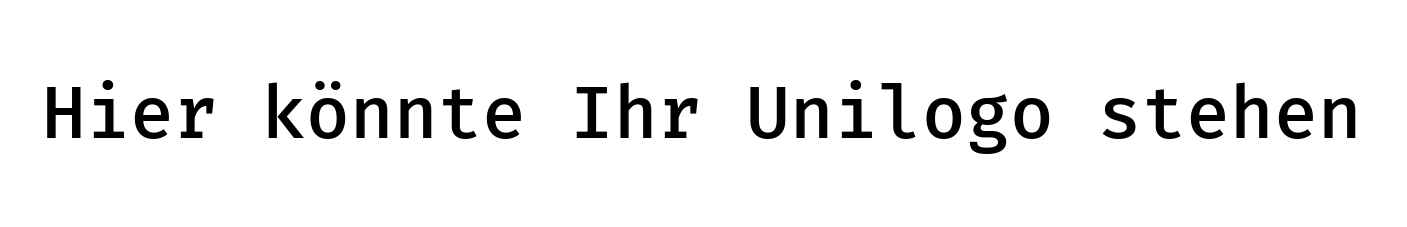
\includegraphics[width=8cm]{tud_logo_rgba}\\[\fill]
\noindent Gutachter:\\
\thefirstsupervisor\\
\thesecondsupervisor\\[2.5cm]
\begin{minipage}[b]{.55\textwidth}
Technische Universität Dortmund\\
Fakultät für Informatik\\
\thechair~(\thechairshort)\\
\url{\thechairurl}
\end{minipage}\hfill
%\begin{minipage}[b]{.45\textwidth}
%\raggedleft
%In Kooperation mit:\\
%Fakultätsname\\
%Lehrstuhl-/Institutsbezeichnung
%\end{minipage}
\end{titlepage}
%\newenvironment{cminted}
% {\RecustomVerbatimEnvironment{Verbatim}{BVerbatim}{}%
%  \def\FV@BProcessLine##1{%
%    \hbox{%
%      \hbox to\z@{\hss\theFancyVerbLine\kern\FV@NumberSep}%
%      \FancyVerbFormatLine{##1}%
%    }%
%  }%
%  \VerbatimEnvironment
%  \setbox\z@=\hbox\bgroup
%  \begin{minted}{coq}}
% {\end{minted}\egroup
%  \leavevmode\vbox{\hrule\kern2mm\box\z@\kern2mm\hrule}}
\makeatother
\shipout\null
\pagenumbering{roman}
%\pagecolor{white}
\restoregeometry
\tableofcontents
%\clearpage
\cleardoubleemptypage
\pagenumbering{arabic}
\chapter{Einleitung}

Aus der Softwareentwicklung wissen wir, dass Programmierer nicht unfehlbar sind. Ein wichtiges Werkzeug, das viele Sprachen bereitstellen, um Fehler zu vermeiden, ist die Typisierung. Variablen und Funktionen können so festen Typen zugewiesen werden, die einen Hinweis auf die Verwendung geben. Durch statische Analyse des Quelltextes kann dann überprüft werden, ob diese Hinweise beachtet werden. Betrachten wir hier die statisch typisierte Sprache \textsc{Java} mit dem folgenden Codefragment.
\begin{minted}{java}
public class Add {
  public static int add2(int i) {
      return i + 2;
  }
}
\end{minted}
Die Funktion \texttt{Add.add2} ist somit eine Funktion, die einen ganzzahligen Wert als Eingabe erwartet und einen ganzzahligen Wert als Rückgabe hat. Über das Typsystem von \textsc{Java} kann nun entschieden werden, dass \texttt{Add.add2(2)} einen gültigen, aber \texttt{Add.add2("{}Esel")} einen ungültigen Aufruf an \texttt{Add.add2} darstellt. Insbesondere wissen wir, dass \texttt{Add.add2(2)} selbst wieder eine ganze Zahl ist und infolgedessen \texttt{Add.add2(Add.add2(2))} ein gültiger Aufruf ist. Offensichtlich ist \texttt{Add.add2("{}Esel")} ein Programmierfehler. Für trivialen Fälle, wie der hier präsentierte, lässt sich dieser Fehler auch sehr schnell von Hand finden und würde in echten Softwareprojekten so natürlich nicht auftreten. Echte Softwareprojekte sind jedoch deutlich komplexer. Falls der String \texttt{"{}Esel"} nicht als Stringliteral, sondern über die Rückgabe einer anderen Funktion an \texttt{Add.add2} übergeben wird, lässt sich dies nicht mehr so einfach nachvollziehen. Der falsche Aufruf könnte hier beispielsweise durch eine Änderung der Schnittstelle oder durch die Verwechslung der entsprechenden Funktion auftreten. Je komplexer eine Software wird, desto höher ist die Wahrscheinlichkeit, dass solche Fehler auftreten. Typisierte Sprachen helfen diese Fehler bereits zur Compilezeit zu entdecken und verhindern so fehlerhaftes Verhalten in der Ausführung.

In dieser Arbeit werden wir uns mit dem theoretischen Konstrukt des \emph{einfach getypten Lambda-Kalküls} befassen. Dieser ist eine syntaktisch einfache Sprache zusammen mit einem einfachen Typsystem. Trotz dieser Einfachheit übertragen sich viele Ergebnisse, die im einfach getypten Lambda-Kalkül erforscht wurden, auf komplexere Typsysteme. Wir können somit den einfach getypten Lambda-Kalkül als Kern für diese komplexeren Typsysteme betrachten. Gerade wegen der Einfachheit können viele theoretische Aussagen einfacher getroffen und bewiesen werden. Der einfach getypte Lambda-Kalkül agiert nicht nur als Kern vieler Typsysteme, er entspricht sogar genau einem Fragment der Logik. Es gilt, dass Typen Aussagen entsprechen, und Terme, die zu diesen Typen passen, den Beweisen für diese Aussage entsprechen.\footnote{Dies werden wir im Rahmen dieser Arbeit auch betrachten.}

Wir werden in dieser Arbeit den Begriff des prinzipalen Typs betrachten. Der prinzipale Typ eines Terms ist der allgemeinste Typ eines Terms. Um eine Vorstellung zu bekommen, was ein allgemeinster Typ ist, betrachten wir erneut die Sprache \textsc{Java}, deren Typsystem Typvariablen über Generics unterstützt. Hierfür betrachten wir das folgende Codefragment.
\begin{minted}{java}
public class Id {
    public static int id(int i) { 
        return i;
    }
}
\end{minted}

Es ist klar, dass \texttt{Id.id} genau den Wert zurückgibt, den die Methode übergeben bekommt. Die hier angegebene Definition der Identität ist jedoch beschränkt auf \texttt{int}. Derselbe Methodenrumpf kann jedoch für die Identität beliebiger Typen verwendet werden. Mittels Generics können wir einen Typ für die Methode angeben, der nicht auf \texttt{int} beschränkt ist.

\begin{minted}{java}
public class Id_T {
  public static <T> T id(T i) { 
    return i;
  }
}
\end{minted}

Die Methode \texttt{Id\_T.id} typt hier den Term \texttt{return i;} mit seinem allgemeinsten Typen, \texttt{T $\to$ T}.

Eine wichtige Fragestellung im Umgang mit Typsystemen ist die der Inhabitation. Die Frage nach der Inhabitation ist die Frage, ob es zu einem gegebenen Typen einen Term gibt, der erfolgreich mit dem gegebenen Typen getypt werden kann. Diese Frage ist keineswegs trivial. Gehen wir davon aus, dass wir eine generische Typvariable \texttt{T} haben. Um \texttt{T} zu inhabitieren, müssten wir eine Funktion schreiben, die ohne Eingabe, jeden beliebigen Typen hat. Dies ist nicht ohne weiteres möglich\footnote{Tatsächlich kann in Java einfach \texttt{null} zurückgegeben werden, da \texttt{null} jeden Typ inhabitiert. In dieser theoretischen Behandlung betrachten wir jedoch diese und ähnliche Fälle nicht, in denen beliebige Typen inhabitiert werden können. Des Weiteren haben bestimmte Java- und Scalaversionen einen Fehler, der es erlaubt das Typsystem zu überlisten und beliebige Typen zu inhabitieren.\cite{unsound}}. 

Die Inhabitation ist in der Hinsicht interessant, da aus einem Algorithmus, der die Inhabitation entscheidet, auf einfache Art und Weise genau der Term extrahiert werden kann, der den Typ inhabitiert. Wenn über ein geeignetes Typsystem nun mittels Typen eine Spezifikation für Programme kodiert wird, lassen sich somit ganze Programme synthetisieren\cite{cls}. Des Weiteren lassen sich über den Zusammenhang zur Logik Aussagen über die Inhabitation von Typen, auf die Beweisbarkeit von logischen Aussagen übertragen.

Von besonderen Interesse ist hier auch die Frage der prinzipalen Inhabitation. Während die Frage der Inhabitation der Existenz eines Terms zu einem gegebenen Typen entspricht, entspricht die prinzipale Inhabitation der Existenz eins Terms, sodass der gegebene Typ der allgemeinste Typ des Terms ist. Übertragen auf die Synthese von Programmen entspricht dies einem Programm, dass genauestens einer Spezifikation entspricht; übertragen auf die Logik entspricht es einem Beweis, der nicht mehr beweist, als die gesuchte Aussage.

\cite{dudenhefner} zeigt, dass die Frage nach der prinzipalen Inhabitation weder deutlich schwieriger, noch deutlich einfacher als die der normalen Inhabitation zu beantworten ist. Beide Probleme sind \PSPACE-vollständig. Das Enthaltensein in \PSPACE{} folgt aus einem in \cite{dudenhefner} aufgestellten Algorithmus, der zum einen die prinzipale Inhabitation entscheidet und zum anderen die entsprechende Platzschranke einhält. Die \PSPACE-Schwierigkeit ist in \cite{dudenhefner} mit einer Reduktion von dem ebenfalls \PSPACE-vollständigen Problem der normalen Inhabitation, eingeschränkt auf eine bestimmte Art von Typen, bewiesen. Hierfür wird aus einem inhabitierten Typ $\tau$ ein prinzipal inhabitierter Typ $\tau^*$ erstellt, indem dieser mit Teiltypen von sich selber erweitert wird. Die genaue Konstruktion ist an dieser Stelle zunächst nebensächlich, relevant ist hier, dass der resultierende Typ $\tau^*$ stark von dem Ursprungstyp $\tau$ abhängt. Die Arbeit stellt des Weiteren die Vermutung auf, dass eine sehr ähnliche Konstruktion für Typen, die keiner Einschränkung unterliegen, möglich ist. 

Das Beantworten der Vermutung ist nicht Teil dieser Arbeit, es werden jedoch Grundlagen gelegt, diese computergestützt zu beweisen, sowie die in \cite{dudenhefner} geführten Beweise zu verifizieren. Insbesondere werden die dort genutzten Techniken der Teilformelfiltration sowie des Teilformelkalküls mittels des Beweishelfers \coq{} formalisiert. Hierfür wurden die wichtige Lemmata, die den Zusammenhang zwischen diesen Techniken und der prinzipalen Inhabitation zeigen, implementiert. \cite{dudenhefner} nennt beide Techniken die \emph{algorithmische Essenz} der prinzipalen Inhabitation. 

\section{Vorgehen}
Zunächst wird in \Cref{ch:stlc} der einfach getypte Lambda-Kalkül als theoretische Grundlage vorgestellt. Hierfür werden zunächst $\lambda$-Terme und einfache Typen unabhängig voneinander eingeführt. Anschließend werden diese in einem Kalkül miteinander verbunden. Zusätzlich werden grundlegende Lemmata aufgestellt und bewiesen, die helfen ein fundiertes Verständnis des einfach getypten Lambda-Kalküls zu erhalten, auf das in den nachfolgenden Kapiteln aufgebaut werden kann. Die Struktur des Kapitels, sowie ein Großteil der Definitionen folgt \cite{lecturesCH}.

Auf diesen Grundlagen aufbauend, wird in \Cref{ch:princ} die prinzipale Inhabitation sowie die in \cite{dudenhefner} vorgestellte Teilformelfiltration und der Teilformelkalkül präsentiert. Beide Techniken werden hierfür zunächst eingeführt und dann jeweils ein Bezug zur prinzipalen Inhabitation hergestellt. Hierfür werden die in \cite{dudenhefner} aufgestellten Lemmata sowie Beweise vorgestellt und die Ideen zu Letzteren verdeutlicht.

In \Cref{ch:coq} wird die im Rahmen dieser Arbeit angefertigte Formalisierung der Theorie beschrieben. Hierfür werden die in der Implementierung verwendeten Datentypen sowie Beweismechanismen vorgestellt um sowohl Lemma 14, als auch Lemma 25 aus \cite{dudenhefner} sowie der hierfür notwendigen Hilfslemmata zu verifizieren. Lemma 14 stellt einen Bezug zwischen der Teilformelfiltration und der prinzipalen Inhabitation her; Lemma 25 ist ein wichtiges Lemma, um einen Bezug zwischen dem Teilformelkalkül und der prinzipalen Inhabitation herzustellen\footnote{Diese entsprechen \Cref{lem:filtrprinc} und \Cref{lem:fz} in dieser Arbeit}. Die Beweise der weiteren Lemmata wurden aus Zeitgründen nicht implementiert, jedoch wurden diese zum Teil ohne Beweis formalisiert. Die Beweise und Formalisierungen werden mittels des Beweishelfers \coq{} in der Version 8.8.0 formuliert. Hierfür wird zudem die Bibliothek \textsc{Autosubst} verwendet, die speziell für die Handhabung von Substitutionen in Termen entwickelt wurde. In dem Kapitel werden nicht die Implementierungen der Beweise angegeben, sondern lediglich die Formalisierung der Lemmata aus \Cref{ch:princ}. Dies entspricht an dieser Stelle einer API-Dokumentation und soll sowohl helfen, die hier vorgestellte Implementierung nachzuvollziehen, als auch helfen, auf der Implementierung aufzubauen, um beispielsweise diese zu vervollständigen. Auch wird nicht jedes verwendete Lemma und jede verwendete Konstruktion explizit vorgestellt, da viele lediglich als Hilfestellung für die Implementierung der \emph{wichtigen} Lemmata fungieren. Von diesen Hilfskonstruktionen werden nur die Wichtigsten vorgestellt, sodass dies dem Verständnis der Beweisführung hilft.

Abschließend wird ein Fazit gezogen. Insbesondere wird evaluiert, inwieweit sich das Verifizieren in \coq{} und das schriftliche Beweisen unterscheiden. Zudem wird ein Ausblick gegeben, wie Prinzipalität in anderen Bereichen, als der Inhabitation betrachtet werden kann.
\renewcommand{\implies}{\Rightarrow}
\renewcommand{\impliedby}{\Leftarrow}
\newcommand{\V}{\ensuremath{\mathcal{V}}}
\newcommand{\At}{\ensuremath{\mathbb{A}}}
\newcommand{\T}{\ensuremath{\mathbb{T}}}
\newcommand{\tI}{\textbf{I}}
\newcommand{\tK}{\textbf{K}}
\newcommand{\tS}{\textbf{S}}
\newcommand{\tLambda}{\texorpdfstring{\ensuremath{\Lambda}}{Lambda}}
\newcommand{\tlambda}{\texorpdfstring{\ensuremath{\lambda}}{lambda}}
\newcommand{\talpha}{\texorpdfstring{\ensuremath{\alpha}}{alpha}}
\newcommand{\tbeta}{\texorpdfstring{\ensuremath{\beta}}{beta}}
\newcommand{\teta}{\texorpdfstring{\ensuremath{\eta}}{eta}}
\newcommand{\zB}{z.\,B. } 
\newcommand{\betared}{\ensuremath{\rightarrow_\beta}}
\newcommand{\msbetared}{\ensuremath{\twoheadrightarrow_\beta}}
\newcommand{\etared}{\ensuremath{\rightarrow_\eta}}
\newcommand{\msetared}{\ensuremath{\twoheadrightarrow_\eta}}
\newcommand{\etaexp}{\ensuremath{\rightarrow_\eta^{-1}}}
\newcommand{\msetaexp}{\ensuremath{\twoheadrightarrow_\eta^{-1}}}
\newcommand{\nat}{\ensuremath{\mathbb{N}}}
\newcommand{\IPCarr}{\ensuremath{\text{IPC}_\to}}
\newcommand{\STLC}{\ensuremath{\lambda_\to}}
\newcommand{\Long}{\text{Long}}
%\newcommand{\lam}{\ensuremath{\lambda}}


\chapter{Der einfach getypte Lambda-Kalkül}
\label{ch:stlc}

In diesem Kapitel werden die Grundlagen des einfach getypten Lambda-Kalküls ($\STLC$) vorgestellt, die wir in den späteren Kapiteln benötigen.
Der einfach getypte Lambda-Kalkül setzt sich aus den \tlambda-Termen und den einfachen Typen zusammen. Zunächst werden die Terme eingeführt, sowie eine Vorschrift, die es erlaubt Berechnungen über \tlambda-Terme durchzuführen. Des Weiteren werden Normalformen definiert, die insbesondere in den nachfolgenden Kapiteln wichtig werden.
 
Weiter werden die einfachen Typen eingeführt und diese mit den \tlambda-Termen kombiniert, um ein Typsystem zu erhalten und den Begriff der Inhabitation zu definieren und zu untersuchen.

Zuletzt werden wir eine alternative, aber äquivalente Definition der \tlambda-Terme kennenlernen, die es uns einfacher macht, computergestützt Aussagen über den einfach getypten Lambda-Kalkül aufzustellen und zu beweisen.
\section{\tlambda-Terme}
\tlambda-Terme sind eine Notation für funktionale Berechnungen. Wir werden zunächst \tlambda-Präterme betrachten und auf Basis derer die \tlambda-Terme definieren, die wir in diesem und dem nächsten Kapitel nutzen werden. Wir nutzen hier die Formalisierung aus \cite{lecturesCH}.
\begin{definition}{\tlambda-Präterm}{preterm}
    Sei \V{} eine abzählbar unendliche Menge an Variablensymbolen, dann sei die Menge $\Lambda^-$ der \emph{\tlambda-Präterme} die kleinste Menge mit den folgenden Eigenschaften.
\begin{align*}
    v\in\V&\implies v\in\Lambda^- & (\text{Variable})\\
    M, N \in\Lambda^-&\implies (M~N)\in\Lambda^- & (\text{Applikation})\\
    v\in\V\land M\in\Lambda^-&\implies (\lambda x.M)\in\Lambda^- & (\text{Abstraktion})
\end{align*}
\end{definition}
\begin{notation}
    Applikationen binden nach links und Abstraktionen nach rechts. Wir verzichten auf Klammerung, falls Zugehörigkeit über die Bindungsregeln eindeutig ist. Des Weiteren verzichten wir auf die äußerste Klammer eines Terms und fassen mehrere Abstraktionen zu einer zusammen.
    Anstelle der Terme \[(((M~N)~O)~P), (\lambda x.(\lambda y.x))\text{ und }((\lambda x.(P~Q))~R)\] schreiben wir
    \[M~N~O~P, \lambda x~y.x\text{ und }(\lambda x.P~Q)~R\].
\end{notation}
\begin{convention}
    Wir bezeichnen Terme üblicherweise mit Großbuchstaben aus der Mitte des Alphabets (\zB $M,N,P,Q$), und Variablen mit Kleinbuchstaben aus den letzten Buchstaben des Alphabets (\zB $x,y,z$).
\end{convention}
\begin{remark}
    Abstraktionen werden häufig anonyme Funktionen genannt. Anstelle eine Funktion direkt mit einem Namen zu definieren, wie beispielsweise $f(x) = x$, können wir mithilfe von \tlambda-Termen die Funktion unabhängig von ihrem Namen notieren. Selbstverständlich können wir den Term anschließend einen Namen zuweisen, $f = \lambda x.x$. Formal definieren wir dadurch nur die Berechnungsvorschrift einer Funktion, eine Funktion ist aber zusätzlich noch über ihren Definitions- und Wertebereich definiert. Wir werden diese Beobachtung in \Cref{sec:simpltypes} erneut betrachten.
\end{remark}
\begin{example}{}{}
\begin{itemize}
    \item Der Term $\lambda x.x$ entspricht der Funktion $f(x)=x$ und wird mit \tI{} abgekürzt.
    \item Der Term $\lambda x~y.x$ entspricht der Funktion $f(x, y)=x$ und wird mit \tK{} abgekürzt.
    \item Der Term $\lambda x~y~z.x~z~(y~z)$ entspricht der Funktion $f(x, y, z) = x(z)(y(z))$ und wird mit \tS{} abgekürzt.
    \item Der Term $x$ entspricht der Konstanten $x$. Hierbei ist zu bemerkten, dass wir Konstanten als nullstellige Funktionen auffassen können.
    \item Der Term $y~x$ entspricht $y(x)$ der Anwendung einer Funktion $y$ auf einen Term $x$.
\end{itemize}
\end{example}
\begin{remark}
    Die Terme \tS,\tK{} und \tI{} bilden die Grundlage des SKI-Combinator-Calculus.\cite{Schoenfinkel1924}    
\end{remark}

Wenn wir den Term $\lambda x.x$ und den Term $\lambda y.y$ betrachten, so entsprechen sie den Funktionen $f(x)=x$ und $f'(y)= y$. Es ist intuitiv klar, dass sich $f$ und $f'$ gleich verhalten. Sie nehmen eine Eingabe und geben diese unverändert zurück. Hierbei ist es unerheblich, ob die Eingabe $x$ oder $y$ genannt wird. Syntaktisch sind sie jedoch verschieden. Wenn wir rein die Konstruktion über die \tlambda-Präterme betrachten, folgt, dass $\lambda x.x \neq \lambda y.y$. 

Um diese intuitive Gleichheit zu formalisieren, führen wir zunächst Ersetzungen von Variablen in Termen ein. Darauf aufbauend werden zunächst wir eine Relation einführen, die nach unserer Intuition gleiche Terme in Relation setzt, also $\lambda x.x \sim \lambda y.y$, sowie einer Definition für \tlambda-Terme, in denen gilt $\lambda x.x = \lambda y.y$.
    
\subsection{Substitution}

Die Substitution ist die Grundlage des Berechnungsmodells im Lambda-Kalkül. Vereinfacht betrachtet ersetzen wir alle Variablen, die durch eine Abstraktion eingeführt werden durch einen Term, der durch die rechte Seite einer Applikation gegeben wird. Betrachten wir dazu zunächst, wie wir intuitiv einen \emph{Rechenschritt} mittels mathematischen Funktionen durchführen. Sei $f : \nat\to\nat$ eine Funktion, die mit $f(x) = x + 3$ definiert ist. Wollen wir nun $f(3)$ berechnen, ersetzen wir zunächst alle Vorkommen von $x$ durch $3$ und erhalten die nullstellige Funktion $3 + 3$, welche wir später weiter zu $6$ auswerten können.

Wir übertragen nun diese Intuition auf unsere \tlambda-Präterme. Sei $c_3$ ein \tlambda-Präterm, der der natürlichen Zahl $3$ entspricht und $A_+$ ein \tlambda-Präterm, der der (natürlichen) Addition entspricht\footnote{Die entsprechenden Terme existieren. Die Terme $c_n$ heißen Churchnumerale. Siehe hierfür \cite{lecturesCH}}, dann können wir den folgenden Term formulieren, der der Funktion $f$ entspricht \[\lambda x. A_+~x~c_3.\]


Wir können im \emph{inneren} \tlambda-Term alle $x$ durch $c_3$ ersetzen, um den Term $A_+~c_3~c_3$ zu erhalten. Wir schreiben $M[x/N]$ für den Term $M$, in dem die Variable $x$ durch den Term $N$ ersetzt wurde. Es gilt somit $(A_+~x~c_3)[x/c_3]=A_+~c_3~c_3$. Die Substitution verhält sich somit genau, wie unser intuitives Verständnis.

Aufpassen müssen wir bei geschachtelten Abstraktionen. Wir erinnern uns, dass in unserem intuitiven Verständnis gelten soll, dass $\lambda x.x\sim\lambda y.y$. Des Weiteren soll gelten, dass falls $M\sim N$ auch für alle $x$ und $P$ gelten soll, dass $M[x/P]\sim N[x/P]$. Betrachten wir die beiden Substitutionen $(\lambda x.x)[x/P]$ und $(\lambda y.y)[x/P]$. Wenn wir einfach alle Vorkommen von $x$ einer Variable durch $P$ ersetzen, erhalten wir die Terme $\lambda x.P$ und $\lambda y.y$. Klar ist, dass die Terme vor der Substitution intuitiv gleich sind, klar ist aber auch, dass $\lambda x.P$ und $\lambda y.y$ nicht zwangsweise gleich sind.
Um dies zu verhindern, müssen wir Abstraktionen besonders behandeln. Hierfür benötigen wir eine Definition von gebundenen und freien Variablen.
\begin{definition}{Freie Variable}{fv}
Sei $x\in\V$ und $M,N\in\Lambda^-$. Dann ist $FV:\Lambda^-\to\mathcal{P}(\V)$ mit 
\begin{align*}
FV(x) &= \{x\}\\
FV(M~N) &= FV(M)\cup FV(N)\\
FV(\lambda x.N) &= FV(M)\setminus \{x\}
\end{align*} eine Funktion, die einem Term seine freien Variablen zuweist.
Falls $y\in FV(M)$, nennen wir $y$ eine \emph{freie Variable} im Term $M$.
\end{definition}
Analog können wir die Menge der gebundenen Variablen definieren.
\begin{definition}{Gebundene Variable}{bv}
Sei $x\in\V$ und $M,N\in\Lambda^-$. Dann ist $BV:\Lambda^-\to\mathcal{P}(\V)$ mit
    \begin{align*}
    BV(x) &= \emptyset\\
    BV(M~N) &= BV(M)\cup BV(N)\\
    BV(\lambda x.N) &= BV(N)\cup\{x\}
    \end{align*} eine Funktion, die einem Term seine gebundenen Variablen zuweise.
    Falls $y\in BV(M)$, nennen wir $y$ eine \emph{gebundene Variable} im Term $M$.
\end{definition}
\begin{remark}
    Eine Variable kann gleichzeitig als freie und als gebundene Variable in einem Term vorkommen.
    \[x\in BV(x~\lambda x.x) \text{ und } x\in FV(x~\lambda x.x)\]
\end{remark}

\begin{definition}{Geschlossener Term}{closed}
    Ein Term $M$ ist geschlossen, wenn $FV(M)=\emptyset$.
\end{definition}

Wir könnten nun eine Substitution angeben, die genau die freien Variablen eines Term ersetzt. In unserem obigen Beispiel gelte dann folgendes.
\[(\lambda x.x)[x/N] = \lambda x.x \sim \lambda y.y = (\lambda y.y)[x/N]\]

Wir müssen zusätzlich noch darauf achten, dass eine Substitution keine bereits vorhandenen gebundenen Variablen als freie Variablen einführt. Betrachten wir dazu die Substitution \((\lambda x.y)[y/x] \). Wenn gelten soll, dass $\lambda x.y \sim \lambda z.y$, da auch die Funktionen $f(x) = y$ und $f'(z) = y$ identisch sind, gilt ebenfalls $(\lambda x.y)[y/x] \sim (\lambda z.y)[y/x]$, also $\lambda x.x\sim\lambda z.y$. 
Es ist auch klar, dass die Gleichheit $\lambda x.x = \lambda z.x$ nicht mit unserem intuitiven Verständnis übereinstimmt. Um zu verhindern, dass eine gebundende Variable als freie Variable in dem einzusetzenden Term vorkommt, können wir die gebundene Variable zuvor durch eine unbenutzte Variable ersetzen und damit eine Substitutionsvorschrift definieren, die unsere intuitive Gleichheit von Termen respektiert.

\begin{definition}{Frische Variable}{fresh}
    Eine Variable $x$ ist genau dann \emph{frisch} in einem Term $M$, wenn sie weder als freie, noch als gebundene Variable vorkommt.
\end{definition}
\begin{proposition}{}{fresh}
    Zu jedem Term $M$ gibt es unendlich viele Variablen, die frisch sind.
    \Proof Jeder Term $M$ ist endlich, damit ist die Menge der vorkommenden Variablen endlich. Eine Variablenmenge \V{} ist abzählbar unendlich.    
\end{proposition}
\begin{definition}{Substitution}{subst}
    Sei $M, P\in\Lambda^-$, $z\in\V$ frisch in $M$ und $P$, $x,y\in\V$ mit $x\neq y$. Wir definieren die \emph{Substitution} $M[x/P]$ durch Fallunterscheidung über $M$.
    \begin{align*}
    x[x/P] &= P\\
    y[x/P] &= y\\
    (M~N)[x/P] &= M[x/P]~N[x/P]\\
    (\lambda y.N)[y/P] &= \lambda y.N\\
    (\lambda x.N)[y/P] &=\begin{cases}
    \lambda z.N[x/z][y/P]& \text{Falls x}\in FV(P)\cap FV(N)\\
    \lambda x.N[y/P]& \text{sonst}
    \end{cases}
    \end{align*}
\end{definition}
\begin{remark}
    \begin{itemize}
        \item In der Literatur gibt es für die Substitution verschiedene Notationen. Wir folgen hier \cite{Troelstra1996}, sodass wir eine Substitution $[a/b]$ als das Ersetzen von $a$ durch $b$ lesen. Es gibt auch die Lesart, sodass wir $b$ durch $a$ ersetzen.\cite{curry}
    \item Es gibt aufgrund \Cref{prop:fresh} immer eine frische Variable $z$, die wir wählen können.
        \item Wir nennen eine Substitution durch eine Variable auch eine Umbenennung.
        \end{itemize}    
\end{remark}

Das folgende Lemma beweist die Intuition, dass falls eine Variable nicht in der Definition einer Funktion (frei) vorkommt, eine Ersetzung den Term nicht beeinflusst.

\begin{lemma}{}{freesubst}
    Für alle $x\in\V$, $M,N\in\Lambda$ gilt, falls $x\notin FV(M)$, dann gilt $M[x/P] = M$
    \Proof
    Durch Induktion über M.
    \begin{description}
        \item[Fall (IA) $M = y$:] 
        \[x\notin FV(y)\implies x \neq y \implies y[x/P] = y\]
        \item[Fall $M = P~Q$:]  
        \begin{align*}
        x\notin FV(P~Q)&\implies x \notin FV(P) \land x \notin FV(Q)\\
        &\overset{IH}{\implies} P[x/N] = P \land Q[x/N] = Q \\
        &\implies (P~Q)[x/N)=P~Q
        \end{align*}      
        \item[Fall $M = \lambda y.P$ und $x \neq y$:] 
        \begin{align*}
        &x\notin FV(\lambda y.P)\land x\neq y \\
        & \implies x\notin FV(P) \overset{IH}{\implies}P[x/N]=P\\
        &\implies \lambda y.P[x/N] = \lambda y.P \\
        &\implies (\lambda y.P)[y/N] = \lambda y.P
               \end{align*}        
        \item[Fall $M = \lambda x.N$:] 
        \[\lambda x.N[x/P]=\lambda x.N\]
    \end{description}
\end{lemma}

Wir können nun formulieren, dass zwei Terme in einer Art und Weise gleich sind, wenn sie sich nur in den Namen ihrer gebundenen Variablen unterscheiden.

\begin{definition}{\talpha-Äquivalenz}{alphaequiv}
    Seien $x,y\in\V$ Variablen, $N, N', M, M'\in\Lambda^-$ \tlambda-Präterme. Wir definieren die \talpha-Äquivalenz $\equiv_\alpha$ als kleinste transitive, reflexive und symmetrische Relation (Äquivalenzrelation) mit den folgenden Eigenschaften.
    \begin{align*}        
     \lambda x.M &\equiv_\alpha \lambda y.M[x/y]\\  
    M\equiv_\alpha M' \implies \lambda x.M &\equiv_\alpha \lambda x.M'\\
    M\equiv_\alpha M' \implies N~M&\equiv_\alpha N~M'\\
    N\equiv_\alpha N' \implies N~M&\equiv_\alpha N'~M.
    \end{align*}
\end{definition}

Mit der \talpha-Äquivalenz haben wir nun eine Relation für $\sim$, unter der die von uns als intuitiv gleich angesehenen Terme äquivalent sind. Dies können wir nun zu einem Begriff erweitern, der es uns erlaubt, diese äquivalenten Terme als gleich anzusehen.

\begin{definition}{\tlambda-Terme}{term}
    Sei $[M]_\alpha$ die Äquivalenzklasse des \tlambda-Präterms $M$ unter der Relation $\equiv_\alpha$, dann ist die Menge der \tlambda-Terme \tLambda{} definiert als
    \[\Lambda=\{[M]_\alpha\mid M\in\Lambda^-\}\]
\end{definition}
\begin{notation}
Wir werden implizit die Äquivalenzklasse weglassen, sodass wir anstelle $[\lambda x.x]_\alpha\in\Lambda$,
direkt $\lambda x.x\in\Lambda$ schreiben, es gilt somit $\lambda x.x = \lambda y.y$.
\end{notation}
\begin{remark}
    In der Literatur werden \tlambda-Terme häufig wie unsere \tlambda-Präterme definiert und anstelle der Gleichheit zwischen Termen wird nur eine Äquivalenz unter der \talpha-Äquivalenz angegeben. Unsere explizite Unterscheidung zwischen $\Lambda$ und $\Lambda^-$ erlaubt es uns echte Gleichheiten zwischen \tlambda-Termen für unser intuitives Verständnis von Gleichheit zu verwenden. Siehe hierzu auch \cite{lecturesCH}.
\end{remark}

Das folgende Lemma erlaubt es uns, die Reihenfolge von Substitutionen zu ändern.

\begin{lemma}{Substitutionslemma}{subst}
    Seien $M, N, P\in\Lambda$ \tlambda-Terme, $x, y\in\V$ Variablen mit $x\neq y$ und $x\notin FV(P)$, dann gelte :
    \[M[x/N][y/P]=M[y/P][x/N[y/P]]\]
    \Proof
    Siehe \cite{lecturesCH}.
\end{lemma}


\subsection{\tbeta-Reduktion}
Wir können mittels \tlambda-Termen nun Funktionen und Funktionsanwendungen notieren, haben aber noch keine Vorschrift, nach der wir Berechnungen ausführen können. Genauer fehlt uns eine Vorschrift, die eine Applikation einer Abstraktion und einen anderen Term zusammenführt. Betrachten wir erneut mathematische Funktionen. Wenn wir eine einstellige Funktion $f(x) = M$ haben und zu einen zu $f$ \emph{passenden}\footnote{Wir werden in \Cref{sec:simpltypes} uns damit befassen, was es bedeutet, dass ein Wert \emph{passend} für einen Term ist.} Wert $N$, können wir die Anwendung von $f$ auf $N$, also $f(N)$ berechnen, indem wir in $M$ alle $x$ durch $N$ substituieren. In den \tlambda-Termen entspräche dies einem Übergang von $(\lambda x.M)~N$ zu $M[x/N]$. 

\begin{definition}{Redex}{redex}
    Sei $x\in\V$ eine Variable und $M, N\in\Lambda$ zwei \tlambda-Terme. Wir nennen einen Term in der Form $(\lambda x.M)~N$ einen Redex.
\end{definition}

\begin{definition}{\tbeta-Reduktion}{betared}
    Sei $x\in\V$, $M, N, M', N'\in\Lambda$, dann definieren wir die \tbeta-Reduktion $\betared$ als kleinste Relation mit den folgenden Eigenschaften.
    \begin{align*}
    (\lambda x.M)~N&\betared M[x/N]\\
    M\betared M' \implies \lambda x.M&\betared \lambda x.M'\\
    M\betared M' \implies  M N&\betared M'~N\\
    N\betared N' \implies  M N&\betared M~N'    
    \end{align*}
\end{definition}
\begin{remark}
    Die \tbeta-Reduktion ersetzt genau einen Redex in einem Term. Der transitiv-reflexive Abschluss der \tbeta-Reduktion \msbetared, die sogenannte \emph{multi-step \tbeta-Reduktion}, ersetzt beliebig viele Redexe -- auch keinen -- in einem Term.
\end{remark}
Über die \tbeta-Reduktion können wir nun Rechnungen durchführen. Es ist sogar so, dass durch diese Relation der Lambda-Kalkül \emph{Turingvollständig} ist \cite{churchturing}\footnote{Der Lambda-Kalkül ist sogar älter als das Konzept der Turingmaschine. Vor der Einführung der Turingmaschine wurde Berechenbarkeit als \tlambda-Definierbarkeit über den Lambda-Kalkül definiert\cite{churchturing}.}. Wir werden in \Cref{ssec:nf} das Konzept \emph{Reduktion als Berechnung} aufgreifen und beschreiben, wann eine solche Berechnung terminiert.
\begin{example}{}{}
    \begin{itemize}
        \item $(\lambda x~y.x)~z\betared (\lambda y.x)[x/z] = \lambda y.x[x/z] = \lambda y.z$
        \item $(\lambda x.x~y)~(\lambda x.x)\betared (x~y)[x/\lambda x.x]= (\lambda x.x)~y \betared x[x/y]=y$
    \end{itemize}
\end{example}
\subsection{\teta-Reduktion}
Zwei weitere Relation, die wir einführen, sind die \teta-Reduktion und die \teta-Expansion. Die Grundidee hierbei ist es, \emph{unnötige} Abstraktionen zu vermeiden, bzw. explizit einen Term in eine weitere Abstraktion einzubetten. Wenn wir eine Abstraktion haben, die ihre abstrahierte Variable nur an ihren inneren Term weitergibt, können wir die Abstraktion auch weglassen, ohne das Verhalten des Terms zu ändern. Andersherum können wir jeden Term auch in zusätzliche Abstraktionen einbetten.
\begin{example}{}{eta}
    Betrachten wir den Term $(\lambda x.N~x)~M$ mit $x\notin FV(N)$. Nach den Regeln der \tbeta-Reduktion gilt $(\lambda x.N~x)~M\betared (N~x)[x/M] = N M$, jedoch gilt nicht $\lambda x.N x \betared N$. 
\end{example}
Es liegt nun nahe, dass $\lambda x.N x$ und $N$ aus \Cref{ex:eta} in einer geeigneten Relation zueinander stehen.
\begin{definition}{\teta-Reduktion}{etared}
    Sei $x,z\in\V$ eine Variable und $M,N\in\Lambda$ ein \tlambda-Term. Sei weiter $z\notin FV(N)$, dann definieren wir die \emph{\teta-Reduktion} $\etared$ als kleinste Relation mit den folgenden Eigenschaften.
    \begin{align*}
    \lambda z.N~z &\etared N\\
    M\etared M' \implies \lambda x.M&\etared \lambda x.M'\\
    M\etared M' \implies  M N&\etared M'~N\\
    N\etared N' \implies  M N&\etared M~N'        
    \end{align*}
\end{definition}
Analog dazu lässt sich die \teta-Expansion definieren.
\begin{definition}{\teta-Expansion}{etaexp}
    Sei $x,z\in\V$ eine Variable und $M,N\in\Lambda$ ein \tlambda-Term. Sei weiter $z\notin FV(N)$, dann definieren wir die \emph{\teta-Expansion} $\etaexp$ als kleinste Relation mit den folgenden Eigenschaften.
    \begin{align*}
    N &\etaexp \lambda z.N~z\\
    M\etaexp M' \implies \lambda x.M&\etaexp \lambda x.M'\\
    M\etaexp M' \implies  M N&\etaexp M'~N\\
    N\etaexp N' \implies  M N&\etaexp M~N'        
    \end{align*}
\end{definition}
\begin{remark}
    Analog zur \tbeta-Reduktion sind $\msetared$ und $\msetaexp$ die transitiv-reflexive Abschlüsse der \teta-Reduktion und \teta-Expansion.
\end{remark}
\subsection{Normalformen}
\label{ssec:nf}
Aufbauend auf den eingeführten Reduktionsregeln können wir nun Normalformen einführen, also Formen, in den die jeweilige Reduktion nicht mehr anwendbar ist. Wenn ein Reduktionsschritt ein Berechnungsschritt ist, ist eine Normalform das Ergebnis der Berechnung.

\begin{definition}{\tbeta-Normalform}{betanf}
    Ein Term $M$, zu dem es keinen Term $N$ gibt, sodass $M\betared N$, ist in \tbeta-Normalform.
\end{definition}

\begin{remark}
    Es gibt \tlambda-Terme, die keine \tbeta-Normalform haben, also deren Berechnung nicht terminiert. Dies ist insbesondere ein wichtiges Kriterium für die Turingvollständigkeit des Lambda-Kalküls. Betrachten wir den Term $\Omega = (\lambda x. x~x)~(\lambda x.x~x)$. Der Term enthält einen Redex, somit lässt er sich \tbeta-reduzieren. Eine Reduktion führt jedoch direkt wieder zu dem Term $\Omega$
    \begin{align*}
        \Omega&=(\lambda x.x~x)~(\lambda x.x~x)\betared (x~x)[x/\lambda x.x~x] \\&= x[x/\lambda x.x~x]~x[x/\lambda x.x~x]=(\lambda x.x~x)~(\lambda x.x~x)\\&=\Omega
    \end{align*}    
\end{remark}
\begin{remark}
Terme, die mehrere Redexe haben, stehen mit mehreren verschiedenen \tlambda-Termen gemäß der \tbeta-Reduktion in Relation. Die \tbeta-Reduktion ist somit nicht eindeutig.
\end{remark}

Auch zu der \teta-Reduktion können wir einen Normalformbegriff definieren. 

\begin{definition}{\teta-Normalform}{etanf}
    Ein Term $M$, zu dem es keinen Term $N$ gibt, sodass $M\etared N$ ist in \teta-Normalform.
\end{definition}

Wir werden in \Cref{longnf} eine Art Normalformbegriff für die \teta-Expansion kennenlernen.

\begin{figure}
    \center
    \begin{tikzpicture}[node distance=2cm]
    \node (M) at (0,0) {$M$};
    \node (P) [below left of = M] {$P$};    
    \node (Q) [below right of = M] {$Q$};
    \node (Z) [below right of = P] {$Z$};
    \path[draw, ->>] (M) -> (P);
    \path[draw, ->>] (M) -> (Q);
    \path[draw, dashed , ->>] (Q) -> (Z);        
    \path[draw, dashed , ->>] (P) -> (Z);        
    \end{tikzpicture}
    \caption{Diamanteigeschaft}
    \label{fig:diamond}    
\end{figure}

Im Folgenden werden Wir feststellen, dass es für das Ergebnis der Berechnung eines \tlambda-Terms unerheblich ist, in welcher Reihenfolge wir Redexe auflösen. Zunächst führen wir eine Eigenschaft ein, die besagt, dass die Wahl des Abzuleitenden Subterms in einer Reduktion in der Hinsicht nicht relevant ist, dass wir immer zu einem gemeinsamen Ergebnisterm gelangen können.

\begin{definition}{Diamanteigenschaft}{diamond}
    Seien $M,P,Q\in\Lambda$ \tlambda-Terme, dann sagen wir, dass eine transitiv-reflexive Relation $\twoheadrightarrow$ die Diamanteigenschaft erfüllt oder konfluent ist, wenn
    \[M\twoheadrightarrow P \land M\twoheadrightarrow Q\implies \exists Z\in\Lambda. P\twoheadrightarrow Z \land Q\twoheadrightarrow Z. \]
    Siehe hierfür auch \Cref{fig:diamond}.
\end{definition}
\begin{proposition}{Church-Rosser}{diamond}
    $\msbetared$ und $\msetared$ erfüllen die Diamanteigenschaft.
    \Proof
%    Grundsätzlich gilt, wenn $M$ in Normalform ist, muss $M = P = Q$ gelten. Damit existiert ein $Z$ mit $Z = P = Q = M$.
%    \begin{enumerate}
%        \item Induktion über $M$.
%        \begin{description}
%            \item[Fall $M=x$:] $x$ ist in Normalform.
%            \item[Fall $M=\lambda x.N$:] $P$ und $Q$ müssen in der Form $\lambda x.P'$ und $\lambda x.Q'$ mit $N\msbetared P'$ und $N\msbetared Q'$ sein. Nach Induktionshypothese gibt es ein $Z'$, sodass $P'\msbetared Z'$ und $Q'\msbetared Z'$. Somit gilt auch $P\msbetared \lambda x.Z'$ und $Q\msbetared \lambda x.Z'.$
%            \item[Fall $M=S~T$:] Hier unterscheiden wir 2 Fälle. $M$ selbst ist ein Redex oder ein Subterm von $S$ bzw. $T$ ist ein Redex, aber $M$ selbst nicht.
%            \begin{description}
%                \item[$M$ ist ein Redex] 
%            \end{description}
%        \end{description}
%        Fall M = x:
%
%        Fall $M = \lambda x.N$:
%          
%        Fall M = P'~Q':
%          
%    \end{enumerate}
Siehe \cite{lecturesCH}.
\end{proposition}     

Dies können wir nun erweitern, um festzustellen, dass eine Normalform -- also ein Ergebnis einer Berechnung -- nicht davon abhängt, in welcher Reihenfolge Redexe ausgewertet werden.

\begin{lemma}{Eindeutigkeit von Normalformen}{nfuniq}
    Seien $N_1$ und $N_2$ zwei Normalformen eines Terms $M$ zu einer Relation, dessen transitiv-reflexiver Abschluss die Diamanteigenschaft erfüllt, dann ist $N_1 = N_2$.
    \Proof
    Folgt direkt aus der Diamanteigenschaft. Ein Term in Normalform steht nur mit sich selbst in Relation, also $N_1 \twoheadrightarrow Z \implies Z = N_1$ und $N_2 \twoheadrightarrow Z \implies N_2 = Z$. Daher gilt $Z = N_1 = N_2$.
\end{lemma}
\section{Einfache Typen}
\label{sec:simpltypes}
Betrachten wir erneut Funktionen. Funktionen sind üblicherweise nicht nur durch ihren Funktionsrumpf definiert, sondern auch durch ihren Definitionsbereich (Domain) und Wertebereich (Codomain). Eine vollständige Definition für eine Funktion wäre die folgende:
\begin{align*}
f&:\nat\to\nat\\
f(x) &= x + 3
\end{align*}
Wir können hier $\nat\to\nat$ als Typ für die Funktion $f$ sehen. Die Menge der natürlichen Zahlen ist dann ein Typ für die Eingabe $x$ sowie für alle Ergebnisse von $f$. Betrachten wir den Aufbau des Typen $\nat\to\nat$. Dieser besteht aus zwei Komponenten, ein zweistelliger Operator $\to$ und die atomaren Typen $\nat$. 

Wir können ebenfalls der Identitätsfunktion $id(x) = x$ einen Typen geben. Die Domain und Codomain von $id$ ist durch die Definition nicht gegeben, es ist jedoch klar, dass die Codomain zumindest die Domain enthalten muss. Sei die Domain vom $id$ eine beliebige Menge $A$, so ist die Codomain mindestens eine Menge $B$ mit $A\subseteq B$. Insbesondere gilt $id : A \to A$. Dieses Prinzip können wir auf \tlambda-Terme erweitern. Es gibt es viele Typsysteme, die den Lambda-Kalkül typen, wir betrachten hier die einfachen Typen.
\begin{definition}{Einfache Typen}{simpletypes}
    Sei \At{} eine abzählbar unendliche Menge an Typatomen, dann ist die Menge \T{} der einfachen Typen definiert als kleinste Menge mit den folgenden Eigenschaften:
    \begin{align*}
    a\in\At&\implies a\in\T\\
    \alpha, \beta\in \T&\implies \alpha\to\beta\in\T
    \end{align*}
 \end{definition}
\begin{convention}
Wir bezeichnen Typen mit kleinen griechischen Buchstaben (\zB $\alpha,\beta$ aber auch $\sigma, \tau, \rho$), Typatome mit kleinen Buchstaben aus den ersten Buchstaben des Alphabets (\zB $a,b,c$)
\end{convention}
\begin{definition}{Teiltyp}{subformula}
    Sei $\rho\in\T$ ein einfacher Typ, dann ist die Menge $\text{codom}(P_\rho)$ seiner Teiltypen folgendermaßen induktiv definiert.
    \begin{align*}
        \text{codom}(P_b) &= b &\text{für }b\in\At\\
        \text{codom}(P_{\sigma\to\tau}) &= 
        \begin{aligned}[t]
         &\{\sigma\to\tau\}~\cup\\
         &\text{codom}(\sigma)~\cup\\
         &\text{codom}(\tau)
        \end{aligned}
    \end{align*}
    
    Falls $\rho'\in\text{codom}(\rho)$, aber $\rho \neq \rho'$, dann nennen wir $\rho'$ einen echten Teiltypen von $\rho$.
\end{definition}
\begin{remark}
    \begin{itemize}
        \item Die Benennung der Menge der Teiltypen deutet bereits an, dass $P_\rho$ eine Funktion darstellt. Dies ist der Fall und sie wird in \Cref{def:path} definiert.
        \item In der Literatur wird anstelle von Teiltypen auch von Subformelen gesprochen. Dies hängt mit dem \emph{Curry-Howard-Isomorphismus} zusammen, der besagt, dass Typen Formeln darstellen. Wir werden dies in \Cref{sec:IPC} betrachten.
    \end{itemize}
\end{remark}
Analog zu den Variablen in \tlambda-Termen können wir für Typatome in einfachen Typen eine Definition für unbenutzte, frische Variablen aufstellen.
\begin{definition}{Frisches Typatom}{freshat}
    Wir nennen ein Atom $a$ \emph{frisch} in einem Typen $\rho$, wenn es nicht als Teiltyp von $\rho$ auftaucht.
\end{definition}
\section{Typisierung}
Wir benötigen nun einen Kalkül, mit dem wir Terme und Typen in Relation setzen können. Es ist auffällig, dass $\lambda x.M$ eine (mindestens einstellige) Funktion darstellt und $\alpha\to\beta$ ein Funktionstyp ist. Interpretieren wir $\alpha$ als Domain und $\beta$ als Codomain der Funktion, müssen alle Terme $N$, auf die die Funktion angewendet wird, den Typen $\alpha$ haben und der Term $M[x/N]$ den Typen $\beta$.
Da $N$ den Typen $\alpha$ hat, muss $x$ in $M$ auch den Typen $\alpha$ haben. Wir müssen uns also merken, dass in $M$ die Variable $x$ mit $\alpha$ getypt wird. Dazu müssen wir uns einen Typkontext merken, der Variablen Typen zuweist. Wir führen hierfür eine Relation $\Gamma\vdash M:\rho$ ein, die aussagt, dass zu einem Typkontext $\Gamma$ der Term $M$ mit dem Typen $\rho$ getypt werden kann.

\begin{definition}{Typkontext}{context}
    Ein Typkontext $\Gamma$ ist eine Relation mit $\Gamma\subseteq \V\times\T$, bei der alle Elemente aus $\V$ maximal einmal in der Domain der Relation vorkommen dürfen.
\end{definition}
\begin{notation}
    Wir schreiben Elemente $(x,\rho)$ aus $\Gamma$ als $x : \rho$. Des Weiteren schreiben wir $\Gamma, x:\rho$ anstelle von $\Gamma\cup(x,\rho)$. Hierbei ist zu beachten, dass die Bedingung an Typkontexte nicht verletzt wird, da durch das Hinzufügen eine Variable mit mehreren Typen getypt werden könnte.
\end{notation}

\begin{definition}{Typisierung}{typing}
    Seien $\Gamma\subseteq\V\times\T$ ein Typkontext, $\sigma,\tau,\rho\in\T$ einfache Typen, $M, N\in\Lambda$ \tlambda-Terme und $x\in\V$ eine Variable. Wir definieren die Typisierung $\_ \vdash \_ : \_$ anhand folgender Inferenzregeln.
  \[\infer[\var]{\Gamma,x:\rho\vdash x : \rho}{}\]
  \[\infer[\abs]{\Gamma\vdash\lambda x.M : \sigma\to\tau}{\Gamma, x:\sigma\vdash M:\tau}\]
  \[\infer[\app]{\Gamma\vdash M~N :\tau}{\Gamma\vdash M : \sigma\to\tau&\Gamma\vdash N : \sigma}\]
  
  Wir bezeichnen einen Baum $\mathcal{D}$ mit Wurzel $\Gamma\vdash M : \rho$, der sich durch die Anwendung der obigen Inferenzregeln ergibt, als Typableitung. Wenn $\mathcal{D}$ die Typableitung zu der Typisierung $\Gamma\vdash M : \rho$ ist, schreiben wir auch $\mathcal{D}\judges\Gamma\vdash M:\rho$.
  
\end{definition}
\begin{notation}
    Anstelle von $\emptyset\vdash M : \rho$ schreiben wir auch $\vdash M:\rho$.
\end{notation}

Jede Art, einen \tlambda-Term $M$ zu konstruieren, korrespondiert zu genau einer Typisierungsregel. Betrachten wir den äußersten Konstruktor von $M$, lässt sich ablesen, welche Regel genutzt wurde, um $M$ zu typen. Dies wird im folgenden Generierungslemma formalisiert.

\begin{lemma}{Generierungslemma}{simplgen}
    Sei $\Gamma\subseteq\V\times\T$ ein Typkontext, $M\in\Lambda$ ein \tlambda-Term und $\rho\in\T$ ein einfacher Typ. Gelte weiter $\Gamma\vdash M:\rho$. Dann gilt
    \begin{itemize}
        \item falls $M = x$, $x : \rho\in\Gamma$
        \item falls $M = \lambda x.N$, $\rho = \sigma\to\tau$ sodass $\Gamma, x:\sigma\vdash N:\tau$
        \item falls $M = P~Q$, es existiert ein $\sigma$, sodass $\Gamma\vdash M:\sigma\to\rho$ und $\Gamma\vdash N:\sigma$
    \end{itemize}
    \Proof
    In jedem Beweisschritt ist es eindeutig, welche Regel gewählt wird. 
\end{lemma}

\begin{definition}{Typbar}{typable}
Terme, zu denen es ein $\Gamma$ und ein $\rho$ gibt, sodass $\Gamma\vdash M : \rho$, nennen wir typbar.
\end{definition}

\begin{example}{}{typable}
    \begin{enumerate}
        \item Der Term $\tI$ ist typbar mit $\vdash\tI:\alpha\to\alpha$
        \item Der Term $x~x$ ist nicht typbar. 
    \end{enumerate}
\Proof
\begin{enumerate}
      \item \[
    \infer[(abs)]{\vdash \lambda x.x:\alpha\to\alpha}{\infer[(var)]{x:\alpha\vdash x : \alpha}{}}
    \]
    \item Es ist klar, dass $x~x$ in einem Kontext, der nicht $x$ enthält, nicht typbar ist. Nehmen wir an, dass es eine Typisierung $\Gamma,x:\alpha\vdash x~x:\rho$ gibt. Laut \Cref{lem:simplgen} gibt es ein $\sigma$, sodass $\Gamma, x:\alpha\vdash x:\sigma\to\rho$ und $\Gamma, x:\alpha\vdash x:\sigma$.
    
    Weiter folgt nach \Cref{lem:simplgen}, dass $\alpha=\sigma=\sigma\to\rho$ gelten muss. Die Gleichung $\sigma = \sigma\to\rho$ kann für endliche Typen nicht erfüllt werden, und \Cref{def:simpletypes} erlaubt nur endliche Typen.	    
    \end{enumerate}
\end{example}

\begin{lemma}{Subtypbar}{subtypable}
    Sei $M\in\Lambda$ ein \tlambda-Term, der typbar ist. Dann ist jeder Subterm von $M$ ebenfalls typbar.
    \Proof
    Folgt direkt aus \Cref{lem:simplgen}.
\end{lemma}

\begin{definition}{Inhabitanten}{inhab}
    Falls $\vdash M:\rho$, nennen wir $M$ einen Inhabitanten von $\rho$ und $\rho$ inhabitiert.
\end{definition}

\begin{lemma}{Subject-Reduction}{subjred}
    Falls $\Gamma\vdash M:\rho$ und $M \msbetared N$, dann $\Gamma\vdash N:\rho$.
    \Proof
    Siehe \cite{lecturesCH}.    
\end{lemma}
\begin{remark}
    Die umgekehrte Richtung gilt nicht. Betrachten wir die Terme $\tI$ und $\tK~\tI~\Omega$. Es gilt $\tK~\tI~\Omega\betared\tI$ und $\vdash \tI:\alpha\to\alpha$, es gilt jedoch nicht, dass $\vdash\tK~\tI~\Omega:\alpha\to\alpha$. Es ist sogar so, dass $\tK~\tI~\Omega$ nicht typbar ist, da $x~x$ ein Subterm von $\Omega$ ist und $x~x$ nicht typbar ist. Siehe \Cref{lem:subtypable} und \Cref{ex:typable}.
\end{remark}

\begin{definition}{Typsubstitution}{typesubst}
Eine Funktion $Su : \At\to\T$ nennen wir Typsubstitution. 
Wir können eine Substitution $Su$ zu einer Funktion $Su^*$ homomorph auf Typen fortsetzen.
\begin{align*}
Su^* &: \T\to\T\\
Su^*(\rho) &=\begin{cases}
Su(\rho) & \text{falls } \rho\in\At\\
Su^*(\sigma)\to Su^*(\tau) & \text{falls } \rho = \sigma\to\tau
\end{cases}
\end{align*}
Weiter können wir eine auf Typen fortgesetzte Substitution $Su^*$ auf Typkontexte zu einer Funktion $Su^{**}$ fortsetzen.
\begin{align*}
Su^{**} & : (\T\times\V)\to(\T\times\V)\\
Su^{**}(\Gamma) & = \{x : Su^*(\rho)\mid x : \rho\in\Gamma\}
\end{align*}
\end{definition}
\begin{notation}
    Da $Su^{**}, Su^*$ und $Su$ in ihren Domain disjunkt, bzw. im Fall von $Su$ und $Su^*$ über einander definiert sind, schreiben wir für alle nur $Su$.
\end{notation}

Wir können noch einen Zusammenhang zwischen geschlossenen Termen und Termen, die sich in einem leeren Kontext typen lassen feststellen. 

\begin{lemma}{}{closed}
    Sei $M$ ein \tlambda-Term und $\rho$ ein einfacher Typ. Falls $\vdash M : \rho$, dann ist $M$ ein geschlossener Term.
    \Proof
    Wir zeigen die allgemeinere Aussage, dass ein Typkontext mindestens die freien Variablen in $M$ typen muss, durch Induktion über $M$. Durch \Cref{lem:simplgen} können wir direkt auf die Regel schließen, die für jeden Term genutzt wurde.
    \begin{description}
        \item[Induktionsanfang, $\Gamma\vdash x : \rho$.] Nach \var{} muss $x:\rho\in\Gamma$ sein.
        \item[Induktionsschritt, $\Gamma\vdash \lambda x.N : \sigma\to\tau$.] Unsere Induktionshypothese gilt für $\Gamma, x : \sigma \vdash N : \tau$. Im Term $\lambda x.N$ ist die Variable $x$ nicht frei. Über das Generierungslemma (\Cref{lem:simplgen}) wissen wir, dass ein Kontext, der $N$ typt, $x$ mit $\sigma$ typt und ein Kontext, der $\lambda x.N$ typt, derselbe Kontext ohne Eintrag für $x$ ist. Somit fällt genau die freie Variable aus dem Kontext weg, die durch die Abstraktion gebunden wird.
        \item[Induktionsschritt, $\Gamma\vdash N~M : \tau$.] Laut Induktionshypothese gilt typt $\Gamma$ genau die freien Variablen von $M$ und die von $N$. Da $FV(M~N) = FV(M)\cup FV(N)$ typt $\Gamma$ auch die freien Variablen von $M~N$.
    \end{description}       
\end{lemma}

\subsection{Intuitionistisch Propositionale Logik}
\label{sec:IPC}
Es ist wohlbekannt, dass Typsysteme und Logik eng miteinander verzahnt sind. Betrachten wir einen Typen $\sigma\to\tau$ und gehen wir davon aus, dass es einen Term $M$ und eine Umgebung $\Gamma$ gibt, sodass $\Gamma\vdash M : \sigma\to\tau$ gilt. Intuitiv nimmt $M$ nun einen Term von Typen $\sigma$ und konstruiert einen Term von Typen $\tau$. Da wir über unsere Annahme wissen, dass ein $M$ existiert, wissen wir, dass, wenn ein Term $x$ vom Typen $\sigma$ existiert, dass auch ein Term vom Typen $\tau$ existiert. Dies können wir als logische Implikation lesen: falls $\sigma$ inhabitiert wird, so auch $\tau$. Dieses intuitive Verständnis wird im Curry-Howard-Isomorphismus formalisiert \cite{lecturesCH}. Dieser sagt vereinfacht, dass wir Typen als logische Aussagen und Terme als Beweise für ihre Typen sehen können.

Wir betrachten hier die Intuitionistische Propositionale Logik (IPC\footnote{Englisch: \emph{Intuitionistic propositional calculus}}). Die Grundidee der IPC ist, dass jede Aussage konstruktiv bewiesen werden muss. Ein häufiges Beispiel um aufzuzeigen, wie ein Beweis nicht konstruktiv ist, ist ein Beweis für die folgende Aussage.

\begin{lemma}{}{irrat}
    Es gibt zwei irrationale Zahlen $x$ und $y$, sodass $x^y$ rational ist.
    \Proof
    Betrachten wir $x=y=\sqrt{2}$.  Es ist klar, dass $x$ und $y$ irrational sind. Falls $\sqrt{2}^{\sqrt{2}}\in\mathbb{Q}$, ist die Aussage bewiesen. 
    
    Ansonsten gilt $\sqrt{2}^{\sqrt{2}}\notin\mathbb{Q}$. Wir wählen also $x=\sqrt{2}^{\sqrt{2}}$ und $y=\sqrt{2}$. Es gilt $\left(\sqrt{2}^{\sqrt{2}}\right)^{\sqrt{2}}=\sqrt{2}^{\sqrt{2}\cdot\sqrt{2}}=\sqrt{2}^2=2\in\mathbb{Q}$.
\end{lemma}

Wir wissen somit, dass \Cref{lem:irrat} gilt, jedoch haben wir die Werte für $x$ und $y$ nicht konstruiert. Einen solchen Beweis nennen wir nicht konstruktiv. Im Kern erlaubt uns das Axiom $P\lor\neg P$ nicht konstruktive Beweise zu formulieren. Die IPC nutzt dieses Axiom nicht. Um $P\lor\neg P$ zu beweisen, müssen wir eine der beiden Teile der Disjunktion beweisen.

Syntaktisch gleicht die IPC der klassischen Aussagenlogik. Wir haben Konjunktionen ($\land$), Disjunktionen ($\lor$), Negationen ($\neg$), Implikationen ($\to$), sowie die Konstanten für die Wahrheit ($\top$) und die Falschheit ($\bot$) über einer Variablenmenge \V. An dieser Stelle betrachten wir jedoch nur das implikative Fragment der IPC (\IPCarr), also die Beschränkung der IPC auf Implikation und Variablen. Durch Betrachten der Ableitungsregeln für \IPCarr{} können wir sehen, wie dieser mit den Typisierungsregeln des einfach getypten Lambda-Kalküls zusammenhängt

\begin{definition}{Ableitungsregeln für \IPCarr}{ipc}    
    Sei $\V$ eine Variablenmenge, $\Delta\subseteq\V$ und $\varphi,\psi\in\IPCarr$ intuitionistische Formeln, dann definieren wir die Ableitungsregel $\_ \vdash \_$ für das implikative Fragment der intuitionistisch propositionalen Logik anhand der folgenden Inferenzregeln:
        \[\infer[(\text{hyp})]{\Delta,\varphi\vdash\varphi}{}\]
        \[\infer[(\text{DT})]{\Delta\vdash\varphi\to\psi}{\Delta, \varphi\vdash\psi}\]
        \[\infer[(\text{MP})]{\Delta\vdash\varphi}{\Delta\vdash\psi\to\varphi&\Delta\vdash\psi}\]
\end{definition}

Wir können sehen, dass jede Ableitungsregel aus \Cref{def:typing} einer Ableitungsregel aus \Cref{def:ipc} entspricht. Wir können sogar noch weitergehen und eine Äquivalenz zwischen \IPCarr{} und dem einfach getypten Lambda-Kalkül feststellen.
\begin{theorem}{Curry-Howard Isomorphismus\cite{lecturesCH}}{curryhoward}
    \begin{enumerate}
       \item Falls $\Gamma\vdash M : \varphi$ in \STLC, dann $\{\psi\mid x:\psi\in\Gamma\}\vdash\varphi$ in \IPCarr.
       \item Falls $\Delta\vdash\varphi$ in \IPCarr, dann gibt es ein $\Gamma$ mit $\{\psi\mid x:\psi\in\Gamma\}=\Delta$ und ein $M$, sodass $\Gamma\vdash M :\varphi$ in \STLC.
    \end{enumerate}
\Proof
Siehe \cite{lecturesCH}.
\end{theorem}
Wir können somit Resultate des einfach getypten Lambda-Kalküls direkt auf Resultate in der Logik übertragen.

\subsection{\teta-lange Normalform}
\label{longnf}
Mittels der einfachen Typen können wir auch eine Art Normalform für die \teta-Expansion finden, die \teta-lange Normalform. Intuitiv betrachtet ist ein Term $M$ in \teta-langer Normalform, wenn alle Subterme von $M$, die Funktionen darstellen, alle Parameter erhalten. Ein Problem hierbei ist es, zu identifizieren, wie viele Parameter ein Term erhalten kann. Naiv könnten wir in jedem Subterm von $M$ für jede (freie) Variable $x$ die maximale Anzahl Parameter zählen, auf die $x$ angewendet wird. Es kann jedoch sein, dass durch \tbeta-Reduktion ein Term in einen Kontext eingebettet wird, in dem er auf weitere Terme angewendet wird. Wir müssen somit auch Redexe beachten und möglicherweise auflösen. Auf diese Weise ist eine Normalform nicht einfach zu finden. Eine Lösung ist hierfür, uns nur auf Terme einzuschränken, die bereits in \tbeta-Normalform sind. 

Weiter können wir zwar anhand eines Typen ablesen, wie viele Eingaben ein Term verarbeitet, ein Typ für einen Term ist jedoch nicht eindeutig. Betrachten wir hierzu den Term $\tI$ mit dem Typen $a \to a$ für $a\in\At$. Unter diesem Typen hat der Term genau eine Eingabe. Typen wir jedoch denselben Term mit dem Typen $(a\to b)\to a\to b$ für $a,b\in\At$, so sehen wir, dass $\tI$ unter diesem Typen zwei Eingaben erwartet. Es hängt somit von dem Typ eines Terms ab, ob dieser maximal appliziert ist.

Grundsätzlich können wir feststellen, dass ein Term $M$ mit $\vdash M:\sigma_1\to\ldots\sigma_n\to \tau$ mindestens $n$ Eingaben erwartet.
\begin{remark}
    Wir sagen \emph{mindestens}, da $\tau$ ein Pfeiltyp $\sigma_{n+1}\to\tau'$ sein kann. Dadurch hätte die Funktion mindestens $n+1$ Parameter. Falls $\tau$ ein Typatom ist, wissen wir, dass der Term $M$ genau $n$ Parameter akzeptiert.
\end{remark}

Wir werden nun eine Typrelation einführen, die genau die Terme in \tbeta-Normalform typen, in denen alle Subterme zu ihrem entsprechenden Typen maximal expandiert sind.

\begin{definition}{Lang typbar\cite{dudenhefner}}{longtype}
    Wir nennen einen Term \emph{lang} zu einem Typen, wenn er mit nur mit der Regel (abs) aus \Cref{def:typing} und der folgenden Regel in einem leeren Kontext typbar ist.
    \[\infer[\tlong]{\Gamma,x:\sigma_1\to\ldots\to\sigma_n\to a\vdash x~M_1~\ldots~M_n:a}{\Gamma,x:\sigma_1\to\ldots\to\sigma_n\to a\vdash M_i : \sigma_i \text{ für } i=1\ldots n}\]
    Die Menge Long$(\rho)$ enthält alle Terme, die lang zu $\rho$ sind. Wir nennen einen Term $M$ in Long$(\rho)$ einen Term in \teta-langer Normalform.
\end{definition}
\begin{remark}
    \begin{itemize}
        \item Long$(\rho)$ enthält nur Terme in $\beta$-Normalform, da wir nicht erlauben, Redexe zu typen. Ein typbarer Term ist entweder eine Abstraktion oder eine Liste an Applikationen, in der der erste Term eine Variable ist.   
        \item Es ist irrelevant, zu welchem Typen ein Term lang ist, um in \teta-langer Normalform zu sein. Solange ein Typ $\rho$ existiert, sodass $M\in\Long(\rho)$, ist $M$ in \teta-langer Normalform.
        \item Der Begriff \teta-lange Normalform ist irreführend, da es sich weder um eine Normalform für die \teta-Reduktion, noch um eine Normalform für die \teta-Expansion handelt. Genauer existiert keine Normalform für die \teta-Expansion, da der Expansionsschritt beliebig häufig wiederholt werden kann. Korrekt müsste man von einem Term in \teta-langer \tbeta-Normalform sprechen.
        \item Es scheint zwar so, dass wir keine Regel haben, die eine leeren Hypothese hat, betrachten wir aber die Regel (long) mit $n = 0$, fällt die Hypothese vollständig weg. Die resultierende Regel gleicht in ihrer Form der (var)-Regel, bis darauf, dass sie Variablen nur atomaren Typen zuweist.
    \end{itemize}
\end{remark}

Dass wir die Regeln $\app$ und $\var$ durch $\tlong$ ersetzen, führt uns zu einer Einschränkung der Typisierung. Es erlaubt keine neuen Typisierungen, wie das folgende Lemma zeigt.

\begin{lemma}{}{longcorrect}
    Sei $M\in\Lambda$ ein \tlambda-Term, $\rho\in\T$ ein einfacher Typ und gilt $M\in\tLong(\rho)$, dann gilt auch $\vdash M : \rho$.
    \Proofidea
    Da sich lange Typisierung die (abs)-Regel mit der \emph{normalen} Typisierung teilt, müssen wir nur betrachten, dass sich eine Anwendung der (long)-Regel mit den (app)- und (var)-Regeln darstellen lässt.
    Wir führen hier eine Induktion über $n$.
    \begin{description}
        \item[Induktionsanfang, $n = 0$:] Die Hypothese ist leer, wir haben eine Regel in der Form von (var).
        \item[Induktionsschritt, $n\leadsto n+1$:] Wenn wir die (long)-Regel für einen Term $M=x~M_1~\ldots~M_n$ mit (app) und (var) darstellen können, dann können wir auch die Applikation des Terms $M$ auf den Term $M_{n+1}$ durchführen. Hierfür reicht es die (app)-Regel anzuwenden.
        \end{description}
\end{lemma}

\begin{lemma}{}{longsubst}
Seien $Su:\T\to\T$ eine Typsubstitution, $\rho, \rho'\in \T$ einfache Typen und $M\in\Lambda$ ein \tlambda-Term. Falls $M\in\Long(Su(\rho))$ und $\vdash M:\rho$, dann ist auch $M\in\Long(\rho)$.
\Proof
Der Beweis wird per Induktion über die Länge des Terms $M$ geführt und wird in \Cref{ch:coq} genauer behandelt.
\end{lemma}


\begin{lemma}{Eindeutigkeit der \teta-langen Normalformen \cite[8A8]{Hindley2008}}{etauniq}
    Falls $M$ ein Inhabitant von $\rho$ in \tbeta-Normalform ist, dann gibt es einen eindeutigen Term $M^+\in\Long(\rho)$, sodass
    $M\msetaexp M^+$.
    \Proof
    Siehe \cite[8A8]{Hindley2008}.
\end{lemma}


\subsection{Inhabitation}
\label{sec:inhab}
Vier wichtige Fragestellungen, die Typrelation $\_ \vdash \_ : \_$ induziert sind die folgenden:
\begin{enumerate}
    \item Gegeben $\Gamma, M$ und $\rho$, gilt $\Gamma\vdash M : \rho$? (Type checking)
    \item Gegeben $\Gamma$ und $M$, für welche Typen $\rho$ gilt $\Gamma\vdash M: \rho$? (Typinferenz)
    \item Gegeben $M$, gibt es einen Typen $\rho$ und $\Gamma$, sodass $\Gamma\vdash M : \rho$? (Typbarkeit)
    \item Gegeben $\Gamma$ und $\rho$, gibt es ein $M$, sodass $\Gamma\vdash M : \rho$? (Typinhabitation)
\end{enumerate}

Wir werden uns hier mit der Beantwortung der vierten Frage beschäftigen. Über \Cref{thm:curryhoward} gleicht dies der Frage, ob eine gegebene Formel der \IPCarr{} unter einem gegebenen Modell zu wahr evaluiert. Wir werden zunächst eine obere Schranke der Komplexität für die Inhabitation zeigen, indem wir einen Algorithmus angeben, der in polynomiellem Platz entscheidet, ob ein gegebener Typ einen Inhabitanten hat. Weiter werden wir zeigen, dass jedes Problem in \PSPACE{} auf die Inhabitation in \STLC{} reduzierbar ist. Hierfür werden wir eine Reduktion von \textsc{QBF} angeben.

Wir wissen über \Cref{lem:etauniq}, dass, wenn ein Typ inhabitiert wird, dann gibt es auch einen Inhabitanten in \teta-langer Normalform. Wir werden uns darauf beschränken Inhabitanten in \teta-langer Normalform zu finden. Dazu betrachten wir zunächst den alternierenden \Cref{alg:inhstlc}. Der Operator $\boxplus$ fügt ein Tupel nur dann zu $\Gamma$ hinzu, wenn keine Variable mit dem entsprechenden Typen in $\Gamma$ existiert. Wir beweisen zunächst die Korrektheit und die Vollständigkeit des Algorithmus, und geben eine Beweisidee für die Platzschranke an. Details zu Letzterem finden sich in \cite{pawel}.

\begin{algorithm}[t]
    \DontPrintSemicolon
    \KwData{Typkontext $\Gamma$, Typ $\rho$}
    \KwResult{$M$, sodass $\Gamma\vdash M:\rho$, oder Fehlschlag}
    \Switch{$\rho$}{
        \Case{$\rho = a\in\At$}{
            Wähle $x: \sigma_1\to\ldots\to\sigma_n\to a\in\Gamma$\;\label{alg:inhstlcchoose}
            \eIf{$n=0$}{
                \Return x\;
            }{
                \ForAll{$i\in[1,\ldots ,n]$} {
                    $M_i \leftarrow$ INH$_\to(\Gamma, \sigma_n)$\;
                }
                \Return $x~M_1~\ldots~M_n$\;
            }}
            \Case{$\rho = \sigma\to\tau$}{
                Wähle $y$, sodass $y\notin \text{dom}(\Gamma)$\;
                $P \leftarrow$ INH$_\to(\Gamma\boxplus(y : \sigma), \tau)$\;
                \Return $\lambda y.P$\;
            }
        
    }
    \caption{INH$_{\to}$}    
    \label{alg:inhstlc}
\end{algorithm}

\begin{theorem}{}{}
    Falls INH$_\to(\Gamma, \rho)=M$, dann gilt $\Gamma\vdash M : \rho$.
    \Proofidea Wir betrachten hier, wie $\rho$ aufgebaut sein kann.
    \begin{description}
        \item[Fall $\rho = a\in\At$] Der Algorithmus sucht in $\Gamma$ ein $x$, das $a$ als Zieltypen hat. Für jeden Eingabetypen von $x$ sucht er einen Inhabitanten, auf den er $x$ anwenden kann. Über die (long)-Regel erhalten wir einen korrekt getypten Typen.
        \item[Fall $\rho = \sigma\to\tau$] Wenn wir einen Funktionstypen inhabitieren wollen, wissen wir, dass der resultierende (lange) Term eine Abstraktion ist. Die (abs)-Regel erlaubt uns somit, den Kontext um die abstrahierte Variable zu erweitern und rekursiv einen Inhabitanten als inneren Term zu suchen.
    \end{description}
\end{theorem}

\begin{theorem}{}{}
    Falls INH$_\to(\Gamma, \rho)$ fehlschlägt, gibt es keinen Term $M$, sodass $\Gamma\vdash M:\rho$.
    \Proof Betrachten wir, wann der Algorithmus fehlschlagen kann. Es kann sein, dass in Zeile \ref{alg:inhstlcchoose} keine Variable in $\Gamma$ gefunden wurde, deren Zieltyp $\rho$ ist. Da wir wissen, dass $\rho$ ein Typatom ist und die resultierenden Terme maximal appliziert sind, muss ein Term für $\rho$ eine Applikation sein. Dies erfordert durch die (long)-Regel aber, dass eine Variable mit Zieltyp $\rho$ im Kontext vorhanden ist. Dies wäre ein Widerspruch, $\rho$ kann nicht somit inhabitiert sein.      
\end{theorem}

Wir werden für das Enthaltensein und Schwere nur eine Beweisidee angeben; ein vollständiger Beweis würde an dieser Stelle den Rahmen dieser Arbeit übersteigen.

\begin{theorem}{}{inhabin}
    Inhabitation in \STLC{} ist in \PSPACE.
        \Proofidea
    Falls \Cref{alg:inhstlc} terminiert, entscheidet er die Inhabitation für \STLC{} korrekt. Da wir wissen, dass $\APTIME=\PSPACE$ gilt\cite{chandra81}, genügt es zu zeigen, dass INH$_\to$ nach polynomiell vielen (alternierenden) Aufrufen terminiert.  
    
    Wir können feststellen, dass alle Typen in einem Aufruf an IHN$_\to$ entweder bereits im Kontext oder im Typen des vorhergehenden Rekursionsschritts als Teiltyp vorhanden sein muss. Es lässt sich zeigen, dass jeder Typ der Länge $m$ maximal $m$ Teiltypen haben kann. Somit existieren nur $m \times m$ verschiedene rekursive Aufrufe an INH$_\to$ für einen initialen Aufruf an INH$_\to(\Gamma, \rho)$, wobei $m$ die Länge der Typen in $\Gamma$ plus die Länge von $\rho$, also die Länge der Eingabe ist. Damit können wir die Anzahl der Aufrufe polynomiell nach oben abschätzen und die Inhabitation in \STLC{} ist in \PSPACE{} enthalten. 
\end{theorem}


\begin{theorem}{}{inhabhard}
    Inhabitation in \STLC{} ist \PSPACE-schwer.
\Proofidea   
Wir reduzieren von QBF, einem wohlbekannten Problem, das \PSPACE-vollständig ist.
   Wir können eine Formel in QBF $\varphi$ in einen Typkontext $\Gamma_\varphi$ und einen Typen $\alpha_\varphi$ überführen, indem wir zunächst allen Teilformeln $\psi$ aus $\varphi$ einen Typen $\alpha_\psi$ zuordnen, sowie für jede Variable $p$ einen Typen $\alpha_p$ und $\alpha_{\neg p}$. 
   
   Den Typkontext $\Gamma_\varphi$ erstellen wir folgendermaßen.
   \begin{itemize}
    \item Falls $\varphi=p$ oder $\varphi = \neg p$, dann $\Gamma_\varphi = \emptyset$. 
    \item Falls $\varphi=\chi\land\psi$, dann $\Gamma_\varphi = \Gamma_\chi \cup \Gamma_\psi \cup \{x_\varphi: \alpha_\chi\to\alpha_\psi\to\alpha_{\chi\land\psi}\}$
    \item Falls $\varphi=\chi\lor\psi$, dann $\Gamma_\varphi = \Gamma_\chi \cup \Gamma_\psi \cup \{x^l_\varphi: \alpha_\chi\to\alpha_{\chi\lor\psi}, x^r_\varphi: \alpha_\psi\to\alpha_{\chi\lor\psi}\}$
    \item Falls $\varphi=\forall p.\psi$, dann $\Gamma_\varphi = \Gamma_\psi \cup \{x_\varphi: (\alpha_p\to\alpha_\psi)\to(\alpha_{\neg p}\to\alpha_\psi)\to\alpha_{\forall p.\psi}\}$
    \item Falls $\varphi=\exists p.\psi$, dann $\Gamma_\varphi = \Gamma_\psi \cup \{x^0_\varphi: (\alpha_p\to\alpha_\psi)\to\alpha_{\exists p.\psi}, x^1_\varphi:(\alpha_{\neg p}\to\alpha_\psi)\to\alpha_{\exists p.\varphi}\}$
    \end{itemize}
    
    Falls $\alpha_\varphi$ in dem Kontext $\Gamma_\varphi$ inhabitiert, wird, so ist $\varphi$ eine Tautologie\cite{pawel}.
\end{theorem}


\begin{theorem}{}{inhabcomplete}
    Inhabitation in \STLC{} ist \PSPACE-vollständig.
    \Proof
    Über \Cref{thm:inhabhard} und \Cref{thm:inhabin}.
\end{theorem}


\section{De-Bruijn-Notation}

Während unsere Definition der \tlambda-Terme gut geeignet ist, anschaulich Funktionen zu formalisieren, verkompliziert sie es, automatisiert oder computergestützt Aussagen über den Lambda-Kalkül zu formalisieren und zu beweisen. Große Probleme resultieren aus der Alphaäquivalenz als Gleichheit. Betrachten wir hier unsere Definition der Substitution. Wenn in einer Abstraktion über einer Variable durch einen Term substituiert wird, in dem diese Variable frei vorkommt, muss zunächst mit einer neuen Variable substituiert werden. Während dies im anschaulichen Fall durch die $\alpha$-Äquivalenz irrelevant wird, muss im formalen computergestützten Fall diese zusätzliche Substitution immer mit berücksichtigt werden. Auch die Einschränkung auf $\alpha$-äquivalente \tlambda-Terme benötigt zusätzliche Arbeit. Wir werden hier eine Formalisierung vorstellen, unter der zwei $\alpha$-äquivalente \tlambda-Präterme gleich sind, ohne explizite die Äquivalenzklassen konstruieren zu müssen.

Wir stellen zunächst einige Vorüberlegungen an. Grundsätzlich ist es für Berechnungen im Lambda-Kalkül irrelevant, welche Variablenmenge ihm zugrunde liegt, solange die Variablenmenge abzählbar unendlich ist. Wir wählen hierfür fest die Menge der natürlichen Zahlen \nat. Des Weiteren nutzen wir gebundene Variablen im Lambda-Kalkül, um eine Abstraktion zu referenzieren, über die die Variable gebunden ist, damit wir sie substituieren können, wenn die entsprechende Abstraktion in der \tbeta-Reduktion als Redex reduziert wird. Uns steht es also frei, die entsprechenden Abstraktionen auf eine andere Art zu referenzieren, als das Wiederholen der Variable in der Abstraktion. Syntaktisch können wir folgende Menge an Termen definieren.

\begin{definition}{De-Bruijn-Notation\cite{debruijn}}{debruijn}
    Sei $x\in\nat$, dann sei die Menge $\Lambda_B$ der \tlambda-Terme in \emph{de-Bruijn-Notation} die kleinste Menge mit den folgenden Eigenschaften.
    \begin{align*}
    x&\in\Lambda_B\\
    P\in\Lambda_B \land Q\in\Lambda_B \implies P~Q&\in\Lambda_B\\
    P\in\Lambda_B\implies \lambda.P&\in\Lambda_B
    \end{align*}
\end{definition}


Wir benötigen nun eine Vorschrift, mit der wir Variablen und Abstraktionen in Relation setzen können. Hierfür nutzen wir aus, dass wir Zahlen als Variablen einsetzen. Eine Variable $n$ referenziert nun die Abstraktion, die von ihr $n$ Abstraktionen entfernt ist. Siehe hierfür \Cref{fig:debruijn} und \Cref{ex:debruijn}.

\begin{example}{}{debruijn}
    \begin{itemize}
        \item $\tI = \lambda. 0$
        \item $\tK = \lambda.\lambda.0$
        \item $\tS = \lambda.\lambda.\lambda. (2~0)~(1~0)$
    \end{itemize}
\end{example}


\begin{figure}
    \begin{center}
        \begin{tikzpicture}[scale=2, every node/.style={transform shape}]]
        \node (term) at (0,0) {$\lambda.(\lambda. 0)~(\lambda.0~1)$};
        \draw[|->|, ultra thick] ([xshift=-10.9pt,yshift=6pt]term.south east) -- ([yshift=0pt,xshift=-10.9pt]term.south east) -- ([xshift=7pt,yshift=0pt]term.south west) -- ([xshift=7pt, yshift=6pt]term.south west);
        \draw[|->|, ultra thick] ([xshift=-8.9pt,yshift=-4pt]term.north) -- ([xshift=-8.9pt, yshift=2pt]term.north) -- ([xshift=-17.4pt, yshift=2pt]term.north) -- ([xshift=-17.4pt, yshift=-4pt]term.north);
        \draw[|->|, ultra thick] ([xshift=18.2pt,yshift=-4pt]term.north) -- ([xshift=18.2pt, yshift=2pt]term.north) -- ([xshift=9.6pt, yshift=2pt]term.north) -- ([xshift=9.6pt, yshift=-4pt]term.north);
        \end{tikzpicture}
    \end{center}
    \caption{Grafische Darstellung der \emph{De-Bruijn-Notation}}
        \label{fig:debruijn}
\end{figure}

In De-Bruijn-Notation sind verschiedene \tlambda-Terme auch für unsere intuitive Gleichheit verschieden, wir benötigen somit keine $\alpha$-Äquivalenz. Substitution, \tbeta-Reduktion, \teta-Reduktion, \teta-Expansion, sowie die Typisierung lassen sich analog zu den üblichen \tlambda-Termen definieren. Wir werden in \Cref{ch:coq} diese Relationen explizit definieren.
\chapter{Prinzipalität}
\label{ch:princ}
In diesem Kapitel werden zunächst die Prinzipalität und die prinzipale Inhabitation eingeführt, um darauf aufbauend zwei Methoden vorzustellen, die helfen, automatisiert zu entscheiden, ob ein gegebener Typ prinzipal zu einem gegebenen Term ist. 

In \Cref{sec:filtr} und \ref{sec:SfC} wird an vielen Stellen auf ausführliche Beweise verzichtet, da diese in der Implementierung zu \Cref{ch:coq} formalisiert und automatisiert geprüft wurden. Für das Verständnis und die Nachvollziehbarkeit werden hier nur Beweisideen präsentiert.

\section{Prinzipale Typen}
Betrachten wir wie in \Cref{longnf} den Term $\tI$ mit den dort vorgestellten Typen $a\to a$ und $(a\to b)\to a\to b$. Wir wissen, dass der Term $\tI$ beide Typen inhabitiert. Wenn wir beide Typen miteinander vergleichen, fällt auf, dass $(a \to b)\to a \to b$ die Einschränkung vorgibt, dass der Term $\tI$ einen Term mit Funktionstypen $(a\to b)$ als Eingabe erhält, wohingegen $a \to a$ keine solche Einschränkung vorgibt. Genauer können wir sagen, dass $a \to a$ ein allgemeinerer Typ als $(a \to b)\to a \to b$ ist.

Um die Idee des allgemeineren Typs zu formalisieren, nutzen wir die Typsubstitution (siehe \Cref{def:typesubst}). Wenn wir mittels der Typsubstitution alle Vorkommen eines Typatoms durch einen anderen Typen ersetzen, konkretisieren wir damit den Ursprungstypen und schränken diesen ein. In unserem Beispiel wäre die Typsubstitution mit $Su(a)=(a\to b)$ gegeben.

\begin{definition}{Allgemeinerer Typ}{subtype}
    Falls es eine Substitution $Su$ gibt, sodass $Su(\rho')=\rho$ gilt, nennen wir $\rho'$ einen allgemeineren Typen als $\rho$ und $\rho$ einen Subtypen von $\rho'$.
    
    Fall es weiter keine Substitution $Su^{-1}$ gibt, sodass $Su^{-1}(\rho)=\rho'$, nennen wir $\rho'$ einen echt allgemeineren Typen als $\rho$ und $\rho$ einen echten Subtypen von $\rho'$.
\end{definition}

\begin{notation}
    Falls $\rho$ ein Subtyp von $\rho'$ ist, schreiben wir auch $\rho\preceq\rho'$. Falls $\rho$ ein echter Subtyp von $\rho'$ ist, schreiben wir auch $\rho\prec\rho'$.
\end{notation}

\begin{remark}
    Der Begriff des Subtyps ist nicht mit dem Begriff des Teiltyps (siehe \Cref{def:subformula}) zu verwechseln.
\end{remark}

\begin{lemma}{}{subord}
    Die Relation $\preceq$ ist eine transitiv-reflexive Ordnung.
    \Proof
    \begin{description}
        \item[Reflexiv:] Wir wählen die Identität als Substitution.
        \item[Transitiv:] Sei $\rho_1 \preceq \rho_2$ gegeben durch $Su_1(\rho_2) = \rho_1$ und $\rho_2\preceq \rho_3$, gegeben durch $Su_2(\rho_3) = \rho_2$. Es gibt nun $Su_3 = Su_1 \circ Su_2$ mit $Su_3(\rho_3) = Su_1(Su_2(\rho_3)) = Su_1(\rho_2) = \rho_1$, also $\rho_1\prec\rho_3$.
    \end{description}
\end{lemma}

Wir betrachten nun, was es bedeutet, dass ein Typ ein allgemeinster Typ zu einem Term ist.

\begin{definition}{Prinzipaler Typ}{princ}
    Wir nennen einen Typen $\rho$ den \emph{allgemeinsten} oder \emph{prinzipalen} Typen eines \tlambda-Terms $M$, wenn gilt $\vdash M : \rho$ und für jeden Typen $\rho'$ mit $\vdash M : \rho'$ es eine Substitution $Su$ gibt, sodass $Su(\rho)=\rho'$.
\end{definition}

Damit eine Substitution $Su$ eine Umkehrsubstitution $Su^{-1}$ hat, muss $Su$ eine Umbenennung gewesen sein, da ansonsten ein atomarer Typ auf einen Funktionstypen abgebildet wurde, was durch Substitution nicht umkehrbar ist. 
Wir können daraus direkt folgern, dass es für eine Substitution $Su$ nur zwei Möglichkeiten gibt, damit es keine entsprechende Umkehrsubstitution $Su^{-1}$ gibt.

\begin{lemma}{}{nonsubst}
    Falls $Su(\rho) = \rho'$, aber es keine Substitution $Su'$ mit $Su'(\rho') = \rho$ gibt, muss $Su$ mindestens eine der beiden Eigenschaften erfüllen.
    \begin{enumerate}
        \item $Su$ bildet zwei verschiedene Typatome $a, b$ auf denselben Typen $\vartheta$ ab.
        \item $Su$ bildet einen atomaren Typen $a$ auf einen Funktionstypen ab.
    \end{enumerate}
\Proof
Eine Typsubstitution $Su$ bildet von atomaren Typen in einfache Typen ab. Die folgende Aufteilung von Substitutionen ist somit erschöpfend.
\begin{enumerate}
        \item $Su$ bildet alle Typatome auf verschiedene Typatome ab.
        \item $Su$ bildet zwei verschiedene Typatome $a, b$ auf denselben Typen $\vartheta$ ab.
        \item $Su$ bildet einen atomaren Typan $a$ auf einen Funktionstypen ab.
\end{enumerate}
Im ersten Fall gibt es eine Umkehrsubstitution $Su^{-1}$. 
\end{lemma}

\begin{example}{}{}
    $a\to a$ ist der prinzipale Typ von $\tI$.
    \Proof
    Zunächst können wir feststellen, dass $\vdash \tI:a\to a$. Nehmen wir nun an, dass es einen Typen $\rho$ mit $\vdash \tI : \rho$ gibt, sodass $Su(\rho) = a \to a$, aber es keine Substitution $Su^{-1}$ mit $Su^{-1}(a \to a) = \rho$ gibt. Nach \Cref{lem:nonsubst} muss $\rho$ entweder ein Pfeiltyp $b\to c$ oder $b$ sein. Beide Typen werden jedoch nicht von \tI{} inhabitiert.
\end{example}

\begin{definition}{Prinzipaler Inhabitant}{princinh}
    Wenn $\vdash M:\rho$ und $\rho$ der prinzipale Typ von $M$ ist, dann nennen wir $M$ einen \emph{prinzipalen Inhabitanten} von $\rho$.
\end{definition}

Prinzipalität, so wie wir sie definiert haben, bleibt nicht unter \tbeta-Reduktion erhalten. Betrachten wie hierfür den Typen $a\to a\to a$. Der Term hat den prinzipalen Inhabitanten $(\lambda x~y~z.\tK(x~y)~(x~z))~\tI$\cite[S. 177]{Hindley2008}. Evaluieren wir den Term durch die \tbeta-Reduktion, erhalten wir den Term $\lambda y~z.\tK~y~z$. Wir können zeigen, dass $\vdash \lambda y~z.\tK~y~z : a \to b \to a$, aber es gibt keine Substitution $Su$, sodass $Su(a\to a\to a) = a \to b \to a$. Damit ist $a \to a \to a$ nicht der prinzipale Typ von $\lambda y~z.\tK~y~z$. Dies hängt damit zusammen, dass Redexe innerhalb eines Termes zusätzliche Einschränkungen an einen Typen einführen, die durch die \tbeta-Reduktion aufgelöst werden. Diese Beobachtung ist eng verwandt mit der Bemerkung zu \Cref{lem:subjred}.

Wir betrachten im Folgenden nur prinzipale Inhabitanten in \tbeta-Normalform, so genannte normale prinzipale Inhabitanten.

\begin{definition}{Normaler prinzipaler Inhabitant}{nprincinh}
    Wir nennen einen \tlambda-Term $M$ einen \emph{normalen prinzipalen Inhabitanten} eines Typs $\rho$, wenn $M$ in $\beta$-Normalform ist und $\rho$ der prinzipale Typ von $M$ ist.
\end{definition}

Das folgende Lemma erlaubt es uns, auf prinzipale Inhabitanten in \teta-langer Normalform zu beschränken.
\begin{lemma}{\cite[8A11.2]{Hindley2008}}{princlong}
    Falls ein Term $M$ in \tbeta-Normalform den prinzipalen Typen $\rho$ hat, so hat auch seine eindeutige \teta-Expansion $M^+\in\Long(\rho)$ den prinzipalen Typ $\rho$.
    \Proof
    Siehe \cite[8A11.2]{Hindley2008}.
\end{lemma}

Analog zu \Cref{sec:inhab} lässt sich ein Inhabitationsbegriff für prinzipale Typen und Terme in \tbeta-Normalform formulieren.

\begin{definition}{Prinzipales Inhabitationproblem}{princinhab}
    Gegegen ein einfacher Typ $\rho$, gibt es einen \tlambda-Term $M$ in \tbeta-Normalform, sodass $\rho$ der prinzipale Typ von $M$ ist?
\end{definition}

\cite{dudenhefner} zeigt, dass das Problem \PSPACE-vollständig ist. Wir werden hier zwei Konstruktionen, die in der Arbeit für den Beweis der Vollständigkeit genutzt werden, zunächst erarbeiten und in \Cref{ch:coq} in \coq{} formalisieren. Somit wird eine Grundlage geschafft, um die \PSPACE-Vollständigkeit zu verifizieren und die Vermutung, die am Ende der von \cite{dudenhefner} aufgestellt wurde, zu beweisen. Diese Arbeit wird jedoch nur die Verifikation der Grundlagen behandeln.

\section{Teilformelfiltration}
\label{sec:filtr}
Wir werden nun eine Methodik vorstellen, mit der wir ein notwendiges Kriterium für die Prinzipalität formulieren und beweisen können. Ursprünglich in \cite{duden2} für Intersektionstypen entwickelt, wurde die Teilformelfiltration (\emph{Subformula Filtration}) in \cite{dudenhefner} für die einfachen Typen adaptiert. 

Betrachten wir zunächst den Term $\tK=\lambda x~y.x$, seinen Typ $a \to (b\to c) \to a$ und explizit die Typableitung für $\vdash \tK : a\to (b\to c)\to a$ in \Cref{fig:typeKb}. Es fällt auf, dass der Typ $b\to c$ für $y$ nur durch die Abstraktion erzwungen wird, aber kein Teilterm von \tK{} mit $b\to c$ getypt wird. Wir könnten somit genau diese eine Instanz von $b\to c$ durch einen beliebigen Typen ersetzen und könnten \tK{} immer noch mit dem resultierendem Typen typen. Ersetzen wir hingegen genau ein $a$ durch einen beliebigen anderen Typen, können wir \tK{} nicht mehr mit dem Ergebnistypen typen. 
\begin{remark}
    Wenn wir den Typen $a \to (b\to c)\to a$ betrachten, könnten wir zu der Vermutung kommen, dass $b\to c$ beliebig wählbar ist, da es einzeln in dem Typen vorkommt. Dies ist nicht der Fall. Betrachten wir alternativ den Typen $a\to a\to a$, der ebenfalls von $\tK$ inhabitiert wird. In diesem Beispiel können wir das mittlere $a$ beliebig ersetzen, obwohl $a$ mehrfach in dem Typen vorkommt.   
\end{remark}

Diese Beobachtungen lassen sich als Begriff der relevanten Typen formalisieren.

\begin{definition}{Relevante Typen}{TD}
    Gegeben eine Typableitung $\mathcal{D}$, dann definieren wir die Menge $T(\mathcal{D})$ an \emph{relevanten Typen} in $\mathcal{D}$ folgendermaßen.
    \[T(\mathcal{D})=\{\rho\mid \Gamma\vdash M:\rho \text{ kommt in }\mathcal{D}\text{ vor}\}\]
\end{definition}
\begin{figure}
    \[
    \infer[\text{(abs)}]{\vdash \lambda x~y.x:a\to (b\to c) \to a}{
        \infer[\text{(abs)}]{x:a\vdash \lambda y.x : (b\to c)\to a}{\infer[\text{(var)}]{x:a, y:b\to c \vdash x : a}{}}}
    \]
    \caption{Typableitung für  $\vdash \tK:a \to (b\to c) \to a$}
    \label{fig:typeKb}
\end{figure}

\begin{example}{}{relevK}
    Sei $\mathcal{D}$ die Typableitung in \Cref{fig:typeKb}, dann ist $T(\mathcal{D}) = \{a, (b\to c)\to a, a\to (b\to c) \to a\}$.
\end{example}

%Wir werden später sehen, dass relevante Typen stark mit der Prinzipalität von Typen zu einem Term zusammenhängen. 
Intuitiv ist klar, dass, wenn $\mathcal{D}\judges\emptyset\vdash M:\rho$ gilt und wir alle irrelevanten Typen $\rho\notin T(\mathcal{D})$, die als Teiltyp von $\rho$ vorkommen, durch einen beliebigen anderen Typen ersetzen, wir eine Typableitung $\mathcal{D}'$ finden, sodass $\mathcal{D}'$ den Term $M$ mit dem resultierenden Typen typt, da wir nur irrelevante Typen ersetzt haben. Um diese Intuition zu formalisieren, formulieren wir zunächst eine allgemeine Funktion, die in einem Typen alle Teiltypen, die für eine gegebene Menge irrelevant sind, durch einen neuen Typen ersetzt.

\begin{definition}{Filtratrionsfunktion}{filtr}
    Sei $X$ eine Menge an Typen und $a\in\At$ ein Typatom, dann definieren wir die \emph{Filtrationsfunktion} $\F^a_X$ wie folgt:
    
     \[\begin{array}{rcll}
             \F^a_X(b) =& &a& \text{falls }b\in\At\\
             \multirow{2}{*}{$\F^a_X(\sigma\to\tau)=$} & \hspace{-0.3cm}
             \multirow{2}{*}{$\left\{
             \begin{array}{l}
             \\
             \\
             \end{array}\right.$}\hspace{-0.7cm}
             & \F^a_X(\sigma) \to \F^a_X(\tau) & \text{falls }\sigma\to\tau\in X\text{ und }\tau\in X\\
             & & a & \text{ansonsten}
    \end{array}\]
\end{definition}
    \begin{remark}
        \begin{itemize}
        \item Analog zu der Typsubstitution können wir die Filtration über Typkontexte fortsetzen. Auch hier schreiben wir $\F^a_X(\Gamma)$, da anhand der Eingabe immer eindeutig ist, ob es sich um die Filtration oder um die Fortsetzung auf Typkontexte handelt.
        \item Trotz Ähnlichkeit ist die Filtration \emph{keine} Substitution nach \Cref{def:typesubst}. Während die Filtration es erlaubt, dass ein Funktionstyp durch ein Typatom ersetzt wird, kann dies durch eine Substitution nicht geschehen.
        \end{itemize}
    \end{remark}

Wir stellen fest, dass in \Cref{ex:relevK} nicht nur der Typ $a$ relevant ist, sondern auch Typen, deren Teiltyp ein nicht relevanter Typ ist. Hierfür können wir den Typ $(b\to c)\to a\in T(\mathcal{D})$ betrachten, der relevant ist, wohingegen $b,c \notin T(\mathcal{D})$. In diesem Fall ist die Struktur des Typs relevant, also dass es sich um einen Funktionstypen, $\sigma\to a$ für irgendein $\sigma$, handelt. Typen, die für eine Typableitung $\mathcal{D}$ relevant sind, können somit irrelevante Teiltypen haben. Wichtig ist hier, dass dies weder die Teiltypen relevant, noch den Gesamttypen irrelevant macht. Unsere Filtrationsfunktion ersetzt somit nicht den kompletten Funktionstypen, sondern nur das $b\to c$ in $(b\to c)\to a$, da $(b\to c)\notin T(\mathcal{D})$.
\newcommand{\FCD}{\ensuremath{\F^d_{T(\mathcal{D})}}}
\begin{example}{}{}
    Sei $\mathcal{D}$ die Ableitung in \Cref{fig:typeKb}, dann ist 
    \begin{align*}
    \FCD(a\to (b\to c) \to a) &= \FCD(a)\to\FCD((b\to c)\to a) \\
    & = a \to \FCD(b\to c)\to\FCD(a)\\ &=a\to d\to a.
    \end{align*}
\end{example}

Wir können nun unsere Intuition formalisieren, dass wir irrelevante Typen ersetzen können, dabei aber einen Typen erhalten, der den Ursprungsterm immer noch inhabitiert. Wir stellen sogar die verallgemeinerte Aussage auf, dass die relevanten Typen nur eine Teilmenge der nicht zu ersetzenden Typen sein muss. Zunächst setzen die Filtrationsfunktion auf Typableitungen fort. Auch hierbei nennen wir die Funktion $\F^a_X$, da aufgrund der Eingabe eindeutig ist, welche Ausprägung der Funktion $\F^a_X$ gemeint ist.

\begin{definition}{}{}
    Sei $a\in\At$ ein Typatom, $X$ eine Menge an Typen, $M\in\Lambda$ ein \tlambda-Term, $\rho\in\T$ ein einfacher Typ, $\Gamma$ ein Typkontext und $\mathcal{D}$ eine Typableitung, sodass $\mathcal{D}\judges\Gamma\vdash M : \rho$. Wir definieren die Fortsetzung einer Filtration $\F^a_X$ auf Typableitungen folgendermaßen. 
    \begin{align*}
    \F^a_X(\mathcal{D}) = &\left\{
    \infer[(X)]{\F^a_X(\Gamma')\vdash M' :\F^a_X(\rho')}
    {\F^a_X(\Gamma_1)\vdash M_1 : \F^a_X(\rho_1)\ldots \F^a_X(\Gamma_n)\vdash M_n : \F^a_X(\rho_n)} \right.\\ &\;\left|\quad \infer[(X)]{\Gamma'\vdash M':\rho'}{\Gamma_1\vdash M_1 : \rho_1 \ldots \Gamma_n\vdash M_n : \rho_n} \in\mathcal{D}
    \right\}
    \end{align*}
\end{definition}             
\begin{remark}
    Wir interpretieren hier den Ableitungsbaum als Menge von angewandten Inferenzregeln, sodass $\mathcal{D}\judges \Gamma\vdash M:\rho$ genau dann gilt, wenn es eine Regel $\revfrac{\Gamma\vdash M:\rho}{X_1\ldots X_n}\in\mathcal{D}$ gibt und alle Wege an Inferenzregeln in Inferenzregeln ohne Hypothese enden.
    
    Das Ergebnis einer Filtration erfüllt nicht zwangsweise die Bedingung an eine korrekte Typableitung, \Cref{lem:filtrtype} wird aber zeigen, dass durch die Filtration eine gültige Ableitung entsteht.
\end{remark}


\begin{lemma}{}{filtrtype}
    Falls $\mathcal{D}\judges\Gamma\vdash M : \rho$ und $T(\mathcal{D})\subseteq X$, dann gilt für jedes $a\in\At$, $\F^a_X(\mathcal{D})\judges\F^a_X(\Gamma)\vdash M : \F^a_X(\rho)$.
    \Proof
    Wir können eine Induktion über die Ableitung $\mathcal{D}$ durchführen. 
    \begin{description}
        \item[Induktionsanfang:] Es gilt \[\mathcal{D}=\left\{\infer[\text{(var)}]{x:\rho\vdash x :\rho}{}\right\},\] sowie \[\F^a_X(\mathcal{D})=\left\{\infer[\text{(var)}]{x:\F^a_X(\rho)\vdash x:\F^a_X(\rho)}{}\right\}\] und damit $\F^a_X(\mathcal{D})\judges x:\F^a_X\vdash x:\F^a_X(\rho)$.
\item[Fall (abs):] Es gilt $\mathcal{D}\judges\Gamma\vdash \lambda x.M : \sigma\to\tau$ und zu zeigen ist $\F^a_X(\mathcal{D})\judges\F^a_X(\Gamma)\vdash\lambda x.M : \F^a_X(\sigma\to\tau)$. Unsere Induktionshypothese sagt, dass $\F^a_X(\Gamma, x:\sigma)\vdash M:\F^a_X(\tau)$ und der Ableitungsbaum ist die Filtration über $\mathcal{D}$ ohne den letzten Schritt.

Es gilt somit\[\revfrac{\Gamma\vdash \lambda x.M : \sigma\to\tau}{\Gamma, x:\sigma \vdash M: \tau}\text{(abs)}~\in\mathcal{D},\] sowie für $\tau, \sigma\to\tau\in T(\mathcal{D})\subseteq X$, dass \[\F^a_X(\sigma\to\tau)=\F^a_X(\sigma)\to\F^a_X(\tau)\] und \[\F^a_X(\Gamma, x:\sigma) = \F^a_X(\Gamma), x: \F^a_X(\sigma).\] Wir wissen dann, dass 
\[\revfrac{\F^a_X(\Gamma)\vdash\lambda x.M:\F^a_X(\sigma)\to \F^a_X(\tau)}{\F^a_X(\Gamma), x:\F^a_X(\sigma)\vdash M :\F^a_X(\tau)}\text{(var)}~\in\F^a_X(\mathcal{D})\] und dies ist eine gültige (var)-Regel, deren Hypothese über unsere Induktionshypothese bewiesen wird.
\item[Fall (app)] Es gilt $\mathcal{D}\judges\Gamma\vdash M~N:\tau$ und zu zeigen ist $\F^a_X(\mathcal{D})\judges\F^a_X(\Gamma)\vdash M~N:\F^a_X(\tau)$. Wir haben zwei Induktionshypothesen, $\F^a_X(\Gamma)\vdash M:\F^a_X(\sigma\to\tau)$ und $\F^a_X(\Gamma)\vdash N:\F^a_X(\sigma)$, die jeweils von der Filtration der beiden Teilbäume in $\mathcal{D}$ bewiesen werden.

Es gilt somit
\[\revfrac{\Gamma\vdash M~N:\tau}{\Gamma\vdash M:\sigma\to\tau \qquad \Gamma\vdash N:\sigma}\text{(app)}~\in\mathcal{D},\] sowie für $\sigma, \tau,\sigma\to\tau\in T(\mathcal{D})\subseteq X$, dass \[\F^a_X(\sigma\to\tau) = \F^a_X(\sigma)\to\F^a_X(\tau).\] Wir wissen somit, dass
\[\revfrac{\F^a_X(\Gamma)\vdash M~N:\F^a_X(\tau)}{\F^a_X(\Gamma)\vdash M:\F^a_X(\sigma)\to\F^a_X(\tau) \qquad \F^a_X(\Gamma)\vdash N:\F^a_X(\sigma)}\text{(app)}~\in\F^a_X(\mathcal{D})\] und dies ist eine gültige (app)-Regel, deren Hypothesen über die beiden Induktionshypothesen bewiesen werden.
    \end{description}
\end{lemma}
\begin{remark}
    In \cite{dudenhefner} wurde eine Einschränkung von \Cref{lem:filtrtype} gezeigt, die erforderte, dass $a$ frisch ist. Das Lemma gilt sogar für beliebige $a$. Des Weiteren wurde in \cite{dudenhefner} der resultierende Baum nicht explizit konstruiert, sondern nur bewiesen, dass der Term mit dem filtrierten Typen ableitbar ist. Die hier vorgestellte Erweiterung erlaubt es uns direkt den resultierenden Beweisbaum anzugeben.
    
    Dieser Beweis ist hier ausführlicher dargelegt, da wir in \Cref{ch:coq} nur die Existenz eines Ableitungsbaumes beweisen. Dies reicht für die weitere Behandlung aus.
\end{remark}
\begin{example}{}{filtrK}
    Sei $\mathcal{D}$ erneut die Ableitung aus \Cref{fig:typeKb}, dann ist $\F^d_{T(\mathcal{D})}(\mathcal{D})$ der folgende Beweisbaum.
    \[\infer[\text{(abs)}]{\vdash\lambda x~y.x:a\to d\to a}{\infer[\text{(abs)}]{x:a\vdash \lambda y.x:d\to a}{\infer[\text{(var)}]{x:a, y:d\vdash x:a}{}}}
    \]
\end{example}
Die Filtration hat in \Cref{ex:filtrK} den irrelevanten Teiltypen $b\to c$ ersetzt und hat gezeigt, dass der zweite Parameter von \tK{} nicht zwangsläufig eine Funktion sein muss, sondern ein beliebiger Typ $d$ sein kann.

Der resultierende Typ $a\to d\to a$ ist insbesondere der prinzipale Typ von \tK, dies gilt aber nicht allgemein. Es ist sogar so, dass für eine Typableitung $\mathcal{D}\judges\Gamma\vdash M:\rho$ und $T(\mathcal{D})\subseteq X$ nicht zwangsweise gilt, dass $\rho\preceq\F^a_X(\rho)$, selbst, wenn $a$ ein frisches Typatom ist, wie \Cref{ex:notsub} zeigt.
\begin{example}{}{notsub}
    Sei $\mathcal{D}$ eine Typableitung mit $\mathcal{D}\judges\Gamma\vdash\lambda x~y~z.x:a\to(b\to c)\to(c\to d)\to a$, dann ist $\F^e_{T(\mathcal{D})}(a\to(b\to c)\to(c\to d)\to d)=a\to e\to e\to a$, aber $a\to(b\to c)\to(c\to d)\to a\not\preceq a\to e\to e\to a$, da $e$ entweder zu $(b\to c)$ oder zu $(c\to d)$ substituiert werden kann, aber nicht zu beiden.
\end{example}

Dass dennoch ein starker Zusammenhang zwischen filtrierten Typen und Prinzipalität existiert, zeigt das folgende \Cref{lem:filtrprinc}, in dem wir über die Filtration ein notwendiges Kriterium für die Prinzipalität zeigen.

\begin{lemma}{}{filtrprinc}
    Falls $\mathcal{D}\judges\emptyset\vdash M : \rho$ und $\rho$ einen Teiltypen $\sigma\to\tau$ enthält, sodass $\tau\notin T(\mathcal{D})$, dann hat $M$ nicht den prinzipalen Typen $\rho$.
    \Proof
    Wir zeigen das Lemma durch Widerspruch. Nehmen wir zunächst an, dass $M$ den prinzipalen Typen $\rho$ hat. Betrachten wir die Typableitung $\mathcal{D}$. Grundsätzlich wissen wir über \Cref{lem:filtrtype}, dass eine Filtration mit von $\mathcal{D}$ mit $F^a_{T(\mathcal{D})}$ ebenfalls eine gültige Typableitung ist. Es gilt $\F^a_{T(\mathcal{D})}(\mathcal{D})\judges\emptyset\vdash M : \F^a_{T(\mathcal{D})}(\rho)$. Da $\tau\notin T(\mathcal{D})$ gilt, gibt es in $F^a_{T\mathcal{D}}(\rho)$ an der Stelle, an der in $\rho$ sich der Teiltyp $\sigma\to\tau$ befand, entweder keinen Teiltypen, da ein größerer Teiltyp von $\rho$ bereits auf $a$ abgebildet wurde, oder $\sigma\to\tau$ selbst wurde auf $a$ abgebildet.
    Es gibt somit es keine Substitution $Su$, sodass $Su(\rho) = \F^a_X(\rho)$, da Substitutionen \emph{größere} Typen nicht auf kleinere Typen abbilden können. Siehe hierfür auch die Bemerkung zu \Cref{def:filtr}.
\end{lemma}

\section{Teilformelkalkül}
\label{sec:SfC}

Die Teilformelfiltration erlaubt es uns, unnötige Strukturen innerhalb eines Typen zu eliminieren. Es ist klar, dass ein prinzipaler Typ keine unnötigen Strukturen mehr beinhaltet. Betrachten wir aber \Cref{ex:notsub}, sehen wir, dass dies nicht ausreicht, um prinzipale Typen zu erhalten. In dem Beispiel wurden sowohl $y$ und $z$ mit $e$ getypt. Damit verlangt der resultierende Typ, dass diese Eingaben denselben Typen haben müssen. Dies muss offensichtlich nicht gelten. 

In diesem Abschnitt werden wir einen Kalkül kennenlernen, mithilfe dessen wir Teiltypen innerhalb eines Typen in Relation setzen können, um anzugeben, dass sie denselben Typen haben müssen.
Hierfür benötigen wir eine Methode, um Teiltypen eines Typen zu adressieren. Betrachten wie dazu den Typen $\rho = a \to (b\to c)\to(c\to d) \to a$. Die Menge der Teiltypen von $\rho$ ist $\{a\to (b\to c) \to (c\to d)\to a, (b\to c) \to (c\to d)\to a, (c\to d)\to a, b\to c, c\to d, a, b, c, d\}$
% $\{a\to b\to a, b \to a, b, a\}$
. Es fällt auf, dass obwohl $a$ und $c$ zweimal in $\rho$ enthalten sind, diese jeweils nur einmal als Teiltyp in der Menge vorkommen. Um explizit verschiedene Instanzen von $a$ bzw. $c$ innerhalb $\rho$ zu referenzieren führen wir \emph{Pfade} in Typen ein. Grundsätzlich kann jeder einfache Typ als binärer Baum interpretiert werden, dessen innere Knoten mit $\to$ und dessen Blätter mit Typatomen beschriftet sind. Der Typ $a\to (b\to c)\to(c\to d)\to a$ entspricht dem Baum in \Cref{fig:Ktree}.
\begin{figure}
    \begin{center}
    \begin{tikzpicture}[level/.style={sibling distance=30mm/#1}, level distance=10mm]
    \node (root) {$\to$}
        child {node (s) {$a$}}
        child {node (t) {$\to$}
            child {node (ts) {$\to$}
                child {node (tss) {$b$}}
                child {node (tst) {$c$}}                
            }
            child {node (tt) {$\to$} 
                child {node (tts) {$\to$}
                    child {node (ttss) {$c$}}
                    child {node (ttst) {$d$}}                    
                }
                child {node (ttt) {$a$}}
            }
        };
%    \node (root) at (0,0) {$\to$};
%    \node (a1) [below left of=root] {$a$};
%    \node (arr) [below right of=root] {$\to$};
%    \node (b) [below left of=arr] {$\to$};
%    \node (b1) [below left of=b] {$b$};
%    \node (b2) [below right of=b] {$c$};
%   \node (a2) [below right of=arr] {$a$};    
%    \draw (root) -- (a1); 
%    \draw (root) -- (arr);
%    \draw (arr) -- (b);
%    \draw (arr) -- (a2);
    \end{tikzpicture}
\end{center}
    \caption{Der Baum zu $a\to (b\to c) \to (c\to d)\to a$}
    \label{fig:Ktree}
\end{figure}

Um nun zwischen den beiden $a$ unterscheiden zu können, können wir angeben, welchen Weg wir im Baum gehen. Das erste $a$ erreichen wir, indem wir einmal links gehen, das zweite $a$, indem wir dreimal rechts gehen. Dies lässt sich durch \Cref{def:path} formalisieren.

\begin{definition}{Pfad im Typ}{path}
 Wir definieren Pfade in einem Typen als Strings über dem Alphabet $\{\src,\tgt\}$. Wir bezeichnen die Menge an aller Pfade mit $\Pi = \{\src,\tgt\}^*$.
 
 Jeder Typ $\rho$ induziert eine partielle Funktion $P_\rho : \Pi \nrightarrow \T$ mit
 \begin{align*}
 P_\rho(\epsilon) &= \rho\\
 P_{\sigma\to\tau}(\src\cdot\pi) &= P_\sigma(\pi)\\
 P_{\sigma\to\tau}(\tgt\cdot\pi) &= P_\tau(\pi).
 \end{align*}
 
 $\text{dom}(P_\rho)$ ist somit die Menge aller möglichen Pfade in $\rho$ und $\text{codom}(P_\rho)$ ist die Menge aller Teiltypen in $\rho$. Siehe hierfür auch \Cref{def:subformula}.
 \end{definition}
\begin{notation}
    Wir schreiben abkürzend $\src^n$ bzw. $\tgt^n$, anstelle von $\underbrace{\src\cdot\ldots\cdot\src}_{n-\text{mal}}$ bzw. $\underbrace{\tgt\cdot\ldots\cdot\tgt}_{n-\text{mal}}$.
\end{notation}
\begin{example}{}{}
    Sei $\rho = a \to (b\to c)\to (c\to d)\to a$, dann ist $P_\rho(\src) = a$ und $P_\rho(\tgt\cdot\tgt\cdot\tgt) = a$ und $\text{dom}(P_\rho)=\{\epsilon, \src, \tgt, \tgt\cdot\src,\tgt\cdot\src\cdot\src, \tgt\cdot\src\cdot\tgt, \tgt\cdot\tgt, \tgt\cdot\tgt\cdot\src, \tgt\cdot\tgt\cdot\src\cdot\src, \tgt\cdot\tgt\cdot\src\cdot\tgt, \tgt\cdot\tgt\cdot\tgt\}$
\end{example}

Mittels der Pfade können wir nun angeben, welche Teiltypen innerhalb des filtrierten Typen $\rho=a\to e\to e \to a$ aus \Cref{ex:notsub} für den Term $\lambda x~y~z.x$ zusammengehören. Es sind nur die Typen, die zu der Variable $x$ gehören, also $\src$ und $\tgt\cdot\tgt\cdot\tgt$. Wir können hier auch sehen, dass dies auch in dem ungefilterten Typen $a\to(b\to c)\to (c\to d)\to a$ gilt, da Teiltypen von irrelevanten Typen zu keinem Teilterm des \tlambda-Terms gehören.

Betrachten wir hier einmal den prinzipalen Typen $a\to b\to c\to a$ des Terms $\lambda x~y~z.x$, so stellen wir fest, dass genau die Pfade zusammengehören, die zu identischen Typen führen. Aufbauend auf dieser Beobachtung werden wir zunächst ein weiteres notwendiges Kriterium und danach ein hinreichendes Kriterium für die Prinzipalität aufstellen.

Zunächst geben wir einen Kalkül an, das \tlambda-Terme mit Pfaden in Relation setzt. Dies wird uns eine Relation zwischen Pfaden liefern, die angibt, welche Teiltypen eines Typen für einen Term zusammengehören, also identisch sein müssen.

\begin{definition}{Teilformelkalkül}{SfC}
    Sei $\Delta\subseteq \Lambda\times\Pi$ ein Pfadkontext\footnote{Pfadkontexte sind analog zu Typkontexten definiert.}, $R\subseteq \Pi\times\Pi$ eine Relation zwischen Pfaden, $\pi,\pi'\in\Pi$ Pfade, $x\in\V$ eine Variable, und $M,M_1,\ldots,M_n\in\Lambda$ \tlambda-Terme. Dann definieren wir die Relation $\_\vdash_R\_ : \_$ anhand der folgenden Inferenzregeln.
    \[\infer[\text{(abs)}_R]{\Delta\vdash_R \lambda x.M : \pi}{\Delta, x:\pi\cdot\src\vdash_R M : \pi\cdot\tgt}\]
    \[\infer[\text{(varapp)}_R]{\Delta,x:\pi\vdash_R x~M_1\ldots M_n : \pi'}{(\pi\cdot\tgt^n,\pi')\in R &
        \Delta, x:\pi\vdash_R M_i : \pi\cdot\tgt^{i-1} \text{ für }i=1\ldots n}\]  
        
    Analog zu \Cref{def:typing} nennen wir den Baum mit Wurzel $\Delta\vdash M : \pi$ Pfadableitung und wenn $\mathcal{D}_R$ eine Pfadableitung ist, schreiben wir $\mathcal{D}_R\judges\Delta\vdash M : \pi$.
\end{definition}
\begin{remark}
    \begin{itemize}
        \item  Wir nennen die Bedingungen in der Form $(\pi,\pi')\in R$ Nebenbedingungen. Auch wenn eine Relation $R$ hier als Eingabe für den Teilformelkalkül definiert ist, können wir zeigen, dass $R$ bestimmte Pfade in Relation setzen muss, damit ein Term $M$ erfolgreich dem Pfad $\varepsilon$ zugewiesen wird. $R$ ist somit abhängig von $M$.
        \item Der Aufbau der Regeln von $\vdash_R$ ähnelt stark den Regeln (long) und (abs), die die $\eta$-langen Terme bestimmen. Diesen Zusammenhang werden wir uns in \Cref{lem:fz} zu Nutze machen.
    \end{itemize}
\end{remark}

Betrachten wir den Aufbau von $\vdash_R$, so wird klar, dass zusätzliche Einträge in $R$ eine erfolgreiche Ableitung nicht fehlschlagen lassen. Dies bedeutet insbesondere, dass es für eine Ableitung $\vdash_R M : \varepsilon$ eine kleinste Menge $R'\subseteq R$ gibt, sodass $\vdash_{R'} M : \varepsilon$. Diese Menge ist für uns von Interesse, da sie genau die Pfade in Relation setzt, die in einem Typen, der $M$ typt, gleich sein müssen.

\begin{lemma}{}{mono}
    Falls $\vdash_R M:\varepsilon$ und $R\subseteq R'$, dann $\vdash_{R'} M : \varepsilon$
    \Proof
    Das einzige Vorkommen der Relation $R$ ist in der (varapp)$_R$ Regel in der Form $(\pi\cdot\tgt^n,\pi')\in R$. Es ist klar, dass aus $R\subseteq R'$ folgt, dass für alle $x\in R$, auch  $x\in R'$ gilt.
\end{lemma}
\begin{corollary}{}{miniR}
    Falls $\vdash_R M:\varepsilon$, dann gibt es ein $R'\subseteq R$, sodass für jedes $R''$ mit $\vdash_{R''} M : \varepsilon$ gilt $R'\subseteq R''$.
    \Proof
    Aus \Cref{lem:mono} wissen wir, dass $\vdash_R$ monoton im Bezug auf die Teilmengenrelation zu $R$ ist. Demnach gibt es eine kleinste Pfadrelation $R'$, die Teilmenge jeder Pfadrelation $R''$ ist, die $\vdash R''$ für einen Term $M$ erfüllt.
\end{corollary}

Das folgende Lemma und das darauf aufbauende Korollar geben uns Einschränkungen an eine minimale Relation $R$, also an die Tupel in $R$, die für die Ableitung notwendig sind.

\begin{lemma}{}{evenodd}
    Falls $\mathcal{D}_R\judges\emptyset\vdash_R M : \varepsilon$, dann gilt für jeden Inferenzschritt $\Delta \vdash_R N:\pi$ in $\mathcal{D}_R$,
    \begin{enumerate}[label=(\roman*)]
        \item Die Anzahl an $\src$ in $\pi$ ist gerade.\label{lem:even1}
        \item Für jedes $(x:\pi')\in\Delta$ ist die Anzahl an $\src$ in $\pi'$ ungerade.\label{lem:even2}
    \end{enumerate}
\Proofidea
Wir zeigen die allgemeinere Aussage, wenn $\mathcal{D}_R\judges\Delta\vdash M : \pi$ und für $\pi$ bzw. $\Delta$ die Aussagen \ref{lem:even1} bzw. \ref{lem:even2} gelten, dann gelten sie in jedem Schritt in $\mathcal{D}$.

\begin{description}
    \item[Fall (abs)$_R$:] Falls $\pi$ eine gerade Anzahl an $\src$ und in $\Delta$ alle Pfade eine ungerade Anzahl an $\src$ haben, dann haben in $\Delta, x:\pi\cdot\src$ alle Pfade eine ungerade Anzahl an $\src$.
    \item[Fall (varapp)$_R$:] Falls in $\Delta, x:\pi$ alle Pfade eine ungerade Anzahl an $\src$ haben, dann hat für alle $i$ der Pfad $\pi\cdot\tgt^{i-1}\cdot\src$ eine gerade Anzahl  an $\src$.
\end{description}

Sowohl $\ref{lem:even1}$ als auch $\ref{lem:even2}$ gelten für $\vdash_R M : \varepsilon$.
\end{lemma}
\begin{corollary}{}{norefl}
    Falls $\mathcal{D}_R\judges\emptyset\vdash_R M :\varepsilon$, dann hat kein Inferenzschritt in $\mathcal{D}_R$ eine Nebenbedingung in der Form $(\pi, \pi)\in R$.    
    \Proofidea
    Folgt direkt aus \Cref{lem:evenodd}.
\end{corollary}

\begin{remark}
    Dies bedeutet insbesondere, dass einmal vorkommende Typen nicht mit sich selbst in Relation stehen.
\end{remark}

\Cref{cor:miniR} folgend werden wir nun für eine Ableitung $\vdash_R M : \epsilon$ eine von $M$ abhängige minimale Relation $R$ angeben. Hierfür betrachten wir den \Cref{alg:rm}. 
\begin{remark}
    Der Algorithmus kann fehlschlagen. Da der Algorithmus rekursiv definiert ist, führt ein Fehlschlag irgendeines Kindaufrufs zum Fehlschlag des Elternaufrufs.
\end{remark}

\begin{algorithm}[t]
    \DontPrintSemicolon
    \KwData{Pfadkontext $\Delta$, Pfad $\pi'$, \tlambda-Term $M$ in \tbeta-Normalform}
    \KwResult{Relation $R_M$ oder Fehlschlag}
    \Switch{$M$}{
        \Case{$M = \lambda x.P$}{\Return $R_M$-aux ($\Delta,x:\pi'\cdot\src$, $(\pi'\cdot\tgt)$, $P$)\;}
        \Case{$M = x~M_1~\ldots~M_n$}{\eIf{$x\in\text{dom}{(\Delta)}$}{                
                $\pi \leftarrow \Delta(x)$\;
                $R\leftarrow \{(\pi\cdot\src^n,\pi')\}$\;
                \For{$i\in[1\ldots n]$}
                {
                    $R\leftarrow R\cup R_m\text{-aux}(\Delta, (\pi\cdot\tgt^i\cdot\src), M_i)$\;
                } 
            \Return R\;
            }{\Fail\;}}            
    }    
\caption{$R_M$-aux}
\label{alg:rm}
\end{algorithm}

\begin{lemma}{}{rmclosed}
    Wenn $M$ ein geschlossener \tlambda-Term in \tbeta-Normalform ist, dann schlägt $R_M\text{-aux}(\emptyset,\pi,M)$ nicht fehl.
    \Proof
    \Cref{alg:rm} schlägt nur fehl, wenn Kontext keinen Eintrag für eine benutzte Variable hat. Da beim Abarbeiten einer Abstraktion die Variable, über die abstrahiert wird, in den Kontext gelegt wird, und in einem geschlossenen Term über alle benutzten Variablen abstrahiert wird, schlägt \Cref{alg:rm} in diesem Fall nicht fehl.
\end{lemma}
    
\begin{definition}{}{rm}
    Gegeben ein geschlossener \tlambda-Term $M$ in \tbeta-Normalform, dann ist $R_M$ die kleinste transitiv-symmetrische Relation, sodass $\vdash_{R_M} M : \varepsilon$.
\end{definition}
\begin{remark}
    In \cite{dudenhefner} wird an dieser Stelle ein Äquivalenzabschluss gefordert, wir kommen hier damit aus, nur Transitivität und Symmetrie zu fordern. Die Eigenschaft der Reflexivität führt insbesondere zu Problemen, wenn wir die Eigenschaft $(\star)$ (\Cref{def:star}) betrachten.
    
    Nach Rücksprache mit Andrej Dudenhefner -- einem der Autoren von \cite{dudenhefner} -- stellt sich heraus, dass eine Art von \emph{innerer} Reflexivität gemeint ist, sodass ein Pfad bereits in einem Tupel vorkommen muss, um im Abschluss vorhanden zu sein,
    \[(a,b)\in R \implies (a,a)\in R \land (b,b)\in R.\]
    Dies wird jedoch vollständig von dem transitiv-symmetrischen Abschluss überdeckt. Siehe hierzu den entsprechenden Beweis in \Cref{ch:coq}.
\end{remark}
\begin{notation}
    Wir schreiben $R^{ts}$ für den transitiv-symmetrischen Abschluss der Relation $R$.
\end{notation}
\begin{lemma}{}{rmauxcorrect}
    $R_M\text{-aux}(\emptyset, \varepsilon, M)^{ts}$ aus \Cref{alg:rm} erfüllt \Cref{def:rm}.
    \Proofidea
    Der Algorithmus arbeitet die Inferenzregeln in \Cref{def:SfC} rückwärts ab. An dieser Stelle wird auch auf eine genauere Beweisidee verzichtet und auf das \Cref{ex:rm} verwiesen.
    %Ein formaler Beweis ist 
    %Für einen formalen Beweis, siehe den entsprechenden Beweis in \Cref{ch:coq}.
\end{lemma}
\newcommand{\RMaux}{\ensuremath{R_M\text{-aux}}}
\begin{example}{}{rm}
    Sei $M=\lambda x~y~z.x$. Dann ist $R_M$ der transitiv-symmetritische Abschluss von $\RMaux(\emptyset, \varepsilon, M)$, und    
    \begin{align*}
    \RMaux(\emptyset, \varepsilon, M) &= \RMaux(\{x:\src\}, \tgt, \lambda y~z.x) \\
    &=\RMaux(\{x:\src, y:\tgt\cdot\src\}, \tgt^2, \lambda z.x)\\
    &=\RMaux(\{x:\src, y:\tgt\cdot\src, z:\tgt^2\cdot\src\}, \tgt^3, x) \\
    &= \{(\src, \tgt\cdot\tgt\cdot\tgt)\}\\
    & \text{ mit } n = 0, \pi \leftarrow \src, R\leftarrow \{(\src, \tgt\cdot\tgt\cdot\tgt)\}, 
    \end{align*}           
    
    und es gilt die folgende Ableitung:
    
    \[\infer[\abs_{R_M}]{\vdash_{R_M} \lambda x~y~z.x : \varepsilon}{
        \infer[\abs_{R_M}]{x:\src\vdash_{R_M} \lambda y~z.x:\tgt}{
            \infer[\abs_{R_M}]{x:\src, y:\tgt\cdot\src\vdash_{R_M}\lambda z.x:\tgt\cdot\tgt}{
                \infer[\varapp_{R_M}]{x:\src, y:\tgt\cdot\src, z:\tgt\cdot\tgt\cdot\tgt\vdash_{R_M} x: \tgt\cdot\tgt\cdot\tgt}{(\src,\tgt\cdot\tgt\cdot\tgt)\in R_M}
        }}}    
    \]    
\end{example}

\Cref{ex:rm} zeigt, wie \Cref{alg:rm} und die Regeln aus \Cref{def:SfC} entgegengesetzt laufen.

Wir haben nun einen Algorithmus, der anhand eines Terms über Pfade in Typen, die zu dem Term gehören, angibt, welche Positionen dort zusammengehören. Wir benötigen nun eine analoge Definition für Teiltypen in einem Typen. Da wir hier einen Typ direkt vorliegen haben, benötigt es keinen weiteren Kalkül und keinen Algorithmus, um zu entscheiden, welche Teiltypen innerhalb eines Typen identisch sind.

\begin{definition}{}{rt}
    Gegeben ein Typ $\tau$, dann ist die transitiv-symmetrische Relation $R_\tau$ wie folgt definiert.
    \[R_\tau=\{(\pi,\pi')\mid \pi\neq\pi' \land P_\tau(\pi)=P_\tau(\pi')\in\At\}^{ts}\]
\end{definition}
\begin{remark}
    \begin{itemize}
        \item Die Einschränkung $\pi\neq\pi'$ verhindert, dass Typen, die nur einmal in einem Typen vorkommen, in unsere Relation aufgenommen werden. Dies ist eine wichtige Einschränkung für $(\star)$.
        \item Auch hier verwenden wir analog zu \Cref{def:rm} und im Gegensatz zu \cite{dudenhefner} den transitiv-symmetrischen Abschluss, da auch hier die \emph{innere} Reflexivität ausreicht. Die vollständige Reflexivität würde sogar im Bezug auf \Cref{def:star} diese Bedingung zu einer Tautologie machen.
    \end{itemize}    
\end{remark}
\begin{example}{}{rt}
    \begin{enumerate}
        \item $R_{a\to e\to e\to a} = \{(\src, \tgt\cdot\tgt\cdot\tgt), (\tgt\cdot\src, \tgt\cdot\tgt)\}^{ts}$
        \item $R_{a\to (b\to c)\to(c\to d)\to a} = \{(\src, \tgt\cdot\tgt\cdot\tgt),(\tgt\cdot\src\cdot\tgt,\tgt\cdot\tgt\cdot\src\cdot\src)\}^{ts}$
        \item $R_{a\to b\to c\to a} = \{(\src, \tgt\cdot\tgt\cdot\tgt)\}^{ts}$
    \end{enumerate}
\end{example}

Wir können beobachten, dass $a\to b\to c\to a$, der prinzipale Typ von $\lambda x~y~z.x$, die gleiche Pfadrelation induziert wie der Term $\lambda x~y~z.x$ selbst. Diese Beobachtung werden wir mit den nachfolgenden Lemmata formalisieren und zu einer notwendigen Bedingung für die prinzipale Inhabitation erweitern.

Betrachten wir die Ableitungsregeln in \Cref{def:SfC} und \Cref{def:longtype}, so stellen wir eine strukturelle Ähnlichkeit fest. Beide Definitionen erlauben als \tlambda-Terme entweder ein Abstraktion, oder eine Kette an Applikationen, die mit einer Variable beginnt. Wir nutzen nun diesen Zusammenhang, um $R_M$ und $R_\tau$ in Relation zu setzen.

\begin{lemma}{}{fz}
Gegeben ein \tlambda-Term $M$ in \tbeta-Normalform und Typ $\tau$, dann sind die folgenden Aussagen äquivalent.
\begin{enumerate}
    \item $M\in \text{Long}(\tau)$\label{lem:fz1}
    \item $\vdash_{R_\tau} M :\varepsilon$ \label{lem:fz2}
    \item $R_M\subseteq R_\tau$ \label{lem:fz3}
\end{enumerate}
\Proofidea
\begin{description}
    \item[\ref{lem:fz1} $\implies$ \ref{lem:fz2}:] Nach \Cref{lem:longcorrect} gilt $\vdash: M :\tau$. Daraus folgt, dass $M$ ein geschlossener Term ist. Es gibt somit ein $R_M$, sodass $\vdash_{R_M} M : \varepsilon$. Aufgrund der Ähnlichkeit der Langableitung und des Teilformelkalküls können wir durch Induktion über die Langableitung feststellen, dass für jeden Schritt $\Delta\vdash_{R_M} M : \pi$ in der Pfadableitung es einen Schritt $\{x : P_\tau(\pi') \mid (x : \pi')\in\Delta\}\vdash M : P_\tau(\pi)$ in der Langableitung gibt.
    
    Für einen Schritt in der Form \[\hspace{-1cm}\infer[\varapp_{R_M}]{\Delta, x:\pi\vdash_{R_M} x~M_1~\ldots~M_2 : \pi'}{(\pi\cdot\tgt^n, \pi')\in R_M & \Delta,x:\pi\vdash_{R_M} M_i : \pi\cdot\tgt^{i-1} \text{ für } i=1\ldots n}\] folgt aus der Langableitung, dass $P_\tau(\pi')\in\At$ und, da $R_M$ die notwendigen Gleichheiten in den Typen für $M$ beinhaltet, dass $P_\tau(\pi\cdot\tgt^n) = P_\tau(\pi')$. Da weiterhin gilt, dass kein $(\pi,\pi)\in R_M$ als Nebenbedingung vorkommt, wissen wir, dass $\pi\cdot\tgt^n\neq\pi'$. Damit erfüllt $(\pi\cdot\tgt^n,\pi')$ alle Bedingungen für $R_\tau$. Da alle verwendeten Tupel aus $R_M$ in $R_\tau$ vorkommen, gilt auch $\vdash_{R_\tau} M : \varepsilon$.
    \item[\ref{lem:fz2} $\implies$ \ref{lem:fz3}:] $R_M$ ist die minimale Relation $R$, die $\vdash_R M : \varepsilon$ erfüllt. Also ist sie Teilmenge aller dieser Relationen, insbesondere auch $R_\tau$.
    \item[\ref{lem:fz3} $\implies$ \ref{lem:fz1}:] Nehmen wir an, dass $R_M\subseteq R_\tau$. Es ist klar, dass, falls $R_M$ existiert, es eine Ableitung $\vdash_{R_M} M : \varepsilon$ gibt. Wir können die ähnliche Struktur der Pfad- und Langableitungen ausnutzen, um aus der Ableitung zu $\vdash_{R_M} M : \varepsilon$ eine Langableitung zu erhalten. 
    Wir können \varapp$_{R_M}$-Regeln übersetzen, da aus $(\pi\cdot\tgt^2, \pi')\in R_\tau$ folgt, dass $P_\tau(\pi\cdot\tgt^2) = P_\tau(\pi') \in\At$. Des Weiteren können wir $\abs_{R_M}$-Regeln übersetzen, da falls $\pi\cdot\tgt\in\dom(P_\tau)$, auch $\pi\cdot\src\in\dom(P_\tau)$.
\end{description}
Wir werden in \Cref{ch:coq} genauer auf die Konstruktionen der einzelnen Schritte eingehen.
\end{lemma}

Bevor wir das notwendige Kriterium für die Prinzipalität beweisen können, muss ein weiteres Lemma aufgestellt werden, das es uns erlaubt für einem Term $M\in\Long(\tau)$, atomare Typen zu ersetzen, sofern wir diese an allen Stellen ersetzen, die über $R_M$ in Relation stehen.

\begin{lemma}{}{necaux}
    Gegeben ein \tlambda-Term $M\in\text{Long}(\tau)$ und $\pi\in\dom(P_\tau)$, sodass $P_\tau(\pi) = a\in\At$. Sei $b$ ein frisches Atom, dann sei $\tau'$ definiert über den Typen $\tau$, in dem jeder Teiltyp, der durch den Pfad $\pi'\in\dom(P_\tau)$ mit $\pi = \pi'$ oder $(\pi,\pi')\in R_M$ bestimmt wird, durch $b$ ersetzt wird. Dann ist $M\in\Long(\tau')$.
    \Proofidea
    Falls $M\in\Long(\tau)$ wissen wir über \Cref{lem:fz}, dass $R_M\subseteq R_\tau$. Wenn wir in $\tau$ eine Variable $a$ an Stelle $\pi$ und an allen Stellen $\pi'$, für die gilt $(\pi,\pi')\in R_M$, durch $b$ ersetzen, dann ist auch $(\pi, \pi') \in R_{\tau'}$, da $P_\tau'(\pi) = P_\tau'(\pi') = b$. Damit gilt $R_M\subseteq R_{\tau}'$ und nach \Cref{lem:fz} auch $M\in\Long(\tau')$.
\end{lemma}

Nun können wir die durch \Cref{ex:rt} aufgestellte Intuition formalisiert, nach der für einen prinzipalen Typen $\tau$ zu einem Term $M$, die Menge $R_\tau$ und die Menge $R_M$ identisch sein müssen. Die atomaren Teiltypen von $\tau$ erfüllen somit die durch die Pfade in $R_M$ aufgestellte Gleichheit.

\begin{lemma}{}{princnec}
    Gegeben ein Typ $\tau$, sei $M\in\text{Long}(\tau)$. Falls $\tau$ der prinzipale Typ von $M$ ist, dann gilt $R_\tau=R_M$.
    \Proofidea
    Wir wissen, dass $R_\M\subseteq R_\tau$, da $M\in\Long(\tau)$. Es bleibt zu zeigen, dass $R_\tau \subseteq R_M$. 
    
    Nehmen wir das Gegenteil an, nämlich dass es ein $(\pi, \pi')\in R_\tau$ gibt, welches nicht in $R_M$ liegt. Wir wissen, dass $P_\tau(\pi) \in\At$. Wir wählen nun ein $a$, das ein frisches Typatom für $\tau$ ist, und konstruieren analog zu \Cref{lem:necaux} ein $\tau'$, indem wir $P_\tau(\pi)$ durch $a$ ersetzen. Da $P_\tau(\pi)\in\At$ gilt nach \Cref{lem:necaux}, dass $M\in\Long(\tau')$. Da $(\pi,\pi')\notin R_M$, wurde der Typ an der Stelle $\pi'$ nicht ersetzt. Es gibt somit keine Substitution von $\tau$ zu $\tau'$. Damit kann $\tau$ nicht der prinzipale Typ sein.
\end{lemma}

Die Umkehrung, dass, falls $R_M = R_\tau$ gilt $\tau$ prinzipal zu $M$ ist, gilt jedoch nicht zwangsläufig. Betrachten wir hierzu das folgende Beispiel.

\begin{example}{}{}
    Sei $M=\lambda x~y.x$ und $\tau = a\to(b\to c)\to a$. Es gilt $R_M = \{(\src,\tgt\cdot\tgt\} = R_\tau$, aber $\tau$ ist nicht der prinzipale Typ von $M$. Genauer hat $\tau$ keinen prinzipalen Inhabitanten.
\end{example}

Ein Problem ist hierbei, dass wir zwar über $R_M$ wissen, welche Typen in $\tau$ identisch sein müssen, aber keine Aussage über einzeln vorkommende Typen in $\tau$ treffen. Diese sind weder in $R_M$, noch in $R_\tau$ referenziert, und können demnach beliebig spezifisch sein.

Es ist klar, dass, wenn alle nicht durch $R_M$ gebundene Teiltypen von $\tau$ atomare Typen sind und $R_M = R_\tau$, dann ist $\tau$ prinzipal zu $M$. Wir können diese Beobachtung sogar noch verallgemeinern, indem wir folgendes betrachten. Jeder nichtatomare Typ $\sigma'\to\tau'$ endet in einem Teiltypen der Form $\sigma\to a$, mit $a\in\At$. Weiter ist klar, dass, wenn ein Typatom $a$ nur als Zieltyp in $\sigma\to a$ vorkommt, ein Term $M$ mit diesem Typen niemals über eine Variable mit dem Typen $a$ abstrahiert.

Wenn $a$ nur einmal in $\tau$ vorkommt, wissen wir, dass es für jeden geschlossenen Term $M$, für den gilt $\vdash M: \tau$, keine Variable mit dem Typen $a$ gibt. Da $a$ auch im Resttypen nicht genutzt wird, wissen wir, dass innerhalb eines solchen Term $M$ ein Teilterm vom Typen $a$ niemals als Eingabe benutzt wird. $a$ ist somit ein irrelevanter Typ für eine Ableitung $\vdash M : \tau$ nach \Cref{def:TD}.

Die hier beschriebene Bedingung lässt sich als Bedingung $(\star)$ mit der folgenden Definition formalisieren.

\begin{definition}{$(\star)$}{star}
    Wir sagen, ein Typ $\tau$ erfüllt $(\star)$, falls $\forall \pi\in\dom(P_\tau).(P_\tau(\pi\cdot\tgt)\in\At\implies (\pi\cdot\tgt,\pi\cdot\tgt)\in R_\tau)$.
\end{definition}

Mittels $(\star)$ können wir nun eine notwendige Bedingung für die prinzipale Inhabitation formulieren.

\begin{lemma}{}{}
    Falls $\tau$ nicht $(\star)$ erfüllt, dann hat $\tau$ keine normalen prinzipalen Inhabitanten.
    \Proof
    Nehmen wir an, dass $\tau$ die Bedingung $(\star)$ nicht erfüllt. Dann existiert ein Pfad $\pi\in\dom(\tau)$, sodass $P_\tau(\pi\cdot\tgt)\in\At$, aber $(\pi\cdot\tgt,\pi\cdot\tgt)\notin R_\tau$. Nehmen wir weiter an, dass $\tau$ einen normalen prinzipalen Inhabitanten hat. Es gibt damit auch einen normalen prinzipalen Inhabitanten in \teta-langer Normalform $M\in \Long(\tau)$. 
    
    Nach \Cref{lem:fz} gibt es eine Ableitung $\mathcal{D}_{R_\tau}\judges\emptyset\vdash_{R_\tau} M :\varepsilon$. Da $(\pi\cdot\tgt,\pi\cdot\tgt)\notin R_\tau$, kommt aufgrund der inneren Reflexivität in $R_\tau$ nirgendwo ein $\pi\cdot\tgt$ vor. Somit gibt es in $\mathcal{D}_{R_\tau}$ keinen Schritt der Form $\Delta\vdash_{R_\tau} x~M_1~\ldots~M_n:\pi\cdot\tgt$ für irgendeinen Kontext $\Delta$ und Applikation $x~M_1\ldots M_n$. 
    
    Da $P_\tau(\pi\cdot\tgt)\in\At$, liegt $\pi\cdot\tgt\cdot\src$ bzw. $\pi\cdot\tgt\cdot\tgt$ nicht in der Menge $\dom(P_\tau)$. Daraus folgt, dass kein Schritt $\Delta'\vdash_{R_M} \lambda x.P : \pi\cdot\tgt$ für irgendein $\Delta'$ und irgendein $\lambda x.P$ in $\mathcal{D}_{R_\tau}$ vorkommt. 
    
    Übersetzt man die Ableitung zu einer Langableitung $\mathcal{D}'\judges\emptyset\vdash M:\tau$, wissen wir, dass auch dort kein Schritt in der Form $\Gamma\vdash N:P_\tau(\pi\cdot\tgt)$ vorkommt. Somit enthält $\tau$ einen Teiltypen $P_\tau(\pi) = \sigma\to a$ für $P_\tau(\pi\cdot\src)=\sigma$ und $P_\tau(\pi\cdot\tgt) = a$, und $a\notin T(\mathcal{D})$. Damit ist nach \Cref{lem:filtrprinc} $\tau$ nicht der prinzipale Typ von $M$. Dies ist ein Widerspruch zu unserer Annahme.
\end{lemma}

Abschließend können wir die Bedingung $(\star)$ nutzen, um eine hinreichende Bedingung für die Prinzipalität formulieren.

\begin{lemma}{}{princsuff}
Gegeben ein Typ $\tau$, der $(\star)$ erfüllt, sei $M\in\text{Long}(\tau)$. Falls $R_\tau = R_\M$, dann ist $\tau$ der prinzipale Typ von $M$.
\Proof
Nehmen wir an, das $\tau$ nicht prinzipal für $M$ ist, also es einen prinzipalen Typen $\tau'$ mit $\tau'\prec \tau$ gibt. Sei $Su$ die Substitution, die $\tau'$ auf $\tau$ abbildet. Wir wissen durch \Cref{lem:longsubst}, dass $M\in\Long(\tau')$ und über \Cref{lem:princnec}, dass $R_M = R_{\tau'}$. Wir zeigen nun, dass $R_\tau \neq R_\tau'$ und damit auch $R_\tau\neq R_M$. Nach \Cref{lem:nonsubst} wissen wir, dass wir genau zwei Fälle für $Su$ untersuchen müssen.
\begin{description}
    \item[Fall, $Su$ ist eine Umbenennung:] Da es keine $Su^{-1}$ gibt, die $\tau$ auf $\tau'$ abbildet, muss $Su$ zwei in $\tau'$ vorkommende, verschiedene Typatome auf dasselbe Typatom in $\tau$ abbilden. Also gibt es zwei Pfade $\pi,\pi'$, sodass $P_{\tau'}(\pi)\in\At\neq P_{\tau'}(\pi')\in\At$, aber $P_\tau(\pi) = P_\tau(\pi')\in\At$. Es gilt somit $(\pi,\pi')\in R_\tau$, aber $(\pi,\pi')\notin R_\tau'.$
    \item[Fall, $Su$ bildet ein Typatom auf einen Funktionstypen ab:] Sei $\sigma_1\to\ldots\to\sigma_n\to b$ mit $n > 0$ der Funktionstyp und $a\in\At$ das Typatom. Wenn $\pi\in\dom(\tau')$ mit $P_{\tau'}(\pi) = a$, dann ist auch $P_{\tau}(\pi) = \sigma_1\to\ldots\sigma_n\to b$ und $P_\tau(\pi\cdot\tgt^n) = b$.
    Da $\tau$ die Bedingung $(\star)$ erfüllt wissen wir, dass $(\pi\cdot\tgt^n,\pi\cdot\tgt^n)\in R_{\tau}$. Da $P_{\tau'}(\pi) \in\At$ wissen wir, dass $(\pi\cdot\tgt^n, \pi\cdot\tgt^n)\notin R_\tau$.
\end{description}
\end{lemma}

Der Vorteil der Charakterisierung der Prinzipalität über $(\star)$ ist, dass sich die Bedingung einfach und automatisiert prüfen lässt. 

Wir können nun ein Theorem aufstellen, das zeigt, dass ein Typ genau dann prinzipal zu einem Term ist, wenn er $(\star)$ erfüllt und genau die Gleichheiten in seinen Typatomen erfüllt, die über den Aufbau des Terms vorgegeben sind.

\begin{theorem}{}{}
    Gegeben ein Typ $\tau$, der $(\star)$ erfüllt und ein \tlambda-Term $M\in\text{Long}(\tau)$, dann ist $\tau$ genau dann der prinzipale Typ von $M$, wenn $R_M = R_\tau$.
    \Proof    
    \begin{description}
        \item[$\implies$] \Cref{lem:princnec}
        \item[$\impliedby$] \Cref{lem:princsuff}
    \end{description}
\end{theorem}    
\chapter{Verifikation durch Coq}
\label{ch:coq}
Die Theorie des Teilformelkalküls und der Teilformelfiltration, die in dem letzten Kapitel vorgestellt wurden, wurde im Rahmen dieser Arbeit formalisiert und in Teilen mit einem computergestützten Beweishelfer verifiziert. Als System wurde hier \coq{}\footnote{\url{https://coq.inria.fr/}} in der Version 8.8.0 gewählt. Die hier vorgestellte Implementierung liegt einerseits der Arbeit bei und lässt sich unter \url{https://github.com/christofsteel/PrincInh/} abrufen. Diese Arbeit bezieht sich auf den Tag \texttt{final} (Commit \texttt{e1bdae8}). Die Implementierung steht unter der \emph{Apache-2.0-Lizenz}\footnote{\url{https://opensource.org/licenses/Apache-2.0}}. 

Wir werden zunächst den Aufbau der grundlegenden Datentypen sowie den wichtigsten Lemmata zu diesen betrachten, um darauf aufbauend die Verifikation für \Cref{lem:filtrprinc} der Teilformelfiltration und \Cref{lem:fz} des Teilformelkalküls zu untersuchen.
\section{Aufbau der Implementierung}
\begin{table}
    \begin{center}
        \begin{tabular}{l|p{10.5cm}}
            \textbf{Datei} & \textbf{Beschreibung}\\
            \hline
            \hline
            \texttt{Utils.v} & Grundlegende Hilfsfunktionen und Konstruktionen.\\
            \texttt{Terms.v} & Definition von $\lambda$-Termen.\\
            \texttt{Terms2.v} & Alternative Definition von $\lambda$-Termen.\\            
            \texttt{NFTerms.v} & Alternative Definition von \tlambda-Termen in \tbeta-Normalform.\\        
            \texttt{Types.v} & Definition der einfachen Typen.\\
            \texttt{Typing.v} & Definition der Typableitung für einfache Typen, Terme und NFTerme.\\
            \texttt{LongTyping.v} & Definition der Langableitung.\\        
            \texttt{Filtr.v} & Teilformelfiltration und Implementierung von \Cref{lem:filtrprinc}.\\
            \texttt{Paths.v} & Definition von und Aussagen über Pfade in Termen.\\
            \texttt{SfC.v} & Verifikation des Teilformelkalküls bis einschließlich \Cref{lem:fz}, sowie Stubs zu den folgenden Lemmata.\\                        
        \end{tabular}
    \end{center}
\caption{Übersicht der Quelltextdateien}
\label{tab:impl}
\end{table}
Der grundlegende Aufbau der Implementierung ist über \Cref{tab:impl} gegeben. Als externe Bibliothek wurde lediglich \textsc{Autosubst} verwendet \cite{autosubst}. \textsc{Autosubst} stellt Klassen bereit, über die Substitutionen definiert sind und generiert Lemmata, die den Umgang mit diesen Substitutionen vereinfachen. Da wir hier hauptsächlich Terme betrachten, die bereits in $\beta$-Normalform vorliegen, wurde dieser Teil nicht intensiv genutzt.

In den folgenden Abschnitten werden wir viele Listings betrachten; diese sind -- falls vorhanden -- immer mit der entsprechenden Quelltextdatei sowie der entsprechenden Zeilennummer annotiert. Der Quelltext musste an einigen Stellen für das Einbetten in diese Arbeit verändert werden. Dies betrifft jedoch lediglich Formatierungen. Dennoch können dadurch einige Zeilennummern nicht mehr mit den Zeilennummern im Originalquelltext übereinstimmen. Die Zeilennummer der ersten Zeile ist jedoch in jedem Fall korrekt. Die Implementierungen von Lemmata werden an dieser Stelle nicht angegeben, sondern in den wichtigsten Fällen beschrieben. Lediglich der Typ der Lemmata, also die Aussage der Lemmata, wird hier abgedruckt. Konstruktionen und Funktionen werden jedoch explizit angegeben und diskutiert.

\section{\Type, \Prop{} und \Set}
\coq{} ist eine Sprache mit \emph{higher order dependent typing}. Wir werden auf die genaue Theorie hinter \coq{} nicht im Detail eingehen, jedoch flossen einige Eigenschaften \coq s in Designentscheidungen der Formalisierung ein, die hier kurz erörtert werden.

Der Begriff \emph{higher order dependent typing} bedeutet im Kern, dass wir sowohl Typen als Objekte betrachten können, die ihrerseits wieder Typen haben können (\emph{higher order}), sowie, dass wir Objekte als Typen nutzen können, sodass ein Typ abhängig von dem Wert eines Objektes sein kann (\emph{dependent typing}). Die Zahl $2$ ist somit ein gültiger Typ und der Datentyp \texttt{nat} der natürlichen Zahlen ist ein gültiges Objekt, das einen eigenen Typen hat.
  
Der allgemeinste Typ, den \coq{} kennt, ist \Type{}. Er agiert als Metatyp für Datentypen, die in \coq{} aufgestellt und genutzt werden. Weitere allgemeine Typen, die in \coq{} als Metatypen genutzt werden, sind \Prop{} und \Set. Da \Type{} der allgemeinste Typ ist, gilt $\Prop\prec\Type$ und $\Set\prec\Type$, und \Prop{}, \Set{} und \Type{} haben jeweils den Typen \Type. 
\begin{figure}[t]
    \begin{center}
        \begin{tikzpicture}[node distance=1.5cm]
        \node (T0) at (0,0) {$\Type_0$};    
        \node (T1) [above of= T0] {$\Type_1$};
        \node (dots) [above of = T1] {$\vdots$};
        \node (P) [below left of = T0] {\Prop};
        \node (S) [below right of = T0] {\Set};
        \draw (T1) -- (T0);
        \draw (T1) -- (dots);
        \draw (T0) -- (P);
        \draw (T0) -- (S);
        \end{tikzpicture}
    \end{center}
    \caption{Hierarchie von \Type, \Prop{} und \Set}
    \label{fig:TypePropSet}
\end{figure}
\begin{icode}
    \QA{Check Prop.}{Prop : Type}
    \QA{Check Set.}{Set : Type}
    \QA{Check Type.}{Type : Type}        
\end{icode}

Dies führt dazu, dass \Type{} sich selbst typt und über \emph{Girards Paradox} dazu, dass das Typsystem von \coq{} inkonsistent wäre\cite{Coquand86ananalysis}. Dieses Problem wird in \coq{} dadurch umgangen, dass es eine Hierarchie an \Type-Typen gibt. Jeder Typ \Type{} der Ebene $n$ wird von einem Typ \Type{} der Ebene $n + 1$ getypt. Des Weiteren gilt $\Type_n \prec \Type_{n+1}$. Siehe hierzu \Cref{fig:TypePropSet}. In \coq{} wird diese Hierarchie Universum genannt und üblicherweise vor dem Anwender versteckt. 

Für Datentypen wird in \coq{} üblicherweise der Typ \Set{} verwendet. So hat Beispielsweise der Typ der natürlichen Zahlen \texttt{nat} den Typen \Set.
\begin{icode}
    \QA{Check nat.}{nat : Set}
\end{icode} 
    
Über den \emph{Curry-Howard-Isomorphismus} wissen wir, dass wir Aussagen als Typen auffassen können und Beweise als $\lambda$-Terme, die diesen Typen inhabitieren\footnote{Siehe \Cref{sec:IPC}.}. Das Typsystem von \coq{} ist deutlich mächtiger als der einfach getypte Lambda-Kalkül und entspricht somit auch einer deutlich ausdrucksstärkeren Logik als dem implikativen Fragment der intuitionistischen Logik. Für Aussagen, die in \coq{} formalisiert werden, wird üblicherweise der Typ \Prop{} verwendet.
\begin{icode}
    \QA{Check 3 < 7.}{3 < 7 : Prop}
\end{icode}

Während \Type, \Prop{} und \Set{} als allgemeine Typen ähnlich verwendet werden können, ergeben sich Probleme, wenn in sie in Konstruktionen gemischt werden.
Der Unterschied in der Behandlung von \Set{} und \Prop{} liegt darin, dass \coq{} für Typen in \Set{} Inhabitanten voneinander unterscheidet, für Typen in \Prop{} jedoch nicht. Es ist klar, dass wir zwischen zwei natürlichen Zahlen unterscheiden wollen, aber für Aussagen ist es für uns üblicherweise nur von Interesse, ob sie gelten, oder nicht, also ob ihr Typ inhabitiert wird, oder nicht. Diese Art von Beweisirrelevanz wird genutzt, wenn aus \coq{} verifizierte Programme exportiert werden.
 
Wenn wir nun die Existenz eines Inhabitanten für einen Typen in \Prop{} beweisen wollen, können wir dafür Fallunterscheidungen über Beweise zu Aussagen in \Prop{} treffen. Da der äußere Beweis nicht mitexportiert wird, muss auch der innere Beweis nicht exportiert werden. Wenn wir jedoch einen Inhabitanten eines Typen in \Set{} aufstellen wollen, können wir dafür Inhabitanten von Typen in \Prop{} nicht auseinandernehmen, da im Export dieser Teil des Inhabitantens fehlen würde.

Ein Problem ergibt sich insbesondere aus existentiell quantifizierte Aussagen sowie Disjunktionen. Eine Aussage der Form $\exists x.\varphi$, sowie $\psi\lor\varphi$ kann mehrere verschiedene Beweise haben. Der korrespondierende Typ kann somit mehrere verschiedene Inhabitanten haben. In \coq{} ist der resultierende Typ beider Konstruktionen in \Prop{}. Somit kann für Beweise in \Set{} die Konstruktion nicht auseinandergenommen werden. Für Konstruktionen in \Set{} werden stattdessen \texttt{sumbool} und \texttt{sigT} verwendet. Anstelle \icoq{A \/ B : Prop} kann \icoq{{A} + {B} : Set} und anstelle \icoq{exists x, A. P : Prop} kann \icoq{{x : A & P} : Type} verwendet werden.

Betrachten wir die Definition der relevanten Typen in \Cref{def:TD}. Das Enthaltensein in der Menge $T(\mathcal{D})$ wird über eine Eigenschaft aus $\mathcal{D}$ bestimmt. Da wir die verschiedene Elemente der Menge unterscheiden wollen, eignet sich für $T(\mathcal{D})$ eine Konstruktion in \Set. Dadurch können wir die Typableitung, über die $\mathcal{D}$ definiert ist, nicht in \Prop{} definieren. Aus diesem Grund wählen wir \Type{} als Metatyp für unsere Konstruktionen und damit auch für unsere Aussagen, da \Type{} sowohl ein Supertyp von \Set{} als auch ein Supertyp von \Prop{} ist. Dies erlaubt es uns, an einigen Stellen Lemmata der Standardbibliothek zu nutzen, die für \Prop{} definiert sind, aber gleichzeitig in Beweisen und Konstruktionen $\mathcal{D}$ auseinanderzunehmen. Zwar können so viele Lemmata, die Aussagen über Typen in $\Prop$ treffen weiterverwendet werden; Konstruktionen, die für $\Prop$ definiert wurden und in eigenen Typen verwendet werden, mussten jedoch in $\Type$ neu implementiert werden. Diese Neuimplementierungen, sowie entsprechende Lemmata zu diesen, finden sich zum Großteil in der Datei \texttt{Utils.v}.

\section{Datentypen}

Wir betrachten zunächst die grundlegenden Datentypen, die wir zur Formalisierung des einfach getypten Lambda-Kalküls benötigen, also \tlambda-Terme und einfache Typen, wobei für erstere verschiedene Definitionen aufgestellt werden. Anschließend werden Typ- und die Langableitung auf den jeweiligen Termmodellen definiert.

\subsection{\tlambda-Terme}
Anstelle der \tlambda-Terme, wie sie in \Cref{def:preterm,def:term} definiert sind, nutzen wir Terme in \emph{De-Bruijn-Notation}, gemäß \Cref{def:debruijn}.

\begin{code}[term]{Terms.v}{Siehe \Cref{def:debruijn}}{16}
Inductive term :=
  | Var (x : var)
  | App (p q : term)
  | Lam (s : {bind term}).
\end{code}

\begin{remark}
    Der Datentyp \texttt{var} ist nur ein anderer Name für \texttt{nat}.
\end{remark}

Betrachten wir den Konstruktor \texttt{Lam} in \Cref{lst:term}, so stellen wir fest, dass der Parameter nicht nur vom Typ \coqrefnl{term} ist, sondern vom Typ \texttt{{bind term}}. Dies annotiert den inneren Term mit seiner Bindungstiefe und wird von \textsc{Autosubst} intern benutzt. Wir können dies an dieser Stelle ignorieren und \texttt{s} wie einen regulären Term behandeln. 

Anstelle die Konstruktoren des Datentyps direkt zu nutzen, nutzen wir \coq s Möglichkeit, kompaktere Notationen zu definieren.

\begin{ccode}[termnot]{Terms.v}{}{22}{Notation für \texttt{term}}
Notation "'!' x" := (Var x) (at level 15).
Notation "p '@' q" := (App p q) 
    (at level 31, left associativity).
Notation "'\_' p" := (Lam p) (at level 35, right associativity).     
\end{ccode}

Die Terme \tI, \tK{} und \tS{} lassen sich nun folgendermaßen in \Cref{lst:SKI} darstellen.
\begin{ccode}[SKI]{Terms.v}{Siehe \Cref{ex:debruijn}}{31}{\texttt{tI}, \texttt{tK} und \texttt{tS}}
Definition tI := \_ !0.
Definition tK := \_ \_ !0.
Definition tS := \_\_\_((!2@!0)@(!1@!0)).
\end{ccode}

\textsc{Autosubst} definiert Klassen, über denen Substitutionen definiert sind. Mittels der Taktik \texttt{derive} können, sofern der entsprechende Datentyp nicht zu komplex ist und mittels \texttt{var} und \texttt{bind} definiert ist, automatisch diese Klassen erfüllt werden. Die Instanziierung der Klassen ist in \Cref{lst:terminst} zu sehen.

\begin{ccode}[terminst]{Terms.v}{}{26}{Autosubstinstanzen für \texttt{term}}
Instance Ids_term : Ids term. derive. Defined.
Instance Rename_term : Rename term. derive. Defined.
Instance Subst_term : Subst term. derive. Defined.
Instance SubstLemmas_term : SubstLemmas term. derive. Qed.
\end{ccode}

Über die Klasse \texttt{Subst} ist die Substitutionsfunktion \texttt{subst} definiert, die eine 
Variablensubstitutionsfunktion auf Terme fortsetzt. 
\begin{icode}
    \QA{Check subst.}{subst : (var -> term) -> term -> term}
\end{icode}
Dies entspricht unserer Substitution gemäß \Cref{def:subst}.
Auf dieser Basis kann nun in \Cref{lst:step} die \tbeta-Reduktion implementiert werden.
\begin{code}[step]{Terms.v}{Siehe \Cref{def:betared}}{73}
Inductive step : term -> term -> Prop :=
  | Step_beta (s1 s2 t : term) :
      s1.[t/] = s2 -> step (App (Lam s1) t) s2
  | Step_appL (s1 s2 t : term) :
      step s1 s2 -> step (App s1 t) (App s2 t)
  | Step_appR (s t1 t2 : term) :
      step t1 t2 -> step (App s t1) (App s t2)
  | Step_lam (s1 s2 : term) :
      step s1 s2 -> step (Lam s1) (Lam s2).
\end{code}
\begin{remark}
    \texttt{s1.[t/]} entspricht \texttt{subst (t .: ids) s1}. Die Funktion \icoq{ids : var -> term} ist über die Klasse \texttt{Ids} definiert und entspricht einer Substitution, die einer Variablen \texttt{n} ihren den Term \texttt{! n} zuweist. Wird diese auf Terme geliftet, entspricht dies der Identität. Der Operator \texttt{.:} entspricht der Funktion \icoq{scons (m : term) (Su : var -> term): var -> term} und verschiebt die Zuweisungen einer übergebenden Funktion \texttt{Su} um $1$ und überschreibt die erste Position mit \texttt{m}. 
    
    Eine Substitution wird im Grunde über die Funktion aus den natürlichen Zahlen als unendliche Liste interpretiert, die für jede Variable -- also natürliche Zahl -- einen Wert hat.
    
    Da in der Reduktion eine Abstraktion entfernt wird, sinkt der Abstand aller inneren Variablen zu ihrer entsprechenden Abstraktion um $1$. Dies wird mit dem Verschieben um $1$ gelöst und die ehemalige Variable $0$ entspricht genau der Variable, die durch die Reduktion ersetzt wird.
\end{remark}

Über die Reduktion lässt sich nun der Begriff der \tbeta-Normalform in \Cref{lst:NF} definieren.
\begin{code}[NF]{Terms.v}{}{143}
Definition NF (t : term) := forall t', ¬step t t'.
\end{code}

\subsubsection{Terme mit zwei Konstruktoren}

Betrachten wir \Cref{def:longtype,def:SfC}, so stellen wir fest, dass die Ableitungsregeln im Gegensatz zu denen aus \Cref{def:typing} auf Basis von zwei, anstelle von drei Konstruktoren definiert sind. 

Eine Möglichkeit, \tlambda-Terme auf Basis von zwei Konstruktoren zu definieren, ist es, die Terme grundsätzlich als Liste von Applikationen zu sehen. Wir haben nun entweder eine Variable oder eine Abstraktion, auf die jeweils eine Liste von Termen angewendet wird.
\Cref{lst:term2} zeigt die Implementierung solcher Terme.
\begin{code}[term2]{Terms2.v}{}{9}
Inductive term2 :=
  | App_var (ms : list term2) (x : var)
  | App_lam (ms : list term2) (s : {bind term2}).
\end{code}
\begin{remark}
    Die Konstruktoren erwarten zunächst eine Liste von Termen und anschließend eine Variable oder eine Abstraktion. Dies vereinfacht \textsc{Autosubst} die Generierung von Substitutionslemmata.
\end{remark}

Auch hier können wir eine Notation einführen. Dies ist in \Cref{lst:term2not} zu sehen.
\begin{ccode}[term2not]{Term2.v}{}{37}{Notation für \texttt{term2}}
Notation "'!!!' x" := (App_var [] x) (at level 15).
Notation "'!!' p '@@' q" := (App_var q p) 
  (at level 31, left associativity).
Notation "'\___' p" := (App_lam [] p) 
  (at level 35, right associativity). 
Notation "'\__' p '@@' q" := (App_lam q p) 
  (at level 35, right associativity). 
\end{ccode}    

Die Datei \texttt{Terms2.v} enthält die Implementierung für diese Art von Terme, inklusive der folgenden Funktionen, die beide \tlambda-Termvarianten ineinander überführen, sowie Lemmata, die zeigen, dass beide Definitionen isomorph zueinander sind und einigen weiteren Lemmata und Konstruktionen, die es erlauben, Substitutionen auf den Termen durchzuführen. Diese sind in \Cref{lst:term2term} gelistet, hierbei ist \icoq{>>>} die Funktionskomposition.
 
\begin{multicode}[term2term]{Terms2.v}{}{\texttt{term2\_term}, \texttt{term\_term2}, \texttt{term2\_term\_id}, \texttt{term\_term2\_id}, \texttt{term2\_term\_if} und \texttt{term\_term2\_if}}
    \begin{mcode}{43}
Fixpoint term2_term (m : term2) : term
    \end{mcode}
    \begin{mcode}{49}
Fixpoint term_term2 (m : term) : term2
\end{mcode}    
\begin{mcode}{60}
Lemma term2_term_id : forall m, (term2_term >>> term_term2) m = m.
\end{mcode}
\begin{mcode}{88}
Lemma term_term2_id : forall m, (term_term2 >>> term2_term) m = m.
\end{mcode}
\begin{mcode}{101}
Lemma term2_term_if : forall m n, 
    term2_term m = term2_term n -> m = n.
\end{mcode}
\begin{mcode}{111}
Lemma term_term2_if : forall m n, 
    term_term2 m = term_term2 n -> m = n.
\end{mcode}
\end{multicode}

Die Konstruktion aus \texttt{Term2.v} erlaubt es uns für die (long) und (varapp)$_R$ Regel die Konstruktion \icoq{!! x @@ [m_1;...;m_n]} und für die (abs) und (abs)$_R$ die Notation \icoq{\___ m} zu verwenden.
Im Fall der Abstraktion können wir jedoch beobachten, dass sowohl für die Lang-, als auch für die Pfadableitung, keine Terme der Form \icoq{\__ s @@ [m_1, ... ,m_n]} benutzt werden. Die in \texttt{Term2.v} definierten Terme haben zwar genau zwei Konstruktoren und sind isomorph zu den in \texttt{Term.v} definierten Termen, passen aber immer noch nicht genau auf die Terme, die in der Langableitung und dem Teilformelkalkül erwartet werden. Aus diesem Grund werden wir diese Terme in unserer weiteren Implementierung nicht nutzen. Sie stellen jedoch einen wichtigen Schritt für die folgende Implementierung von \tlambda-Termen dar.

\subsubsection{Terme in Normalform}
Wenn wir nun verbieten, dass Abstraktionen als erstes Element einer Applikation vorkommen, erhalten wir eine Art von \tlambda-Termen, deren Konstruktoren genau auf die Lang- und Pfadableitung passen, die in \Cref{lst:nfterm} präsentiert wird.
\begin{code}[nfterm]{NFTerms.v}{}{11}
Inductive nfterm :=
  | NFcurr (ms: list nfterm) (x : var)
  | NFLam (s: {bind nfterm}).
\end{code}

Es fällt auf, dass mit dieser Definition der \tlambda-Terme, nicht alle Terme abgebildet werden können. Grundsätzlich können wir keine Terme darstellen, die Redexe haben (siehe \Cref{def:redex}). Daraus folgt, dass wir nur Terme darstellen können die in \tbeta-Normalform sind. Dies stellt sich jedoch als kein Problem heraus, da wir uns weitestgehend auf Terme in $\eta$-langer Normalform beschränken. Die in \texttt{NFTerms.v} definierten Funktionen \icoq{NFterm_term (nft : nfterm) : term} und \icoq{term_NFterm (t : term) : option term} bilden von den regulären \tlambda-Termen in die NFTerme ab. Dies erlaubt es uns Resultate über den Termen, die in diesem Abschnitt definiert werden, auf die regulären \tlambda-Terme zu übertragen. %Die Lemmata \icoq{NFterm_term_inv1 : forall t, term_NFterm (NFterm_term t) = Some t} und \icoq{}

Da die Terme aus \texttt{Terms2.v} (siehe \Cref{lst:term2}) und \texttt{NFTerms.v} (siehe \Cref{lst:nfterm}) niemals gleichzeitig genutzt werden, kann die Notation aus \texttt{Terms2.v} auch für \coqrefnl{nfterm} wiederverwendet werden.
\begin{ccode}[nftermnot]{NFTerms.v}{}{59}{Notation für \texttt{nfterm}}
Notation "'!!' x '@@' ms" := (NFcurr ms x) 
  (at level 31, left associativity).
Notation "'\__' s" := (NFLam s) 
  (at level 35, right associativity).
\end{ccode}

\coq{} generiert für Typen automatisch Induktionsprinzipien, die von der Taktik \texttt{induction} genutzt werden. Das Induktionsprinzip, das \coq{} für \coqrefnl{nfterm} generiert, ist jedoch nicht stark genug, um Aussagen über die Terme in der Liste der Applikation zu beweisen.
    \begin{icode}
        \texttt{In:} \icoq{Check nfterm_ind.}\\
         \texttt{Out:} 
         \begin{minted}[kwrename, breaklines]{coq}
nfterm_ind : forall P : nfterm -> Prop,
  (forall (ms : list nfterm) (x : var), P (!! x @@ ms)) ->
    (forall s : {bind nfterm}, P s -> P (\__ s)) ->
      forall n : nfterm, P n                        
            \end{minted}
    \end{icode}
Dem generierten Induktionsprinzip fehlt die Voraussetzung, dass die Bedingung \icoq{P} auch für jeden Term \texttt{m} aus \texttt{ms} gelten muss. Aus diesem Grund nutzen wir ein eigenes Induktionsprinzip \coqref{nfterm_ind'}, das dieses fordert.
\begin{code}[nfterm_ind']{NFTerms.v}{}{26}
Definition nfterm_ind' : forall P : nfterm -> Prop,
    (forall (ms : list nfterm) (x : var), 
      (Forall P ms) -> P (!! x @@ ms)) ->
        (forall s : {bind nfterm}, P s -> P (\__ s)) -> 
          forall n : nfterm, P n
\end{code}

Da NFTerme immer in \tbeta-Normalform sind, wird auch keine Reduktionsrelation wie \coqref{step} über \coqrefnl{nfterm} definiert. Der Datentyp \coqrefnl{nfterm} wird auch nicht als Instanz der Substitutionsklassen von \textsc{Autosubst} formuliert. Syntaktisch ist dies auch nicht möglich, da durch Substitution aus einem Term in \tbeta-Normalform ein Term entstehen kann, der nicht in \tbeta-Normalform ist. Dieser lässt sich nicht mit dem Datentyp \coqrefnl{nfterm} darstellen. Da für das Untersuchen der prinzipalen Inhabitation innerhalb von Termen nicht substituiert werden muss, ist dies ebenfalls kein Problem.

\Cref{lem:rmclosed} zeigt, dass wir nur geschlossene Terme betrachten müssen. \Cref{def:closed} definiert geschlossene Terme dadurch, dass die Menge der freien Variablen leer sein muss. Wir benötigen also eine Formalisierung freier Variablen. Hierfür können wir die Eigenschaft der De-Bruijn-Notation ausnutzen, dass gebundene Variablen einfach durchnummeriert sind. Wir zählen die Anzahl der Abstraktionen bis zu einer Variable und ziehen diese vom Wert der Variable ab. Wenn hier ein Wert herauskommt, der echt größer als $0$ ist, ist die Variable an keine Abstraktion gebunden und ist frei. In unserer Behandlung treten freie Variablen genau dann auf, wenn wir in einen Abstraktionsableitungsschritt durchführen. Hierdurch werden für die freien Variablen fortlaufende Nummern verwendet. Anstelle die Menge der freien Variablen zu errechnen, reicht es, dass wir die größte freie Variable errechnen. Ist diese $0$, wissen wir, dass es sich um einen geschlossen Term handelt. Dies ist in \Cref{lst:closed} implementiert.
\begin{multicode}[closed]{NFterms.v}{Sieht \Cref{def:closed}}{\texttt{max\_fvar} und \texttt{closed}}
    \begin{mcode}{224}
Fixpoint max_fvar (m: nfterm) : var :=
  match m with
  | !! x @@ ms => fold_left Nat.max (map max_fvar ms) (S x)
  | \__ s => pred (max_fvar s)
  end.
    \end{mcode}
    \begin{mcode}{231}
Definition closed m := max_fvar m = 0.    
    \end{mcode}
\end{multicode}

\subsection{Typen}
Auch für die einfachen Typen wird hier ein Datentyp definiert sowie eine vereinfachte Notation angeben. Dies geschieht in \Cref{lst:type} und \ref{lst:typenot}.
Analog zu den Termen wird als Variablenmenge die Menge der natürlichen Zahlen verwendet.
\begin{code}[type]{Types.v}{Siehe \Cref{def:simpletypes}}{13}
Inductive type :=
  | Atom (x: var)
  | Arr (A B : type).
\end{code}

\begin{ccode}[typenot]{Types.v}{}{22}{Notation für \texttt{type}}
Notation "'?' x" := (Atom x) (at level 15).
Notation "a '⇝' b" := (Arr a b) 
  (at level 51, right associativity).
\end{ccode}
Die kanonischen Typen der \tS-, \tK{}- und \tI-Kombinatoren können dann folgendermaßen dargestellt werden.
\begin{ccode}[skitype]{}{}{1}{Beispiele für \texttt{type}}
Definition IType := ? 0 ~> ? 0.
Definition KType := ? 0 ~> ? 1 ~> ? 0.
Definition SType := 
    (? 0 ~> ? 1 ~> ? 2) ~> (? 0 ~> ? 1) ~> ? 0 ~> ? 2.
\end{ccode}
\begin{remark}
    Im Gegensatz zu den Termen in De-Bruijn-Notation ist die Nummerierung der atomaren Variablen nicht relevant. Der Typ \icoq{? 0 ~> ? 0} entspricht genau dem Typen \icoq{? 1 ~> ? 1}. Im Gegensatz zu \tlambda-Termen ist das Behandeln von Typen, die bis auf Umbenennung gleich sind, deutlich einfacher, da die atomaren Variablen an keine Abstraktionen gebunden werden. Aus diesem Grund müssen Typen nicht unterscheiden werden, wenn sie bis auf Umbenennung gleich sind.
\end{remark}

Des Weiteren benötigen wir eine Formalisierung der Pfade in Typen aus \Cref{def:path}, sowie den dort definierten Funktionen $P_\rho$ und $\dom(P_\rho)$. 
\begin{code}[dir]{Paths.v}{Siehe \Cref{def:path}}{14}
Inductive dir :Type :=
  | Src
  | Tgt.
\end{code}

Pfade können nun als Listen von \emph{Directions} dargestellt werden.
\begin{code}[path]{Paths.v}{Siehe \Cref{def:path}}{28}
Definition path : Type := list dir.
\end{code}

Für die Definition der Funktion $P_\rho$ muss beachtet werden, dass dies eine partielle Funktion ist. Somit gibt es Pfade, deren Wert undefiniert ist. Dies wird mit dem Datentyp \texttt{option} in \Cref{lst:P} gelöst.
\begin{code}[P]{Paths.v}{Siehe \Cref{def:path}}{32}
Fixpoint P (rho:type) (pi: path) {struct pi} : option type :=
  match pi with
  | [] => Some rho
  | Src::pi' => match rho with
                | (? x) => None
                | sigma ~> _ => P sigma pi'
                end
  | Tgt::pi' => match rho with
                | (? x) => None
                | _ ~> tau => P tau pi'
                end
  end.
\end{code}

Um festzustellen, für welche Pfade ein Typ definiert ist, bedarf es einer Implementierung der Funktion $\dom(P_\rho)$.
\begin{code}[dom_P]{Paths.v}{Siehe \Cref{def:path}}{58}
Fixpoint dom_P (rho: type) : list path :=
  match rho with
  | ? x => [[]]
  | sigma ~> tau => [] :: map (cons Src) (dom_P sigma) ++ 
      map (cons Tgt) (dom_P tau)
  end.
\end{code}

Es kann nun bewiesen werden, dass \coqref{dom_P} genau dem Definitionsbereich der Funktion \coqref{P} entspricht.

\begin{multicode}[dom_Pcorr]{Paths.v}{}{\texttt{dom\_P\_some} und \texttt{dom\_P\_none}}
    \begin{mcode}{64}
Lemma dom_P_some : forall pi rho, In pi (dom_P rho) -> 
    { rho' & P rho pi = Some rho'}.
    \end{mcode}
\begin{mcode}{80}
Lemma dom_P_none : forall pi rho, ~ In pi (dom_P rho) -> P rho pi = None.
\end{mcode}
\end{multicode}
Auf Basis der in \Cref{lst:dom_Pcorr} aufgestellten Lemmata und \coqrefnl{dom_P} kann nun eine Funktion definiert werden, die einen Beweis entgegennimmt, der zeigt, dass der übergebende Pfad in dem Definitionsbereich von $P_\rho$ liegt, und den entsprechenden Teiltypen zurückgibt. 

\begin{code}[P_ok]{Paths.v}{}{159}
Definition P_ok rho pi (proof : In pi (dom_P rho)) : type.
\end{code}

Anschließend muss noch gezeigt werden, dass sich \coqrefnl{P_ok} und \coqrefnl{P} gleich verhalten. Über das in Lemma aus \Cref{lst:P_ok_P} kann insbesondere ein Beweis für \coqrefnl{P_ok} in einen Beweis für \coqrefnl{P} überführt werden, da für einige Situationen die Konstruktion als partielle Funktion und für andere Situationen die Konstruktion mit explizitem Beweis besser geeignet ist.
\begin{code}[P_ok_P]{Paths.v}{}{194}
Lemma P_ok_P {rho pi rho' pr}: P_ok rho pi pr = rho' <-> P rho pi = Some rho'.
\end{code}

Es ist klar, dass der genaue Beweis für das Enthaltensein eines Pfades in \coqrefnl{dom_P} nicht wichtig für \coqrefnl{P_ok} ist. Diese Intuition beweist das folgende Lemma in \Cref{lst:P_ok_proof_irl}. Es erlaubt insbesondere größere Flexibilität bei der Konstruktion der Beweise.
\begin{code}[P_ok_proof_irl]{Paths.v}{}{181}
Lemma P_ok_proof_irl : forall rho pi p1 p2, 
    P_ok rho pi p1 = P_ok rho pi p2.
\end{code}

Zuletzt betrachten wir eine Implementierung von Teiltypen, ohne explizit einen Pfad anzugeben.
\begin{code}[subformula]{Types.v}{}{125}
Inductive subformula : type -> type -> Prop :=
  | subf_refl : forall rho, subformula rho rho
  | subf_arrow_l : forall rho sigma tau, 
      subformula rho sigma -> subformula rho (sigma ~> tau)
  | subf_arrow_r : forall rho sigma tau, 
      subformula rho tau -> subformula rho (sigma ~> tau).
\end{code}

Für die spätere Handhabung ist es wichtig, dass entschieden werden kann, ob ein gegebener Typ Teiltyp eines anderen Typen ist.

\begin{code}[subformula_dec]{Types.v}{}{131}
Theorem subformula_dec : forall x y, 
    {subformula x y} + { ~ subformula x y}.
\end{code}

\subsection{Ableitungen}
Wir betrachten hier die Typableitungen aus \Cref{def:typing,def:longtype}, sowie die Ableitung des Teilformelkalküls (\Cref{def:SfC}). Da wir verschiedene Implementierungen für Terme haben, benötigen wir für jede eine eigene Typisierung. Die Teilformelfiltration ist über den Datentyp \coqref{term} definiert. Aus diesem Grund benötigt der Typ \coqrefnl{term} die reguläre Typableitung. \coqrefnl{term} wird auch genutzt, um einen Zusammenhang zwischen langen Inhabitanten und regulären Inhabitanten zu zeigen, siehe hierfür \Cref{lem:longcorrect,lem:longsubst}. Somit muss auch eine Langableitung für \coqrefnl{term} formuliert werden. Der Teilformelkalkül wird ausschließlich über \coqrefnl{nfterm}e (Listing \ref{lst:nfterm}) definiert. Wir benötigen somit noch eine Langableitung und die Pfadableitung für \coqrefnl{nfterm}.

\subsubsection{Typableitung}

Zunächst benötigen wir eine Formalisierung für Typkontexte. In \Cref{def:context} haben wir einen Typkontext als Relation über die Variablenmenge und den einfachen Typen definiert, sodass jeder Variable maximal ein Typ zugewiesen wird. Ein Ansatz zur Formalisierung wäre es, den Typkontext als partielle Funktion \icoq{Gamma : var -> option type} zu implementieren. Betrachten wir hier aber den Definitionsbereich \texttt{var}, bzw. \texttt{nat}, stellen wir fest, dass dies dem Nachschlagen in einer Liste von Typen entspricht. \icoq{nth_error Gamma : nat -> option type} für \icoq{Gamma : list type}. Über das Generierungslemma \ref{lem:simplgen} wissen wir, dass in einer Typableitung ein Typkontext immer nur mit der Variable der äußersten Abstraktion befüllt wird. In De-Bruijn-Notation entspricht dies der Variable $0$, falls die Variable nicht in einer weiteren Abstraktion referenziert wird. Ansonsten können wir den Kontext entsprechend verschieben. Wir können also Typkontexte als Liste von Typen auffassen.

\begin{code}[repo]{Types.v}{Siehe \Cref{def:context}}{25}
Definition repo := list type.
\end{code}

Auf dieser Basis kann nun eine Formalisierung für die Typableitung formuliert werden.

\begin{code}[ty_T]{Typing.v}{Siehe \Cref{def:typing}}{18}
Inductive ty_T (Gamma : repo) : term -> type -> Type:=
  | Ty_Var x rho : nth_error Gamma x = Some rho ->
                ty_T Gamma (! x) rho
  | Ty_Lam s sigma tau : ty_T (sigma :: Gamma) s tau ->
                ty_T Gamma (\_ s) (sigma ~> tau)
  | Ty_App s t sigma tau : ty_T Gamma s (sigma ~> tau) -> ty_T Gamma t sigma ->
                ty_T Gamma (s @ t) tau.
\end{code}

Das folgende Beispiel zeigt, wie sich über die Darstellung des Kontextes als Liste und der Terme in De-Bruijn-Notation ein Kontext über Abstraktionen aufbaut.

\begin{example}{}{}
Betrachten wir den Term \icoq{\_ \_ ! 1} und den Typen \icoq{? 0 ~> ? 1 ~> ? 0}. Es gilt \icoq{ty_T [] (\_ \_ ! 1) (? 0 ~> ? 1 ~> ? 0)}, da \icoq{ty_T [? 0] (\_ !1) (? 1 ~> ? 0)}, \icoq{ty_T [? 1; ? 0] (! 1) (? 0)} und \icoq{nth_error [? 1; ?0] 1 = Some (? 0)}.
\end{example}
\begin{remark}
    \Cref{lst:ty_T} definiert einen Datentypen für die Typableitung, somit entspricht dieser Datentyp genau der Typableitung $\mathcal{D}$ aus \Cref{def:typing}.
\end{remark}

Da über \textsc{Autosubst} eine Substitutionsfunktion für Typen definiert ist, kann nun der Begriff des prinzipalen Typs in \Cref{lst:princ} formalisiert werden.
\begin{code}[princ]{Typing.v}{Siehe \Cref{def:princ}}{36}
Definition princ rho m: Type :=
    ty_T [] m rho * (forall rho', ty_T [] m rho' -> {Su & rho.[Su] = rho'}).
\end{code}
\begin{remark}
    Das Produkt zweier Typen \texttt{A : Type} und \texttt{B : Type},  \texttt{A * B : Type} entspricht der Konjunktion der Aussagen. Hier wird das Produkt anstelle der direkten Konjunktion \texttt{A /\ B} gewählt, um explizit einen Datentypen in \texttt{Type} zu erhalten.
\end{remark}

Für \coqref{ty_T} können wir nun auch Generierungslemmata aufstellen.
\begin{multicode}[simplgen]{Typing.v}{Siehe \Cref{lem:simplgen}}{\texttt{generation\_app\_T}, \texttt{generation\_lam\_T} und \\\texttt{generation\_var\_T}}
        \begin{mcode}{40}
Lemma generation_app_T : forall s t tau (Gamma : repo), ty_T Gamma (s@t) tau ->
    {sigma & (ty_T Gamma s (sigma ~> tau)) * (ty_T Gamma t (sigma)) }.
        \end{mcode}
        \begin{mcode}{50}
Lemma generation_lam_T : forall s rho (Gamma : repo) sigma tau, 
    ty_T Gamma (\_ s) rho -> rho = sigma ~> tau -> ty_T (sigma :: Gamma) s tau.
        \end{mcode}                
    \begin{mcode}{58}
Lemma generation_var_T : forall x rho (Gamma : repo), ty_T Gamma (! x) rho ->
    nth_error Gamma x = Some rho.        
    \end{mcode}
\end{multicode}

\subsubsection{Typableitung für NFTerme}
Bevor wir die Implementierung für Typableitungen der \coqref{nfterm}e betrachten, stellen wir die theoretische Grundlage dieser auf.

\begin{lemma}{Typableitung für Terme in \tbeta-Normalform}{}
Sei $\Gamma\subseteq\V\times\T$ ein Typkontext, $\sigma_1,\ldots,\sigma_n,\tau\in\T$ einfache Typen, $M, M_1,\ldots M_n\in\Lambda$ \tlambda-Terme und $x\in\V$ eine Variable. Die folgenden Ableitungsregeln typen genau \tlambda-Terme in \tbeta-Normalform.
  \[\infer[\abs]{\Gamma\vdash\lambda x.M : \sigma\to\tau}{\Gamma, x:\sigma\vdash M:\tau}\]    
\[\infer[\varapp]{\Gamma,x:\sigma_1\to\ldots\to\sigma_n\to \tau\vdash x~M_1~\ldots~M_n:\tau}{\Gamma,x:\sigma_1\to\ldots\to\sigma_n\to \tau\vdash M_i : \sigma_i \text{ für } i=1\ldots n}\] 
\Proofidea
Die Ableitungsregeln ähneln stark denen aus \Cref{def:longtype}. Sie typen -- genau wie die lange Typbarkeit -- genau Terme in \tbeta-Normalform, wir erlauben jedoch Zieltypen, die keine atomaren Typen sind. Analog zu dem Beweis zu \Cref{lem:longcorrect} lässt sich zeigen, dass diese Typisierung der Typisierung aus \Cref{def:typing} entspricht.
\end{lemma}

Während die mehrfache Applikation in Termen direkt im Konstruktor von \coqrefnl{nfterm} über eine Liste implementiert wird, benötigen wir noch eine Konstruktion, die entsprechende Typen beschreibt. Dies wird hier mittels einer Funktion \icoq{make_arrow_type} gelöst, der eine Liste von Typen übergeben wird, um den Typen $\sigma_1\to\ldots\to\sigma_n\to\tau$ zu erstellen.
\begin{code}[make_arrow_type]{Types.v}{}{222}
Definition make_arrow_type (ts : list type) (a : type) :=
    fold_right Arr a ts.
\end{code}

Nun kann die Typisierung der \coqrefnl{nfterm}e angeben werden. Diese wird zwar nicht in der restlichen Implementierung verwendet, ist aber ein wichtiger Schritt auf dem Weg, die Langableitung für \coqrefnl{nfterm} zu formulieren.

\begin{code}[nfty]{Typing.v}{}{27}
Inductive nfty (Gamma : repo) : nfterm -> type -> Type :=
  | NFTy_lam s sigma tau : 
      nfty (sigma :: Gamma) s tau -> nfty Gamma (\__ s) (sigma ~> tau)
  | NFTy_var x tau ts ms : 
      nth_error Gamma x = Some (make_arrow_type ts tau) ->             
      length ms = length ts ->
      (forall n (pms : n < length ms) (pts : n < length ts),
         nfty Gamma (nth_ok ms n pms) (nth_ok ts n pts)) ->
      nfty Gamma (!!x @@ ms) tau.
\end{code}
\begin{remark}
    \begin{itemize}
        \item Die Funktion \icoq{nth_ok} ist eine Variante von \icoq{nth_error}, die analog zu \coqref{P} und \coqref{P_ok} einen Beweis erwartet, der aussagt, dass der übergebene Wert im Definitionsbereich der partiellen Funktion liegt, also dass \texttt{proof : n < length ms} gilt. Die Datei \texttt{Utils.v} enthält die Definition sowie diverse Aussagen zu \icoq{nth_ok}.
        \item Da wir im \icoq{NFTy_var}-Fall fordern, dass die Liste der Terme genauso lang ist wie die Liste der Typen, ist es redundant zu fordern, dass \texttt{n} sowohl kleiner als \texttt{length ms} und \texttt{length ts} ist. Ein Beweis für die eine Aussage lässt sich aus dem Beweis für die jeweils andere Aussage generieren. Die hier gewählte Variante erfordert, dies bei jedem Aufruf zu tun, vereinfacht aber die Definition von \coqrefnl{nfty}. Da \coqrefnl{nfty} in der restlichen Arbeit wenig genutzt wird, wird hier eine klarere Definition statt der einfachen Handhabung bevorzugt. Wir werden in der Definition der Langableitung für \coqrefnl{nfterm} eine andere Variante kennenlernen.
    \end{itemize}
\end{remark}
Der Ableitungsschritt für die Abstraktion hier gleicht dem Ableitungsschritt für die Abstraktion von \coqref{ty_T}. Der Ableitungsschritt für die Applikation ist jedoch komplizierter. Wir werden ihn daher genauer betrachten. Die Regel (varapp) hat eine von $n$ abhängige Anzahl an Hypothesen, sie kann somit nicht als einfache Folgerung notiert werden. Wir können jedoch feststellen, dass in allen Hypothesen gefordert wird, dass $x$ in $\Gamma$ mit $\sigma_1 \to \ldots \to \sigma_n\to\tau$ getypt wird. 
Dies kann mittels \icoq{nth_error Gamma x = Some (make_arrow_type ts tau)} als eigenständige Bedingung formuliert werden. Grundsätzlich muss noch gefordert werden, dass die Anzahl der Eingabetypen für $x$, sowie die Anzahl der Terme, auf die $x$ appliziert wird, jeweils gleich $n$ sind. Dies entspricht der Forderung, dass \icoq{length ms = length ts} gilt. Es bleibt nun die variable Anzahl an Hypothesen von (varapp) zu formalisieren. Es lässt sich feststellen, dass alle Hypothesen dieselbe Struktur haben und sich nur in dem Parameter $i$ unterscheiden. Dies führt zu der Bedingung \icoq{(forall n (pms : n < length ms) (pts : n < length ts), nfty Gamma (nth_ok ms n pms) (nth_ok ts n pts))}\footnote{In der Implementierung wird anstelle der Variable $i$ die Variable \icoq{n} verwendet.} Diese Art der Formulierung von Ableitungsregeln mit variablen Hypothesen werden für die Implementierung der Langableitung und des Teilformelkalküls ebenfalls verwenden werden. 

Über \Cref{lem:closed} haben wir eine weitere Charakterisierung von geschlossenen Termen gefunden. Insbesondere gibt der Beweis einen Zusammenhang zwischen der Anzahl der freien Variablen und dem Typkontext. Da der Typkontext als Liste von Typen implementiert ist, entspricht die Stelle im Typkontext der entsprechenden Variable. Freie Variablen werden in dieser Implementierung kontinuierlich vergeben, somit können wir über den Vergleich von \coqreff{lst:closed}{max_fvar} und der Größe des \coqrefnl{repo}s (Listing \ref{lst:repo}) feststellen, ob ein Typkontext alle freien Variablen typt.

\begin{code}[all_var_in_repo]{NFTerms.v}{}{230}
Definition all_var_in_repo {A} m (Delta : list A) := 
    max_fvar m < S (length Delta).
\end{code}
\begin{remark}
    \begin{itemize}
    \item \icoq{Delta} ist nicht zwangsläufig eine Liste von Typen, sondern kann ein beliebiger Kontext sein.
    \item Für \coqref{closed} ist \icoq{Delta = []}, damit muss \icoq{max_fvar m < 1}, also $0$ sein.
    \item Diese Darstellung vereinfacht es Induktionsbeweise in \coq{} zu führen, da \coq{} für Induktionsbeweise erfordert, dass das Konstrukt, über den eine Induktion durchgeführt möglichst allgemein ist. Da für \coqrefnl{closed} gefordert wird, dass \icoq{Delta = []}, kann mit \coqrefnl{all_var_in_repo} eine Eigenschaft für allgemeinere Konstrukte beschrieben werden.
    \end{itemize}
\end{remark}

Durch diese Darstellung können einfacher Induktionsbeweise geführt werden, deren Aussage über geschlossene Term formuliert ist.

\subsubsection{Langableitung für \tlambda-Terme}
Die Langableitung ist nur auf einer Einschränkung der \tlambda-Terme definiert. Für die Implementierung mittels \coqref{term} benötigen wir somit -- analog zu der Funktion \coqref{make_arrow_type} -- eine Funktion, die einen Term auf eine Liste von Termen anwendet.
\begin{code}[curry]{Terms.v}{}{226}
Definition curry (x:term) (terms: list term) : term :=
    fold_left App terms x.
\end{code}
\begin{remark}
    Es handelt sich hier tatsächlich um eine Art des \emph{currying}. Ein Term $x$, der auf eine Liste von Argumenten angewendet wird, wird interpretiert als Term, auf den die Argumente stückweise angewendet werden.        
\end{remark}

\begin{code}[long_ty_T]{LongTyping.v}{Siehe \Cref{def:longtype}}{15}
Inductive long_ty_T (Gamma : repo) : term -> type -> Type :=
  | Long_I_T s sigma tau : long_ty_T (sigma :: Gamma) s tau ->
      long_ty_T Gamma (\_ s) (sigma ~> tau)
  | Long_E_T x ms ts a : 
      nth_error Gamma x = Some (make_arrow_type ts (? a)) ->
         Forall2_T (long_ty_T Gamma) ms ts -> 
           long_ty_T Gamma (curry (! x) ms) (? a).    
\end{code}
\begin{remark}
    \begin{itemize}
       \item Im Gegensatz zu \coqref{nfty} ist die Applikation nicht über \icoq{forall} und Beweisen über das Enthaltensein im Definitionsbereich von \icoq{nth_ok} definiert, sondern es wird mittels des Konstrukts \icoq{Forall2_T} gefordert, dass für die entsprechenden Paare aus \icoq{ms} und \icoq{ts} die Bedingung \icoq{long_ty_T Gamma} gilt. Beide Ansätze sind äquivalent.
       \item Das Konstrukt \icoq{Forall2_T} ist analog zu \icoq{Forall2} aus der Standardbibliothek definiert. Im Gegensatz zu Letzterem ist es aber in \Type{} definiert, somit kann es in den Beweisen auseinandergenommen werden. Die Definition von \icoq{Forall2_T} sowie diverser Aussagen dazu befinden sich in \texttt{Utils.v}.
       \item Im Gegensatz zu \Cref{def:longtype} wird hier nicht die Regel \coqreff{lst:ty_T}{Ty_Lam} wiederverwendet, sondern neu angegeben, da wir mit der Langableitung einen vollständig neuen Typen erstellen.
       \item Die Menge Long($\rho$) wird nicht explizit aufgestellt, da das Berechnen der gesamten Menge nicht erforderlich ist. Lediglich die Frage, ob ein gegebener Term in der Menge enthalten ist, muss beantwortet werden. Der Beweis, dass $M \in \Long(\rho)$ gilt, entspricht einem Inhabitanten von \icoq{long_ty_T [] m rho}.
    \end{itemize}
\end{remark}

Genau wie bei der Definition des Datentyps \coqref{nfterm} hat \coq{} für \coqref{long_ty_T} ein zu schwaches Induktionsprinzip generiert.
\begin{icode}
\texttt{In:} \icoq{Check long_ty_T_ind.}\\
    \texttt{Out:} 
    \begin{minted}[kwrename, breaklines]{coq}
long_ty_T_ind : 
  forall P : 
    forall (Gamma : repo) (t : term) (t0 : type), 
      long_ty_T Gamma t t0 -> Prop,
    (forall (Gamma : repo) (s : term) (A B : type) 
        (l : long_ty_T (A :: Gamma) s B),
      P (A :: Gamma) s B l -> 
        P Gamma (\_ s) (A ~> B) (Long_I_T Gamma s A B l)) ->
    (forall (Gamma : repo) (x : nat) (ms : list term) 
        (ts : list type) (a : var)
        (e : nth_error Gamma x = 
             Some (make_arrow_type ts (? a))) 
        (f0 : Forall2_T (long_ty_T Gamma) ms ts),
      P Gamma (curry (! x) ms) (? a) 
        (Long_E_T Gamma x ms ts a e f0)) ->
    forall (Gamma : repo) (t : term) (t0 : type) 
        (l : long_ty_T Gamma t t0), 
        P Gamma t t0 l
    \end{minted}    
\end{icode}
Wir haben im \coqreffnl{lst:long_ty_T}{Long_E_T}-Fall zwar die Voraussetzung \icoq{f0}, dass alle Subableitung korrekt getypt sind, aber nicht, dass \icoq{P} auch in den inneren Subableitungen gilt. Dem folgenden Induktionsprinzip in \Cref{lst:long_ty_T_ind'} ist die Voraussetzung \icoq{Forall2_T (P Gamma) ms ts} hinzugefügt.
\begin{code}[long_ty_T_ind']{LongTyping.v}{}{74}
Definition long_ty_T_ind' :
    forall P : repo -> term -> type -> Type,
      (forall (Gamma : repo) (s : term) (A B : type),
        long_ty_T (A :: Gamma) s B ->
          P (A :: Gamma) s B -> P Gamma (\_ s) (A ~> B)) ->
      (forall (Gamma : repo) (x : var) 
        (ms : list term) (ts : list type) (a : var),
          nth_error Gamma x = Some (make_arrow_type ts (? a)) ->
            Forall2_T (long_ty_T Gamma) ms ts -> 
              Forall2_T (P Gamma) ms ts -> 
                P Gamma (curry (! x) ms) (? a)) ->
      forall (Gamma : repo) (t : term) (t0 : type),
        long_ty_T Gamma t t0 -> P Gamma t t0
\end{code}

Bevor eine Formalisierung für \Cref{lem:longcorrect} angegeben werden kann, muss ein Hilfslemma aufgestellt werden, das aussagt, dass die Ableitung \coqref{ty_T} mit den Funktionen \coqref{curry} und \coqref{make_arrow_type} kompatibel ist.
\begin{code}[make_curry_ty_T]{LongTyping.v}{}{117}
Lemma mkArrow_curry_ty_T : forall Gamma ms ts a ,
    Forall2_T (fun m t => ty_T Gamma m t) ms ts ->
      forall x, ty_T Gamma x (make_arrow_type ts a) ->
        ty_T Gamma (curry x ms) a.
\end{code}

Der Beweis für das Lemma in \Cref{lst:make_curry_ty_T} folgt direkt aus einer Induktion über der \icoq{Forall2_T}-Hypothese.

\begin{code}[long_impl_ty_T]{LongTyping.v}{Siehe \Cref{lem:longcorrect}}{129}
Lemma long_impl_ty_T : forall Gamma m t, 
    long_ty_T Gamma m t -> ty_T Gamma m t.
\end{code}
\begin{remark}
    \coqrefnl{long_impl_ty_T} verallgemeinert sogar \Cref{lem:longcorrect}, sodass die Aussage für beliebige Typkontexte gilt.
\end{remark}

Für den Beweis des Lemmas in \Cref{lst:long_impl_ty_T} können nun die Konstruktoren von \coqref{long_ty_T} über \coqref{make_curry_ty_T} mit \coqref{curry} und \coqref{make_arrow_type} dargestellt werden.

Um \Cref{lem:longsubst} zu beweisen, werden weiterer Hilfslemmata benötigt. Zunächst wird in \Cref{lst:mp_gen_T} ein Generierungslemma für \coqrefnl{ty_T} mit Termen aufgestellt, die durch \coqref{curry} generiert sind. Weiter werden Lemmata implementiert, die zeigen, dass eine Typsubstitution nicht beliebig substituieren kann.
\begin{code}[mp_gen_T]{Typing.v}{}{143}
Lemma mp_gen_T : forall Gamma ms x rho, 
    ty_T Gamma (curry (!x) ms) rho ->
      { ts & (Forall2_T (ty_T Gamma) ms ts) * 
             (nth_error Gamma x = Some (make_arrow_type ts rho))}.
\end{code}
Um \coqrefnl{mp_gen_T} aus \Cref{lst:mp_gen_T} zu Beweisen, muss eine Induktion \emph{rückwärts} über \icoq{ms} durchgeführt werden. Anstelle eines Schrittes $\texttt{ms} \leadsto \texttt{m : ms}$ wird ein Schritt $\texttt{ms} \leadsto \texttt{ms ++ [m]}$ verwendet. Durch Zurückführen auf das Generierungslemma für die Applikation (\Cref{lst:simplgen}) kann der Beweis für das Lemma erbracht werden.

Falls ein Typ zu einem Typatom substituiert wurde, muss er vorher ebenfalls ein Typatom gewesen sein. Falls er zu einem Pfeiltypen substituiert wurde, war er entweder vorher auch ein Typatom oder die Quelle des substituierten Typen wurde von der Quelle des Ursprungstypen und das Ziel des substituierten Typen von dem Ziel des Ursprungstypen generiert.
\begin{multicode}[subst_X_is_X]{Typing.v}{}{\texttt{subst\_var\_is\_var\_T} und \texttt{subst\_arr\_is\_arr\_or\_T}}
    \begin{mcode}{157}
Lemma subst_var_is_var_T : forall Su a rho, 
    ? a = rho.[Su] -> { b & rho = ? b }.
    \end{mcode}
\begin{mcode}{164}
Lemma subst_arr_is_arr_or_T : forall rho sigma Su tau, 
    rho.[Su] = sigma ~> tau -> 
      ({sigma' & { tau' & rho = sigma' ~> tau' /\ sigma'.[Su] = sigma 
              /\ tau'.[Su] = tau } }) +
        ({ a & rho = ? a}).    
\end{mcode}    
\end{multicode}
Beide Lemmata in \Cref{lst:subst_X_is_X} können durch Fallunterscheidung von \icoq{rho} bewiesen werden. Mithilfe der Substitutionslemmata, sowie dem angepassten Generierungslemma (\Cref{lst:mp_gen_T}), kann nun \Cref{lem:longsubst} mit einer Induktion über die Länge des Terms bewiesen werden.
\begin{code}[long_general_T]{LongTyping.v}{Siehe \Cref{lem:longsubst}}{173}
Lemma long_general_T : forall m Su rho Gamma,
    ty_T Gamma m rho -> long_ty_T Gamma..[Su] m rho.[Su] -> long_ty_T Gamma m rho
\end{code}
\begin{remark}
    \icoq{Gamma..[Su]} entspricht der Fortsetzung von Substitutionen auf Typkontexten. Siehe hierzu \Cref{def:typesubst}.
\end{remark}
\subsubsection{Langableitung für \tlambda-Terme in \tbeta-Normalform}
Da Aussagen über den Teilformelkalkül mittels dem Datentyp \coqref{nfterm} formalisiert sind und es einen starken Zusammenhang zwischen dem Teilformelkalkül und den langtypbaren Termen gibt (siehe \Cref{lem:fz}), muss für diesen Datentyp auch eine Langableitung formalisiert werden.
\begin{code}[nfty_long]{LongTyping.v}{}{22}
Inductive nfty_long (Gamma : repo) : nfterm -> type -> Type :=
  | NFTy_lam_long s sigma tau : 
      nfty_long (sigma :: Gamma) s tau -> 
        nfty_long Gamma (\__ s) (sigma ~> tau)
  | NFTy_var_long :  forall x a ts ms 
      (Gammaok : nth_error Gamma x = 
          Some (make_arrow_type ts (? a)))
      (Lenproof : length ms = length ts),
        (forall n (pms : n < length ms),
          nfty_long Gamma (nth_ok ms n pms) 
            (nth_ok ts n (rew Lenproof in pms))) ->
              nfty_long Gamma (!!x @@ ms) (? a).
\end{code}
Die in \Cref{lst:nfty_long} angegebene Formalisierung ähnelt stark \coqref{nfty}, nur dass die Eigenschaft der Langtypbarkeit erfordert wird, also dass der Zieltyp eines Typen immer ein Typatom ist. Des Weiteren wird im \icoq{NFTy_var_long}-Fall kein Beweis gefordert, dass \icoq{n < length ts} gilt. Dieser wird mit \icoq{rew Lenproof in pms} aus dem Beweis, dass \icoq{n < length ms} generiert. Dies erschwert zwar die Lesbarkeit, vereinfacht aber die Handhabung der Konstruktion in weiteren Beweisen.

%\begin{code}[nfty_long_subj]{LongTyping.v}{}{30}
%Inductive nfty_long_subj : forall Gamma Gamma' m m' rho rho', 
%  nfty_long Gamma m rho -> nfty_long Gamma' m' rho' -> Type :=
%| nfty_long_refl : forall Gamma m rho (proof: nfty_long Gamma m rho), 
%  nfty_long_subj _ _ _ _ _ _ proof proof
%| nfty_long_trans : forall Gamma Gamma' Gamma'' m m' m'' rho rho' rho''
%    (proof1 : nfty_long Gamma m rho)
%    (proof2 : nfty_long Gamma' m' rho')
%    (proof3 : nfty_long Gamma'' m'' rho''),
%  nfty_long_subj _ _ _ _ _ _ proof1 proof2 ->
%    nfty_long_subj _ _ _ _ _ _ proof2 proof3 ->
%      nfty_long_subj _ _ _ _ _ _ proof1 proof3
%| nfty_long_subj_I : forall Gamma sigma tau s 
%    (proof : nfty_long (sigma :: Gamma) s tau),
%  nfty_long_subj _ _ _ _ _ _ proof 
%      (NFTy_lam_long _ _ _ _ proof)
%| nfty_long_subj_E : forall Gamma x ts ms a
%    (Gammaok : nth_error Gamma x = 
%        Some (make_arrow_type ts (? a)))
%    (Lenproof : length ms = length ts)
%    (proofs : (forall n (pms : n < length ms),
%      nfty_long Gamma (nth_ok ms n pms) 
%        (nth_ok ts n (rew Lenproof in pms))))
%    n (len: n < length ms),   
%  nfty_long_subj _ _ _ _ _ _ (proofs n len) 
%    (NFTy_var_long _ _ _ _ _ Gammaok Lenproof proofs).
%\end{code}

Da wir über \Cref{lem:princlong} wissen, dass es genügt, prinzipale Inhabitanten in \teta-Normalform zu finden, kann hier der folgende, alternative Prinzipalitätsbegriff über \coqrefnl{nfty_long} angegeben werden.
\begin{code}[nflong_princ]{LongTyping.v}{}{49}
Definition nflong_princ (rho: type) (M: nfterm) : Type :=
    nfty_long [] M rho * (forall rho', 
      nfty_long [] M rho' -> 
        { Su & rho.[Su] = rho' }).
\end{code}
\section{Teilformelfiltration}
Wir betrachten nun die Formalisierung der Teilformelfiltration. Zunächst bedarf es der Formalisierung des Begriffes der relevanten Typen. Ein gegebener Beweisbaum \icoq{proof} kann rekursiv auseinander genommen werden und eine Liste aller verwendeter Typen angelegt werden. Da Beweisbäume immer endlich sind und in jedem Schritt der Baum kleiner wird, terminiert Algorithmus in \Cref{lst:TD_f}.
\begin{code}[TD_f]{Filtr.v}{Siehe \Cref{def:TD}}{100}
Fixpoint TD_f {Gamma m rho} (proof : ty_T Gamma m rho) : list type :=
  match proof with
  | Ty_Var _ x rho' eqproof => [rho']
  | Ty_Lam _ s sigma tau innerproof => 
      (sigma ~> tau) :: TD_f innerproof
  | Ty_App _ s t A B proof1 proof2 => 
      B::(TD_f proof1 ++ TD_f proof2)
  end.    
\end{code}

Für \Cref{def:filtr} muss über das Enthaltensein von $X$ entschieden werden. Die einfachste Art, in \coq{} Entscheidbarkeit zu fordern, ist eine Funktion mit Zieltyp \icoq{bool} zu fordern. Hierfür kann Menge $X$ über ihre charakteristische Funktion aufgefasst werden, die genau dann \icoq{true} ist, wenn ihr übergebener Parameter in $X$ ist. \Cref{lst:filtration} zeigt die Implementierung der Filtrationsfunktion.

\begin{code}[filtration]{Filtr.v}{Siehe \Cref{def:filtr}}{74}
Fixpoint filtration 
    (X : type -> bool) (a : var) (rho : type) : type :=
  match rho with
  | ? b => ? a
  | sigma ~> tau => if (andb (X (sigma ~> tau)) (X tau)) then
    (filtration X a sigma) ~> (filtration X a tau)
      else
    ? a
  end.
\end{code}

Nun bedarf es noch einer Funktion, die genau dann wahr ist, falls ein Typ im Ergebnis von \coqref{TD_f} ist. Zunächst muss dafür gezeigt werden, dass das Enthaltensein in \coqrefnl{TD_f} entscheidbar ist.
\begin{code}[In_TD_dec]{Filtr.v}{}{138}
Lemma In_TD_dec {Gamma m rho} : forall (deriv : ty_T Gamma m rho) rho', 
    {In rho' (TD_f deriv)} + { ~ (In rho' (TD_f deriv))}.
\end{code}
Auf der Basis des Lemmas aus \Cref{lst:In_TD_dec} kann nun in \Cref{lst:TD_b} die folgende Funktion definiert werden.
\begin{code}[TD_b]{Filtr.v}{}{145}
Definition TD_b {Gamma m rho} (deriv : ty_T Gamma m rho) rho' : bool :=
    if (In_TD_dec deriv rho') then true else false.
\end{code}

Wir können nun in \Cref{lst:filter_deriv} eine Formalisierung für \Cref{lem:filtrtype} angeben. 
\begin{code}[filter_deriv]{Filtr.v}{Siehe \Cref{lem:filtrtype}}{119}
Lemma filter_deriv {m Gamma rho}: forall (X : type -> bool) 
    (proof : ty_T Gamma m rho),
  (forall rho', In rho' (TD_f proof) -> X rho' = true) -> 
    (forall a, ty_T (repo_filt X a Gamma) m (filtration X a rho)). 
\end{code}
\begin{remark}
    \begin{itemize}
        \item \icoq{repo_filt} ist die Fortsetzung von \coqref{filtration} auf Typkontexten.
        \item  Da der Beweis für das Lemma explizit \icoq{(forall a, ty_T (repo_filt X a Gamma) m (filtration X a rho))} konstruiert, entspricht dies direkt der filtrierten Beweisableitung $\mathcal{F}_X(\mathcal{D})$.
    \end{itemize}
\end{remark}

Bevor das notwendige Kriterium aus \Cref{lem:filtrprinc} formuliert und bewiesen werden kann, benötigen wir noch eine Eigenschaft von \coqrefnl{filtration}, die einen Zusammenhang zwischen \coqref{subformula}, \coqrefnl{filtration} und Substitution herstellt. Wenn eine Filtration eines Typen $\rho$ alle Eigenschaften einer Substitution hat, dann haben auch alle Teiltypen der Form $\sigma\to\tau$ von $\rho$ diese Eigenschaft.

\begin{code}[subst_subformula]{Filtr.v}{}{170}
Lemma subst_subformula : forall sigma tau rho, 
    subformula (sigma ~> tau) rho -> 
      forall X a Su, rho.[Su] = filtration X a rho ->
        (sigma ~> tau).[Su] = filtration X a (sigma ~> tau).
\end{code}
Im Beweis des Lemmas in \Cref{lst:subst_subformula} wird eine Induktion über \coqrefnl{subformula} durchgeführt. Der reflexive Fall ist trivial, die beiden Pfeilfälle lassen sich über eine Fallunterscheidung über dem Enthaltensein in $X$ beweisen.

Nun kann die Implementierung von \Cref{lem:filtrprinc} angeben werden.
\begin{code}[filter_princ_nec]{Filtr.v}{Siehe \Cref{lem:filtrprinc}}{201}
Lemma filter_princ_nec : forall m rho (D : ty_T [] m rho) sigma tau, 
    subformula (sigma ~> tau) rho -> (TD_b D tau = false) -> princ rho m -> 
      False.
\end{code}
Um das Lemma in \Cref{lst:filter_princ_nec} zu beweisen, wird zunächst \coqref{filter_deriv} genutzt, um aus \icoq{D} eine gefilterte Ableitung \icoq{filtD} zu generieren. Über \coqref{princ} wissen wir, dass es für \icoq{filtD} eine Substitution für $\rho$ geben muss, die der \coqrefnl{filtration} von $\rho$ zu \icoq{TD_b D} entspricht. Durch \coqref{subst_subformula} wissen wir, dass das auch für \icoq{sigma ~> tau} gelten muss. Dies steht jedoch im Widerspruch zur Filtration und \coqref{TD_b}, da $\tau$ nicht in $X$ ist.

\section{Teilformelkalkül}

Der Teilformelkalkül führt über \Cref{def:SfC} eine weitere Ableitung ein. Für die Formalisierung werden wir ausschließlich die Terme in Normalform (Siehe \Cref{lst:nfterm}) betrachten. Dies vereinfacht Fallunterscheidungen und erlaubt es uns direkt die $i$-te Komponente einer Applikation auf einen Pfad $\pi\cdot\tgt^{i-1}$ abzubilden. Wir werden zunächst die grundlegenden Konstruktionen und allgemeinene Hilfslemmata betrachten, die für den Beweis für \Cref{lem:fz} notwendig sind. Im Zuge dessen werden wir die Entscheidbarkeit des transitiv-symmetrischen Abschlusses über die Pfadrelationen zeigen. Dies ist besonders für \Cref{lem:necaux} wichtig. Danach werden wir explizit die Beweise für \Cref{lem:evenodd,cor:norefl} betrachten. Anschließend werden wir \Cref{alg:rm} implementieren sowie grundlegende Aussagen darüber beweisen, um daraufhin die Formalisierung von \Cref{lem:fz} zu beweisen. Abschließend werden wir \Cref{lem:necaux,lem:princnec}, sowie \Cref{lem:princsuff} formalisieren, sowie die Ersetzung aus \Cref{lem:necaux} implementieren. Die letzten drei Lemmata werden wir jedoch hier nicht mehr beweisen.

\subsection{Definition der Pfadrelation}

Der Teilformelkalkül ähnelt in vielerlei Hinsicht der Langableitung. Ein großer Unterschied ist, dass die (varapp)$_R$-Regel eine Nebenbedingung in der Form einer Relation $R$ hat. Wir benötigen somit eine Repräsentation der Relation $R$. Eine einfache Möglichkeit wäre es, diese als \icoq{list (path * path)} zu implementieren. Die Bedingung $(\pi, \pi') \in R$ übersetzt sich dann direkt in die Aussage \icoq{In (pi, pi') R}. 

Sowohl die Konstruktion einer Relation in \Cref{lem:rmauxcorrect}, sowie in \Cref{def:rt} nutzen den transitiv-symmetrischen Abschluss einer kleineren, einfach zu generierenden Relation. Den transitiven-symmetrischen Abschluss einer Relation zu berechnen, die über eine Liste implementiert ist, ist jedoch verhältnismäßig schwierig. 

Rekursiv definierte Funktionen in \coq werden üblicherweise über das Schlüsselwort \icoq{Fixpoint} definiert. Diese Funktionen müssen immer beweisbar terminieren. Dies wird dadurch erzwungen, dass eine Funktion einen Parameter als Hauptstruktur ansieht und auf dieser Struktur in jedem Rekursionsschritt strukturell kleiner werden muss. 

Eine Funktion, die den transitiv-symmetrischen Abschluss einer Relation berechnet, hat den mit Typen \icoq{list (A * A) -> list (A * A)}. Der einzige Parameter, der hier angegeben ist, ist die Relation selbst. Da der transitiv-symmetrische Abschluss immer mindestens die Ursprungsrelation beinhaltet, wird hier die Relation $R$ nicht strukturell kleiner. Es bedarf somit eines anderen Ansatzes. Anstelle das Ergebnis des Abschlusses als neue Liste konstruieren, geben wir in \Cref{lst:ts_cl_list} ein Konstrukt an, das den Abschluss nur beschreibt.

\begin{code}[ts_cl_list]{Utils.v}{}{778}
Inductive ts_cl_list {A} (R: list (A * A)) : A -> A -> Type :=
  | ts_R_list : forall a b, In (a, b) R -> ts_cl_list R a b
  | ts_symm_list : forall a b, ts_cl_list R a b -> ts_cl_list R b a
  | ts_trans_list : forall a b c, 
      ts_cl_list R a b -> ts_cl_list R b c -> ts_cl_list R a c.
\end{code}

Die verwendeten Relationen $R_M$ und $R_\tau$ können nun zunächst als Liste generieren werden und über diese Konstruktion transitiv und symmetrisch abgeschlossen werden. Der allgemeine Typ für die Relationen ist somit \icoq{A -> A -> Type}. Betrachten wir die \Cref{lem:fz,lem:princnec}, stellen wir fest, dass eine wichtige Relation zwischen diesen Relationen die Teilmengenrelation ist. Diese ist in \Cref{lst:Rsub} einmal für die Darstellung in \icoq{Type} sowie für die Darstellung als Liste definiert.
\begin{multicode}[Rsub]{Utils.v}{}{\texttt{Rsub} und \texttt{Rsub\_list}}
    \begin{mcode}{1606}
Definition Rsub {A} (R R' : A -> A -> Type) := forall (pi pi' : A), 
    R pi pi' -> R' pi pi'.
    \end{mcode}
    \begin{mcode}{1608}        
Definition Rsub_list {A} R R' := forall (pi pi' : A), 
    In (pi, pi') R -> In (pi, pi') R'.
    \end{mcode}
\end{multicode}

\subsection{Entscheidbarkeit des transitiv-symmetrischen Abschlusses}
\label{sec:ts_dec}

Eine wichtige Eigenschaft, die diese Relationen haben müssen, ist, entscheidbar zu sein. Betrachten wir die Ersetzung in \Cref{lem:necaux}. Diese ersetzt einen Pfad in einem Typen abhängig davon, ob der Pfad in der Relation $R_M$ enthalten ist. Damit die Ersetzung konstruiert werden kann, muss das Enthaltensein von Pfaden in $R$ entscheidbar sein. Wenn wir direkt die eine auf Listen basierende Konstruktion verwenden, ist dies trivial. Falls ein Typ \icoq{A} die Klasse \icoq{EqDec} implementiert -- also es entscheidbar ist, ob für \icoq{a b : A} gilt \icoq{a == b} --, so ist \icoq{In a X} für alle \icoq{a : A} und \icoq{X : list A} entscheidbar. Dies ist bereits in der Standardbibliothek von \coq{} mittels \icoq{in_dec} bewiesen. Es bleibt somit zu zeigen, dass auch der transitiv-symmetrische Abschluss entscheidbar ist. Hierfür zerlegen wir den transitiv-symmetrischen Abschluss in seinen transitiven und seinen symmetrischen Teil und zeigen die Entscheidbarkeit der einzelnen Abschlüsse. 

Der symmetrische Teil lässt sich direkt als Liste implementieren, indem eine weitere Liste generiert wird, in der alle Tupel umgedreht werden, und diese mit der Ursprungsliste kombiniert wird.
\begin{code}[sym_hull_list]{Utils.v}{}{819}
Definition sym_hull_list {A} (R: list (A * A)) : list (A * A) :=
    R ++ flipped R.
\end{code}
\begin{remark}
    \icoq{flipped} dreht alle Tupel von \icoq{R} um.
\end{remark}

Über \icoq{in_dec} wissen wir, dass das Enthaltensein im symmetrische Abschluss entscheidbar ist, wenn \icoq{A} die Klasse \icoq{EqDec} implementiert.

Betrachten wir nun den transitiven Abschluss. Hier wird keine Funktion angegeben, die explizit den Abschluss berechnet; stattdessen wird dieser mit der Konstruktion in \Cref{lst:trans_hull} beschrieben.
\begin{code}[trans_hull]{Utils.v}{}{927}
Inductive trans_hull {A} (R : list (A * A)) : A -> A -> Type :=
  | trans_R : forall a b, In (a, b) R -> trans_hull R a b
  | trans_trans : forall s x t, trans_hull R s x -> trans_hull R x t -> 
      trans_hull R s t.
\end{code}

Für die Betrachtung des transitiven Abschlusses bietet es sich an, die Relation $R$ als Kantenmenge eines Graphen aufzufassen. Das Enthaltensein eines Tupels $(s,t)$ im Abschluss gleicht dann der Erreichbarkeit von $t$ von $s$ aus.
Der erste Ansatz hierfür war es, auszunutzen, dass, falls es einen Pfad zwischen $s$ und $t$ gibt, es auch einen Pfad der Länge $|R|$ gibt, und dann per Induktion über die Länge des Pfades die Entscheidbarkeit zeigen. Es stellt sich jedoch heraus, dass es ausreicht, sich die besuchten Kanten zu merken. Wir betrachten hierfür die Konstruktion in \Cref{lst:t_path}.

\begin{code}[t_path]{Utils.v}{}{1147}
Inductive t_path {A} (R: list (A *A)) : 
    list (A * A) -> A -> A -> Type :=
  | t_path_R : forall a b, In (a, b) R -> t_path R [(a, b)] a b
  | t_path_trans : forall s x t p, In (s, x) R -> t_path R p x t -> 
      t_path R ((s,x) :: p) s t.
\end{code}

Der größte Unterschied zu \coqref{trans_hull} ist, dass die Transitivität schrittweise erreicht wird. Die Erreichbarkeit Zweier Knoten $s$ und $t$ lässt sich nun nicht mehr in die Erreichbarkeit von $s$ zu einem beliebigen $x$ und die Erreichbarkeit von $x$ zu $t$ zeigen. Falls $t$ von $x$ aus erreichbar ist, muss die Kante $(s,x)$ in dieser Implementierung direkt in der Relation vorhanden sein, damit $t$ von $s$ aus erreichbar ist. Die Kante $(s,x)$ wird dann direkt dem Pfad hinzugefügt. 

Es lässt sich zeigen, dass dies nicht die Erreichbarkeit von $t$ von $s$ aus beeinträchtigt, und so \coqrefnl{trans_hull} entscheidbar ist, wenn \coqrefnl{t_path} entscheidbar ist. Wir betrachten hierzu Überführungen der beiden Konstruktionen ineinander.
\begin{multicode}[t_path_ex]{Utils.v}{}{\texttt{t\_path\_ex} und \texttt{t\_path\_trh}}
    \begin{mcode}{1205}
Lemma t_path_ex {A} R (s t : A) : trans_hull R s t ->
    {P & t_path R P s t}.
\end{mcode}
\begin{mcode}{1215}
Lemma t_path_trh {A} R (s t: A) P : 
    t_path R P s t -> trans_hull R s t.
\end{mcode}
\end{multicode}
Für die Hinrichtung der in \Cref{lst:t_path_ex} definierten Lemmata lässt sich der Pfad \icoq{P} über die in \coqref{trans_hull} verwendeten \icoq{trans_trans}-Regeln aufbauen. Für die Rückrichtung kann der Pfad einfach ignoriert werden. Es bleibt somit zu zeigen, dass \coqrefnl{t_path} entscheidbar ist. Hierfür bedarf es noch einiger Hilfslemmata. Zunächst können wir feststellen, dass \coqrefnl{t_path} monoton im Bezug auf $R$ ist. Mehr Kanten verhindern nicht, dass ein Pfad existiert. Dies kann mit dem folgenden Lemma in \Cref{lst:t_path_pump} formalisiert werden.
\begin{code}[t_path_pump]{Utils.v}{}{1222}
Lemma t_path_pump {A} R (s t : A) P : t_path R P s t -> 
    forall ab, t_path (ab::R) P s t.
\end{code}

Weiter können wir durch Analyse der Erreichbarkeit von zwei Knoten $s$ und $t$ in einer Relation $(a,b)::R$, eine notwendige Bedingung formulieren, nach der $t$ von $s$ aus erreichbar ist. Die Erreichbarkeit lässt sich erschöpfend durch die folgenden fünf Fälle abdecken. Diese sind ebenfalls in \Cref{fig:reach} dargestellt.
\begin{figure}[t]
    \centering
    \begin{subfigure}[t]{.3\linewidth}
        \begin{center}
            \begin{tikzpicture}[every node/.style={draw,circle, fill=black, text=white, minimum size=0.8cm}, node distance=1.5cm]
            \footnotesize 
            \draw (-0.75, 0) rectangle (2.25,-2);
            \node (a') at (0,0) { $a$};
            \node(b') [right of=a'] {$b$};
            \node(a) at (0,-1.25) {$s$};
            \node(b) [right of=a] {$t$};
            \node[draw=none,fill=none, text=black] (R) at (2, -1.75) { $R$};
            
            \draw[out=65, in=115, thick, ->] (a') to (b');
            \draw[dashed, thick, ->] (a) to (b);
            \end{tikzpicture}
        \end{center}
        \caption{$t$ ist bereits in $R$ von $s$ aus erreichbar}
    \end{subfigure}    
    \begin{subfigure}[t]{.3\linewidth}
        \begin{center}
            \begin{tikzpicture}[every node/.style={draw,circle, fill=black, text=white, minimum size=0.8cm}, node distance=1.5cm]
            \footnotesize 
            \draw (-0.75, 0) rectangle (2.25,-2);
            \node (a') at (0,0) { $s$};
            \node(b') [right of=a'] {$t$};
            %\node(a) at (0,-1.5) {$s$};
            %\node(b) [right of=a] {$t$};
            \node[draw=none,fill=none, text=black] (R) at (2, -1.75) { $R$};
            
            \draw[out=65, in=115, thick, ->] (a') to (b');
            %\draw[dashed, thick, ->] (a) to (b);
            \end{tikzpicture}
        \end{center}
        \caption{$s=a$ und $t=b$}
    \end{subfigure}    
    \begin{subfigure}[t]{.3\linewidth}
        \begin{center}
            \begin{tikzpicture}[every node/.style={draw,circle, fill=black, text=white, minimum size=0.8cm}, node distance=1.5cm]
            \footnotesize 
            \draw (-0.75, 0) rectangle (2.25,-2);
            \node (a') at (0,0) { $a$};
            \node(b') [right of=a'] {$t$};
            \node(a) at (0,-1.25) {$s$};
            %\node(b) [right of=a] {$t$};
            \node[draw=none,fill=none, text=black] (R) at (2, -1.75) { $R$};
            
            \draw[out=65, in=115, thick, ->] (a') to (b');
            \draw[dashed, thick, ->] (a) to (a');
            \end{tikzpicture}
        \end{center}
        \caption{Es gibt in $R$ einen Pfad von $s$ zu $a$ und $t=b$}
    \end{subfigure}
    \begin{subfigure}[t]{.3\linewidth}
        \begin{center}
            \begin{tikzpicture}[every node/.style={draw,circle, fill=black, text=white, minimum size=0.8cm}, node distance=1.5cm]
            \footnotesize 
            \draw (-0.75, 0) rectangle (2.25,-2);
            \node (a') at (0,0) { $s$};
            \node(b') [right of=a'] {$b$};
            %\node(a) at (0,-1.5) {$s$};
            \node(b) at (1.5,-1.25) {$t$};
            \node[draw=none,fill=none, text=black] (R) at (2, -1.75) { $R$};
            
            \draw[out=65, in=115, thick, ->] (a') to (b');
            \draw[dashed, thick, ->] (b') to (b);
            \end{tikzpicture}
        \end{center}
        \caption{Es gibt in $R$ einen Pfad von $b$ zu $t$ und $s=a$}
    \end{subfigure}
    \begin{subfigure}[t]{.3\linewidth}
        \begin{center}
            \begin{tikzpicture}[every node/.style={draw,circle, fill=black, text=white, minimum size=0.8cm}, node distance=1.5cm]
            \footnotesize 
            \draw (-0.75, 0) rectangle (2.25,-2);
            \node (a') at (0,0) { $a$};
            \node(b') [right of=a'] {$b$};
            \node(a) at (0,-1.25) {$s$};
            \node(b) [right of=a] {$t$};
            \node[draw=none,fill=none, text=black] (R) at (2, -1.75) { $R$};
            
            \draw[out=65, in=115, thick, ->] (a') to (b');
            \draw[dashed, thick, ->] (b') to (b);
            \draw[dashed, thick, ->] (a) to (a');
            \end{tikzpicture}
        \end{center}
        \caption{Es gibt in $R$ einen Pfad von $s$ zu $a$ und einen Pfad von $b$ zu $t$.}
    \end{subfigure}
    \caption{Erreichbarkeit im Graphen $(a,b)::R$}
    \label{fig:reach}
\end{figure}
\begin{enumerate}[label=(\alph*)]
    \item $t$ ist bereits in $R$ von $s$ aus erreichbar
    \item $s=a$ und $t=b$
    \item Es gibt in $R$ einen Pfad von $s$ zu $a$ und $t=b$
    \item Es gibt in $R$ einen Pfad von $b$ zu $t$ und $s=a$
    \item Es gibt in $R$ einen Pfad von $s$ zu $a$ und einen Pfad von $b$ zu $t$.
\end{enumerate}

Dies können wir im Form des folgenden Lemmas in \Cref{lst:t_path_trans_R_and} formalisieren.

\begin{code}[t_path_trans_R_and]{Utils.v}{}{1265}
Lemma t_path_trans_R_and {A} {eqdec: EqDec A eq} : 
    forall R (s t a b : A) P',
      t_path ((a, b)::R) P' s t ->
        {P & t_path R P s t} + 
        {(a, b) = (s, t)} +
        {P & prod (t_path R P s a) (t = b)} +
        {P & prod (t_path R P b t) (s = a)} +
        {P1 & {P2 & prod (t_path R P1 s a) (t_path R P2 b t)}}.
\end{code}

Mithilfe von \coqrefnl{t_path_trans_R_and} können wir nun die Entscheidbarkeit von \coqrefnl{t_path} beweisen.

\begin{code}[t_path_dec]{Utils.v}{}{1301}
Lemma t_path_dec {A} {eqdec : EqDec A eq} : forall R (s t : A), 
    {P & t_path R P s t} + {forall P, (t_path R P s t -> False)}.
\end{code}
Das Lemma in \Cref{lst:t_path_dec} kann nun durch Induktion über $R$ bewiesen werden. Der Fall für die leere Relation gilt trivialerweise, $t$ ist nicht von $s$ aus erreichbar. Im Induktionsschritt $R \leadsto (a,b)::R$ kann nun jeder Fall aus \Cref{fig:reach} getestet werden und, falls keiner dieser Fälle zutrifft, kann mittels \coqref{t_path_trans_R_and} gezeigt werden, dass \icoq{t} von \icoq{s} aus nicht erreichbar ist.

Durch die Entscheidbarkeit der Pfadkonstruktion und den Überführungen \coqref{t_path_ex} und \coqreff{lst:t_path_ex}{t_path_trh} lässt sich direkt die Entscheidbarkeit des transitiven Abschlusses zeigen.

\begin{code}[trans_hull_dec]{Utils.v}{}{1331}
Lemma trans_hull_dec {A} {eqdec: EqDec A eq}: forall R (s t :A), 
    trans_hull R s t + (trans_hull R s t -> False).
\end{code}

Es bleibt nun noch zu zeigen, dass aus der Entscheidbarkeit des transitiven Abschlusses und der Entscheidbarkeit der symmetrischen Abschlusses die Entscheidbarkeit des transitiv-symmetrischen Abschlusses folgt. Dafür zeigen wir zunächst die Äquivalenz zwischen \coqref{trans_hull} angewendet auf \coqref{sym_hull_list} und \coqref{ts_cl_list}.

\begin{multicode}[ts_cl_list_trans_sym]{Utils.v}{}{\texttt{ts\_cl\_list\_trans\_sym} und \texttt{trans\_sym\_ts\_cl\_list}}
\begin{mcode}{1056}
Lemma ts_cl_list_trans_sym {A} {eqdec: EqDec A eq} : 
    forall R (s t : A), ts_cl_list R s t ->
      trans_hull (sym_hull_list R) s t.
\end{mcode}
\begin{mcode}{1075}
Lemma trans_sym_ts_cl_list {A} {eqdec: EqDec A eq} : 
    forall R (s t : A), trans_hull (sym_hull_list R) s t ->
      ts_cl_list R s t.
\end{mcode}
\end{multicode}

Über die Überführung aus \Cref{lst:ts_cl_list_trans_sym} sowie die Entscheidbarkeit von \coqrefnl{t_path} lässt sich direkt die Entscheidbarkeit des transitiv-symmetrischen Abschlusses zeigen.

\begin{code}[ts_cl_list_dec]{Utils.v}{}{1339}
Lemma ts_cl_list_dec {A} {eqdec: EqDec A eq}: forall R (s t: A), 
    ts_cl_list R s t + (ts_cl_list R s t -> False).
\end{code}

Zuletzt zeigen wir noch, dass der transitiv-symmetrischen Abschluss die Eigenschaft der \emph{inneren} Reflexivität erfüllt. Siehe hierzu auch die Bemerkung zu \Cref{def:rt}.

\begin{multicode}[almost_refl]{Utils.v}{}{\texttt{almost\_refl\_l} und \texttt{almost\_refl\_r}}
    \begin{mcode}{2075}
Lemma almost_refl_l {A} R : forall (a b :A), ts_cl_list R a b -> 
    ts_cl_list R a a.
    \end{mcode}
    \begin{mcode}{2081}
Lemma almost_refl_r {A} R : forall (a b :A), ts_cl_list R a b -> 
    ts_cl_list R b b.
    \end{mcode}
\end{multicode}
Der Beweis der beiden Aussagen aus \Cref{lst:almost_refl} folgt direkt durch die folgenden Implikationen:
\[(a,b)\in R \overset{\text{Sym.}}{\implies} (a,b), (b,a)\in R^{ts} \overset{\text{Trans.}}{\implies} (a,a), (b,b) \in R^{ts}\]

\subsection{Ableitung und Teilableitung}
Um nun den Teilformelkalkül definieren zu können, implementieren wir zunächst in \Cref{lst:make_tgt_path} eine Funktion, die uns Pfade in der Form  $\pi\cdot\tgt^{i-1}$ generiert, wie sie im applikativen Fall in \Cref{def:SfC} verwendet werden.
\begin{code}[make_tgt_path]{Paths.v}{}{261}
Definition make_tgt_path (pi: path) (n : nat) :=
    pi ++ (repeat Tgt n) ++ [Src].
\end{code}

Nun kann die Ableitung des Teilformelkalküls definiert werden. Auch diese ähnelt stark \coqref{nfty_long} und \coqref{nfty}.

\begin{code}[SfC]{SfC.v}{Siehe \Cref{def:SfC}}{20}
Inductive SfC (Delta : list path) (R: path -> path -> Type) : 
    nfterm -> path -> Type :=
  | SfC_I s pi : SfC ((pi ++ [Src]) :: Delta) R s (pi ++ [Tgt]) ->
      SfC Delta R (\__ s) pi
  | SfC_E ms pi pi' x : nth_error Delta x = Some pi -> 
      R (pi ++ repeat Tgt (length ms)) pi'  ->
        (forall n (p: n < length ms), 
            SfC Delta R (nth_ok ms n p) (make_tgt_path pi n) ) ->
          SfC Delta R (!! x @@ ms) pi'.
\end{code}

Da wir für einige Beweise explizit Teilableitungen von \coqrefnl{SfC} betrachten müssen, führen wir in \Cref{lst:SfC_subj} eine Relation ein, die Teilableitungen beschreibt.
\begin{code}[SfC_subj]{SfC.v}{}{304}
Inductive SfC_subj R : forall Delta Delta' m m' pi pi', 
    SfC Delta R m pi -> SfC Delta' R m' pi' -> Type :=
  | SfC_subj_refl : forall Delta m pi (proof: SfC Delta R m pi), 
      SfC_subj _ _ _ _ _ _ _ proof proof
  | SfC_subj_trans : forall Delta Delta' Delta'' m m' m'' pi pi' pi'' 
      (proof1 : SfC Delta R m pi) 
      (proof2: SfC Delta' R m' pi') 
      (proof3: SfC Delta'' R m'' pi''),
        SfC_subj _ _ _ _ _ _ _ proof1 proof2 ->
          SfC_subj _ _ _ _ _ _ _ proof2 proof3 ->
            SfC_subj _ _ _ _ _ _ _ proof1 proof3
  | SfC_subj_I : forall Delta m pi (proof: SfC ((pi ++ [Src]) :: Delta) 
      R m (pi ++ [Tgt])),
        SfC_subj _ _ _ _ _ _ _ proof (SfC_I _ _ _ _ proof)
  | SfC_subj_E : forall Delta pi pi' ms x
      (deltaok: nth_error Delta x = Some pi)
      (Rproof: R (pi ++ repeat Tgt (length ms)) pi')
      (proofs: (forall n (p: n < length ms), 
        SfC Delta R (nth_ok ms n p) (make_tgt_path pi n) ))
      n (ltproof: (n < length ms)),
    SfC_subj _ _ _ _ _ _ _ (proofs n ltproof) 
       (SfC_E _ _ _ _ _ _ deltaok Rproof proofs).    
\end{code}
Während \icoq{SfC_subj_refl} und \icoq{SfC_subj_trans} den reflexiven bzw. transitiven Abschluss einer Teilableitung beschreiben, beschreiben \icoq{SfC_subj_I} und \icoq{SfC_subj_E} genau einen Schritt einer Ableitung. Die übergebenen Argumente der Konstruktoren der Teilableitung werden lediglich an die Konstruktoren des Teilformelkalküls (\Cref{lst:SfC}) weitergeleitet. 

Des Weiteren benötigen wir für den Beweis von \Cref{lem:evenodd}, eine Möglichkeit Aussagen über jeden  einzelnen Schritt einer Ableitung zu formulieren. Hierfür formulieren wir in \Cref{lst:each_judg_SfC} eine Funktion, die eine Aussage \icoq{P} über einzelne Ableitungsschritte und einer Pfadableitung \icoq{proof} entgegennimmt und eine Konjunktion über alle Schritte der Ableitung generiert.
\begin{code}[each_judg_SfC]{SfC.v}{}{357}
Fixpoint each_judg_SfC {Delta R m pi} 
  (P : forall Delta' R' m' pi', SfC Delta' R' m' pi' -> Prop) 
  (proof : SfC Delta R m pi) : Prop :=
    P Delta R m pi proof /\
      match proof with
      | SfC_I _ _ s' pi' proof' => each_judg_SfC (P) proof'
      | SfC_E _ _ ms pi pi' x DeltaProof Rproof proof' =>
          forall (n : nat) (p : n < length ms),
            each_judg_SfC (P) (proof' n p)
      end.
\end{code}

Da \coqrefnl{each_judg_SfC} Aussagen über alle Teilableitungen einer Ableitung trifft, lässt sich ein Zusammenhang zu Konstruktion \coqref{SfC_subj} herstellen.
\begin{multicode}[each_judg_subj_SfC]{SfC.v}{}{\texttt{each\_judg\_subj\_SfC} und \texttt{each\_judg\_subj\_SfC\_P}}
    \begin{mcode}{366}
Lemma each_judg_subj_SfC : forall Delta R t pi (m : SfC Delta R t pi) P,
    each_judg_SfC P m ->
      forall Delta' t' pi' (n : SfC Delta' R t' pi'), 
        SfC_subj _ _ _ _ _ _ _ n m ->
          (each_judg_SfC P n).
\end{mcode}
\pagebreak   
\begin{mcode}{381}
Lemma each_judg_subj_SfC_P : forall Delta R t pi (m : SfC Delta R t pi) P,
    each_judg_SfC P m ->
      forall Delta' t' pi' (n : SfC Delta' R t' pi'), 
        SfC_subj _ _ _ _ _ _ _ n m ->
          P _ _ _ _ n.
\end{mcode}
\end{multicode}
\begin{remark}
    Die beiden Lemmata in \Cref{lst:each_judg_subj_SfC} zeigen sehr ähnliche Aussagen, die an unterschiedlichen Stellen benötigt werden. \icoq{each_judg_SfC} zeigt die allgemeinere Aussage, dass, wenn für zwei Ableitungen \icoq{m} und \icoq{n} gilt, dass \icoq{n} eine Teilableitung nach \coqref{SfC_subj} von \icoq{m} ist und eine Aussage \icoq{P} für \icoq{m} und alle Teilableitngen nach \coqref{each_judg_SfC} gilt, dann gilt sie auch für alle Teilableitungen von \icoq{n}.
    
    Das zweite Lemma ist ein Spezialfall des ersten und sagt lediglich aus, dass in diesem Fall die Aussage für \icoq{n} gilt.
\end{remark}
Das erste Lemma in \Cref{lst:each_judg_subj_SfC} kann durch Induktion über \coqref{SfC_subj} bewiesen werden. Das zweite Lemma wird mit dem ersten bewiesen.

Mittels des in \Cref{lst:each_judg_impl} aufgestellten Lemmas kann eine Implikation von Aussagen $P$ und $Q$ auf Einzelschritten einer Ableitung auf die Implikation der Aussagen auf dem gesamten Ableitungsbaum geliftet werden. Dies wird für den Zusammenhang zwischen \Cref{lem:evenodd} und \Cref{cor:norefl} benötigt.
\begin{code}[each_judg_impl]{SfC.v}{}{459}
Lemma each_judg_impl : forall 
    (P : forall Delta R m pi, SfC Delta R m pi -> Prop)
    (Q : forall Delta R m pi, SfC Delta R m pi -> Prop), 
  (forall Delta R m pi (proof : SfC Delta R m pi), 
      P _ _ _ _ proof ->  Q _ _ _ _ proof) -> 
    forall Delta R m pi (proof : SfC Delta R m pi), 
      each_judg_SfC P proof -> each_judg_SfC Q proof.
\end{code}

Für den Beweis von \Cref{lem:fz} wird ein Generierungslemma des Teilformelkalküls benötigt. Intuitiv ist klar, dass ein \coqref{nfterm} der Form \icoq{\__ m} mit dem Konstruktor \coqreff{lst:SfC}{SfC_I} und ein \coqrefnl{nfterm} der Form \icoq{!! x @@ ms} mit dem Konstruktor \coqreffnl{lst:SfC}{SfC_E} bewiesen wird. Mit den Lemmata aus \Cref{lst:SfC_gen} kann diese Intuition formalisiert werden.
\begin{multicode}[SfC_gen]{SfC.v}{}{\texttt{SfC\_gen\_app} und \texttt{SfC\_gen\_lam}}
\begin{mcode}{90}
Lemma SfC_gen_app : forall R x ms pi' Delta 
    (proof : SfC Delta R (!! x @@ ms) pi'),    
  SfC_E Delta R ms
    (get_subproof_app_pi proof) pi' x
      (get_subproof_app_deltaok proof)
        (get_subproof_app_Rok proof)
          (get_subproof_app proof) = proof.
\end{mcode}
\begin{mcode}{214}
Lemma SfC_gen_lam R m pi Delta (proof : SfC Delta R (\__ m) pi) :
    SfC_I Delta R m pi (get_subproof_lam proof) = proof .
\end{mcode}
\end{multicode}
\begin{remark}
    \begin{itemize}
        \item Die mit \icoq{get_subproof_} gepräfixten Funktionen extrahieren aus einem gegebenen Beweis genau die entsprechenden Teilbeweise.
        \item Für den Beweis dieser beiden Lemmata war es notwendig, einen großen Teil des Beweises explizit als \tlambda-Term anzugeben (Siehe \Cref{sec:IPC}), da die Taktiksprache von \coq{} keinen entsprechenden Beweis formulieren konnte. Dadurch ist der implementierte Beweis sehr umständlich und schwer nachzuvollziehen. Im Kern wird lediglich eine Fallunterscheidung über \icoq{proof} durchgeführt und ein Fall wird ad absurdum geführt.
    \end{itemize}
\end{remark}

\subsection{Eigenschaften der Pfadrelationen}

Wir betrachten nun die Eigenschaften, die Pfadrelationen haben. Insbesondere werden wir dabei \Cref{cor:norefl} formalisieren und beweisen. Zunächst formulieren wir in \Cref{lst:sfc_monotone} auf Basis von \coqref{Rsub} das Monotonielemma \ref{lem:mono}, das später benötigt wird, um die Korrektheit der Implementierung von \Cref{alg:rm} zu beweisen. Analog zu \coqrefnl{Rsub} formulieren wir auch ein Lemma für die Behandlung als Liste.

\begin{multicode}[sfc_monotone]{SfC.v}{Siehe \Cref{lem:mono}}{\texttt{sfc\_monotone\_aux}, \texttt{sfc\_monotone} und \texttt{sfc\_monotone\_aux\_list}}
    \begin{mcode}{321}
Lemma sfc_monotone_aux : forall m R R' pi Delta, Rsub R R' ->
    SfC Delta R m pi -> SfC Delta R' m pi.
    \end{mcode}
    \begin{mcode}{334}
Lemma sfc_monotone : forall m R R', Rsub R R' -> 
    SfC [] R m [] -> SfC [] R' m [].
    \end{mcode}
    \begin{mcode}{342}
Lemma sfc_monotone_aux_list : forall m R R' pi Delta, Rsub_list R R' ->
    SfC Delta (ts_cl_list R) m pi ->
      SfC Delta (ts_cl_list R') m pi.
    \end{mcode}
\end{multicode}
\begin{remark}
    \begin{itemize}
        \item \icoq{sfc_monotone_aux} ist die verallgemeinerte Variante von \icoq{sfc_monotone} für beliebige Pfadkontexte $\Delta$. 
        \item  Für die Listendarstellung ist nur das verallgemeinerte Lemma implementiert. Eine Variante für den leeren Pfadkontext wird nicht benötigt.
    \end{itemize}
\end{remark}    
\coqreff{lst:sfc_monotone}{sfc_monotone_aux} lässt sich direkt über Induktion von \icoq{SfC Delta R m pi} beweisen. \coqrefnl{sfc_monotone} sowie \icoq{sfc_monotone_aux_list} können direkt über das erste Lemma bewiesen werden.

Im Folgenden werden wir \Cref{cor:norefl} formulieren und für den Beweis die notwendigen Lemmata aufstellen. Zunächst stellen wir die Bedingung, die in \Cref{lem:evenodd} verwendet wird, für einen einzelnen gegebenen Ableitungschritt auf. Die hierfür notwendigen Teilbedingungen, dass einerseits die Anzahl an \src{} gerade in $\pi$ und dass die Anzahl an \src{} ungerade in einem Pfad im Kontext ist, werden in \Cref{lst:even_ones} formalisiert.

\begin{multicode}[even_ones]{Paths.v}{}{\texttt{even\_ones} und \texttt{odd\_repo}}
    \begin{mcode}{264}
Definition even_ones pi := Nat.Even (count_occ dir_eqdec pi Src).
    \end{mcode}
    \begin{mcode}{274}
Definition odd_repo (Delta : list path) := 
    Forall (fun pi => Nat.Odd (count_occ dir_eqdec pi Src)) Delta.
    \end{mcode}
\end{multicode}

Nun kann eine Bedingung für Ableitungsschritte von \coqref{SfC} angegeben werden, welche die einzelnen Bedingungen aus \Cref{lst:even_ones} vereint.
\begin{code}[evenodd_cond]{SfC.v}{}{383}
Definition evenodd_cond {Delta R m pi} (proof : SfC Delta R m pi) :=
    (even_ones pi) /\ (odd_repo (Delta)).
\end{code}
Um nun zu fordern, dass jeder Ableitungsschritt einer Ableitung diese Bedingung erfüllt, kann die Konstruktion \coqref{each_judg_SfC} genutzt werden, und so \Cref{lem:evenodd} in \Cref{lst:evenodd} formalisiert werden.
\begin{code}[evenodd]{SfC.v}{Siehe \Cref{lem:evenodd}}{423}
Lemma evenodd {R m} (proof : SfC [] R m []) : 
    each_judg_SfC (@evenodd_cond) proof.
\end{code}
Der Beweis hierfür folgt analog zu dem Beweis in \Cref{lem:evenodd} über die in \Cref{lst:evenodd_aux} formalisierte allgemeinere Aussage.
\begin{code}[evenodd_aux]{SfC.v}{}{400}
Lemma evenodd_aux {Delta R m pi} (proof : SfC Delta R m pi) : 
    evenodd_cond proof -> each_judg_SfC (@evenodd_cond) proof.
\end{code}
Dies kann durch Induktion über \icoq{proof} und Auflösen der \coqrefnl{each_judg_SfC} Konstruktion sowie einiger Regeln über gerade und ungerade Pfade bewiesen werden.

Die Bedingung aus \Cref{cor:norefl}, dass kein Ableitungsschritt die Bedingung $(\pi,\pi)\in R$ hat, wird ebenfalls zunächst auf einem einzelnen Ableitungsschritt formuliert, um dann mit \coqrefnl{each_judg_SfC} auf die ganze Ableitung geliftet zu werden. Wir betrachten hier die Konstruktoren von \coqref{SfC} einzeln. Der Konstruktor für die Applikation stellt keine Anforderungen an \icoq{R}, somit kann in diesem Fall immer \icoq{True} zurückgegeben werden. Für den applikativen Fall reicht es zu fordern, dass $\pi' \neq \pi\cdot\tgt^n$ gilt.
\begin{code}[r_not_refl_cond]{SfC.v}{}{432}
Definition r_not_refl_cond {Delta R m pi} (proof : SfC Delta R m pi)  :=
  match proof with
  | SfC_I _ _ _ _ _ => True
  | SfC_E _ _ ms pi pi' _ _ _ _ => 
      ~ (pi ++ repeat Tgt (length ms) = pi')
  end.
\end{code}

Wir können nun zeigen, dass aus \coqref{evenodd_cond} die Bedingung \coqref{r_not_refl_cond} folgt. 
\begin{code}[evenodd_2_r_not_refl]{SfC.v}{}{438} 
Lemma evenodd_2_r_not_refl {Delta R m pi} (proof : SfC Delta R m pi) : 
    evenodd_cond proof -> r_not_refl_cond proof.
\end{code}

Mittels \coqref{each_judg_impl} kann \coqref{evenodd_2_r_not_refl} auf die gesamte Ableitung geliftet werden. Da \coqref{evenodd} gilt, gilt auch das folgende Lemma.
\begin{code}[r_not_refl]{SfC.v}{Siehe \Cref{cor:norefl}}{473}
Lemma r_not_refl {R m} (proof : SfC [] R m []) : 
    each_judg_SfC (@r_not_refl_cond) proof.
\end{code}

\subsection{Verifikation des Algorithmus $R_M$-aux}

In diesem Abschnitt werden wir die Implementierung des \Cref{alg:rm} betrachten sowie seine Korrektheit und Minimalität beweisen. Hierfür betrachten wir zunächst die Implementierung des Algorithmus in \Cref{lst:R_m_aux}.
\begin{code}[R_m_aux]{SfC.v}{Siehe \Cref{alg:rm}}{491}
Fixpoint R_m_aux (Delta: list path) (pi': path) (m : nfterm) 
  {struct m} : option (list (path * path)) :=
    match m with
    | \__ s => R_m_aux ((pi' ++ [Src]) :: Delta) (pi' ++ [Tgt]) s
    | !! x @@ ms => 
        match nth_error Delta x with
        | None => None
        | Some pi => 
           option_concat (combine_with 
            (fun x n => R_m_aux Delta (make_tgt_path pi n) x)
            ms (range (length ms)) ++
             [Some [((pi ++ repeat Tgt (length ms), pi'))]])
        end
     end.
\end{code}
\begin{remark}
    \begin{itemize}
        \item \icoq{option_concat}, \icoq{combine_with} sowie \icoq{range} sind in \texttt{Utils.v} definierte Hilfsfunktionen. 
        \begin{itemize}
            \item \icoq{option_concat : list (option (list A)) -> option (list A)} gibt \icoq{None} zurück, wenn mindestens ein Element der Eingabe \icoq{None} ist. Ansonsten werden alle Listen konkateniert und im \icoq{option} Datentyp gekapselt.
            \item \icoq{combine_with (f: (A -> B -> C)) : list A -> list B -> list C} arbeitet wie \icoq{combine}, nur, dass nicht eine Liste von Tupeln \icoq{(A * B)} generiert wird, sondern jedes Element der Rückgabeliste von der Funktion \icoq{f} generiert wird.
            \item \icoq{range n : list nat} ist direkt über \icoq{seq 0 n} definiert.
        \end{itemize}
        \item In \texttt{SfC.v} wird anstelle der Funktion \icoq{combine_with} aus \texttt{Utils.v} ein Fixpunkt \emph{inline} mit dem Namen \icoq{combine_with} definiert, der sich genau so verhält. Dies muss auf diese Weise gelöst werden, damit \coq{} erkennt, dass im Rekursionsschritt \icoq{m} strukturell kleiner wird. Das Lemma \icoq{combine_with_inline} zeigt die Gleichheit der beiden Formulierungen.
    \end{itemize}
\end{remark}

Des Weiteren betrachten wir hier noch einige Definitionen, die den Aufruf an \coqrefnl{R_m_aux} kapseln. 
Zum einen benötigen wir einen initalen Aufruf ohne Kontext, zum anderen benötigen wir den transitiv-symmetrische Abschluss mittels \coqref{ts_cl_list}. Bei letzterem ist zu beachten, dass \coqrefnl{R_m_aux} \icoq{None} zurückgibt, falls der Algorithmus fehlschlägt. In diesem Fall interpretieren wir den Abschluss als Funktion, die immer \icoq{False} zurückgibt.
\begin{multicode}[R_m]{SfC.v}{}{\texttt{R\_m} und \texttt{R\_m\_ts}}
    \begin{mcode}{510}
Definition R_m m := R_m_aux [] [] m.
\end{mcode}
\begin{mcode}{514}
Definition R_m_ts m := match R_m m with
  | None => fun pi pi' => False
  | Some Rmm => ts_cl_list (Rmm)
end.
\end{mcode}
\end{multicode}

Wir beweisen nun die Korrektheit des Algorithmus aus, also dass, falls der Algorithmus erfolgreich terminiert, die über \coqref{R_m_aux} generierten Relationen, zu einer korrekten Typableitung führt. 

\begin{code}[R_m_ts_correct]{SfC.v}{Siehe \Cref{lem:rmauxcorrect}}{567}
Lemma R_m_ts_correct : forall m Rm Delta pi, 
    R_m_aux Delta pi m = Some Rm  -> 
      SfC Delta (ts_cl_list Rm) m pi.
\end{code}
Das in \Cref{lst:R_m_ts_correct} formulierte Lemma kann durch Induktion über \icoq{m} bewiesen werden. Der Abstraktionsfall ist trivial, da hier die Relation nicht genutzt wird. Im Applikationsfall kann dadurch, dass \icoq{R_m_aux Delta pi m = Some Rm} gefordert wird, die durch \icoq{option_concat} und \icoq{combine_with} konstruierte Liste auseinander genommen werden und immer gezeigt werden, dass niemals \icoq{None} das Ergebnis eines rekursiven Aufrufs war. Die Applikation kann dann durch den Konstruktor von \coqref{SfC} auseinander genommen werden und es kann gezeigt werden, dass das geforderte Tupel  \icoq{(pi ++ repeat Tgt (length ms), pi')} im entsprechenden Schritt hinzugefügt wird. 

Da der Induktionschritt über \coqref{nfterm} durchgeführt wird, wird zwar \icoq{m} destruiert, die Pfadrelation wird jedoch nicht für den induktiven Abstieg angepasst. Hier wird \coqref{sfc_monotone} genutzt, um zu zeigen, dass eine Ableitung auch mit einer größeren Relation durchführbar ist.

Es bleibt zu zeigen, dass die von \coqrefnl{R_m_aux} generierte Relation auch die kleinste Relation ist.
\begin{code}[R_m_ts_minimal]{SfC.v}{Siehe \Cref{def:rm,lem:rmauxcorrect}}{805}
Lemma R_m_ts_minimal : forall m Rm Delta pi,  
    SfC Delta Rm m pi -> forall Rm', R_m_aux Delta pi m = Some Rm' -> 
      Rsub (fun p p' => In (p, p') Rm') Rm.
\end{code}
Dies kann direkt durch Induktion über \coqrefnl{SfC} bewiesen werden. Der Abstraktionsfall ist hier ebenfalls trivial. Im Applikationsfall kann analog zu \coqrefnl{R_m_ts_correct} die Liste der Subaufrufe auseinandergenommen werden, da gefordert ist, dass \coqrefnl{R_m_aux} erfolgreich terminiert.

Sowohl \coqrefnl{R_m_ts_correct} als auch \coqrefnl{R_m_ts_minimal} fordern, dass \coqref{R_m_aux} erfolgreich terminiert. Wir werden hier abschließend noch die hinreichende Bedingung aus \Cref{lem:rmclosed} formalisieren, nach der \coqrefnl{R_m_aux} erfolgreich terminiert, wenn der entsprechende \coqrefnl{nfterm} \coqref{closed} ist. Dies kann über die allgemeinere Aussage bewiesen werden, dass \coqrefnl{R_m_aux} nicht fehlschlägt, wenn der übergebene Kontext allen freien Variablen einen Pfad zuweist. Hierfür wird \coqref{all_var_in_repo} genutzt.

\begin{code}[exists_R_m]{SfC}{Siehe \Cref{lem:rmclosed}}{654}
Lemma exists_R_m m : forall Delta, all_var_in_repo m Delta -> 
    forall pi, { R' & R_m_aux Delta pi m = Some R'}.
\end{code}
Der Beweis für das Lemma in \Cref{lst:exists_R_m} wird durch Induktion über \icoq{m} geführt. Der Abstraktionsfall ist erneut trivial. Für Applikationsfall kann die Hypothese darauf heruntergebrochen werden, dass sowohl die initiale Variable im Kontext ist sowie, dass die Hypothese für jeden einzelnen Term der Applikation gilt. Über die Induktionshypothese kann somit die Gesamtaussage für jeden einzelnen Term der Applikation gezeigt werden. Es kann nun weiter gezeigt werden, dass sich diese Einzelresultate kombinieren lassen, sodass das Lemma gezeigt ist.

Grundsätzlich können die hier vorgestellten Lemmata zu der in \Cref{lst:closed_Rm} formulierten Aussage erweitert werden.
\begin{code}[closed_Rm]{SfC.v}{}{724}
Lemma closed_Rm : forall m, closed m -> SfC [] (R_m_ts m) m [].  
\end{code}
Es gilt sogar die umgedrehte Richtung, und eine vergleichbare Aussage für \coqref{nfty_long}. Die Beweise für beide Aussagen werden jeweils über ein Zwischenlemma geführt, das den allgemeineren Fall beweist und ähneln sich sehr stark. Dies liegt an der strukturellen Ähnlichkeit der beiden Ableitungen.
\begin{multicode}[SfC_closed]{SfC.v}{}{\texttt{SfC\_closed} und \texttt{Long\_closed}}
   \begin{mcode}{763}
Lemma SfC_closed : forall R m, SfC [] R m [] -> closed m.
\end{mcode}
\begin{mcode}{799}
Lemma Long_closed : forall m rho, nfty_long [] m rho -> closed m.
\end{mcode}
\end{multicode}

\subsection{Implementierung der typabhängigen Relation}

Im Folgenden wird die typabhängige Relation $R_\tau$ formalisiert. Im Gegensatz zu $R_M$ bedarf es hier keines Algorithmus. Wir werden an dieser Stelle die notwendige Bedingung an ein Tupelpaar formulieren, um anschließend die Liste aller gültigen Pfade zu einem Typen über diese Bedingung zu filtern. Da die \icoq{filter}-Funktion der \coq{}-Standardbibliothek die Filterbedingung als Funktion mit Zieltyp \icoq{bool} erwartet, ist die Bedingung als solche formuliert. 
\begin{code}[R_tau_cond]{SfC.v}{Siehe \Cref{def:rt}}{850}
Definition R_tau_cond (tau: type) (pipi' : path * path) : bool :=
  let pi := fst pipi' in
  let pi' := snd pipi' in
  (pi <>b pi') && 
    match P tau pi with
    | None => false
    | Some (sigma ~> tau) => false
    | Some (? a) => match P tau pi' with
        | None => false
        | Some a' => (? a) ==b a'
        end
    end.
\end{code}

Die Menge aller gültigen Pfade in einem Typen ist genau der Definitionsbereich der Funktion $P_\tau$, der hier der Rückgabe der Funktion \coqref{dom_P} entspricht.

\begin{code}[R_tau_list]{SfC.v}{Siehe \Cref{def:rt}}{864}
Definition R_tau_list tau :=
    filter (R_tau_cond tau)
      (list_prod (dom_P tau) (dom_P tau)).
\end{code}

Auch für \coqref{R_tau_list} benötigen wir den transitiv-symmetrischen Abschluss über \coqref{ts_cl_list}.

\begin{code}[R_tau_ts]{SfC.v}{Siehe \Cref{def:rt}}{875}
Definition R_tau_ts (tau: type) := ts_cl_list (R_tau_list tau).
\end{code}

\subsection{Zusammenhang von Langableitung und Teilformelkalkül}

Als letztes Lemma wird hier \Cref{lem:fz}, der Zusammenhang zwischen der Langableitung und des Teilformelkalküls, formalisiert. Ein wichtiger Mechanismus für den Beweis ist es, Pfadableitungen in Typableitungen zu überführen. Dafür definieren wir in \Cref{lst:Delta2Gamma} zunächst eine Funktion, die Pfadkontexte in Typkontexte zu einem gegebenen Typen überführt.

\begin{code}[Delta2Gamma]{SfC.v}{}{901}
Definition Delta2Gamma (tau: type) Delta : option (list type) :=
    all_some (map (P tau) Delta).    
\end{code}
\begin{remark}
    \icoq{all_some : list (option A) -> option (list A)} ist \icoq{None}, wenn in der übergebenen Liste mindestens ein \icoq{None} vorkommt, ansonsten werden die Elemente aus dem \icoq{option} Datentyp ausgepackt und zurückgegeben.
\end{remark}

Im Kern des Beweises für \textbf{1 $\implies$ 2} (\Cref{lem:fz}) zeigen wir, dass wir in $\vdash_R$ die Relation $R$ durch eine Relation $R'$ ersetzen können, wenn alle relevanten Tupel auch in $R'$ sind. Da die Applikationsregeln bestimmen, welche Tupel relevant sind, brauchen wir nur diese Teilschritte betrachten. Dies kann als Hilfslemma formuliert werden. 

\begin{code}[sfc_replace_R]{SfC.v}{}{1160}
Lemma sfc_replace_R {R m Delta' pi''}: 
    forall (base_sfc: SfC Delta' R m pi'') R',
        (forall Delta x pi, nth_error Delta x = Some pi -> 
          forall ms pi' (subj_sfc: SfC Delta R (!!x @@ ms) pi'), 
      SfC_subj _ _ _ _ _ _ _ subj_sfc base_sfc -> 
        R' (pi ++ repeat Tgt (length ms)) pi') -> 
          SfC Delta' R' m pi''.
\end{code}
Das Hilfslemma aus \Cref{lst:sfc_replace_R} kann durch Induktion über \icoq{base_sfc} sowie über die anschließende Verwendung der Hypothese \icoq{(forall Delta x pi, nth_error Delta x = Some pi -> forall ms pi' (subj_sfc: SfC Delta R (!!x @@ ms) pi')}, bewiesen werden. 

Es bleibt zu zeigen, dass, falls ein Term langtypbar ist, dieser genau diese Hypothese mit der Relation \coqref{R_tau_ts} erfüllt. Um zu zeigen, dass dies aus den einzelnen Teilschritten einer Langableitung folgt, müssen wir zunächst die einzelnen Teilschritte dieser explizit betrachten. Dafür nutzen wir die strukturelle Ähnlichkeit zwischen der Lang- und der Pfadableitung und erstellen aus Teilschritten der Pfadableitungen Teilschritte der Langableitung. Hierfür verwenden wir die eingangs definierte Funktion \coqref{Delta2Gamma}.

\begin{code}[sfc_to_long_subj]{SfC.v}{}{1032}
Lemma sfc_to_long_subj {rho} : 
    forall Delta R m pi (base_sfc : SfC Delta R m pi) Gamma,
      Delta2Gamma rho Delta = Some Gamma ->
        forall pr (base_long : nfty_long Gamma m (P_ok rho pi pr))
            Delta' m' pi' (subj_sfc : SfC Delta' R m' pi'),
          SfC_subj _ _ _ _ _ _ _ subj_sfc base_sfc ->
            { Gamma' & (Delta2Gamma rho Delta' = Some Gamma') *
              { pr' & nfty_long Gamma' m' (P_ok rho pi' pr')}}.
\end{code}

Der Beweis für das Lemma aus \Cref{lst:sfc_to_long_subj} folgt durch Induktion über die \coqrefnl{SfC_subj}-Relation (\Cref{lst:SfC_subj}). Während die Regeln für die Reflexivität, Transitivität und der Abstraktion einfach folgen, muss für die Applikation eine Induktion über die Liste der Typen durchgeführt werden, die in der Langableitung mit der Funktion \coqref{make_arrow_type} beschrieben werden.

Nun haben wir eine Möglichkeit, Schritte in Langableitungen und Pfadableitungen parallel zu betrachten. Dies erlaubt uns das in \Cref{lst:sfc_app_subj_types_atomic} aufgestellte Lemma zu beweisen, indem der Schritt in der Langableitung \icoq{base_long} analysiert wird, der zu dem Schritt \icoq{subj_sfc} in \icoq{base_sfc} korrespondiert.

\begin{code}[sfc_app_subj_types_atomic]{SfC.v}{}{1099}
Lemma sfc_app_subj_types_atomic {rho} : 
  forall R m someDelta somepi 
    (base_sfc : SfC someDelta R m somepi)
    someGamma somepr 
    (base_long : nfty_long someGamma m (P_ok rho somepi somepr))
    (someD2G: Delta2Gamma rho someDelta = Some someGamma)
    Delta x pi (Deltaok : nth_error Delta x = Some pi)
    ms pi' (subj_sfc : SfC Delta R (!! x @@ ms) pi'),
      SfC_subj _ _ _ _ _ _ _ subj_sfc base_sfc ->
        { a & P rho (pi ++ repeat Tgt (length ms)) = Some (? a) /\ 
            P rho (pi') = Some (? a) }.
\end{code}

Mit diesem Resultat lässt sich nun das folgende Lemma beweisen, dessen Resultat die gesuchte Hypothese für \coqref{sfc_replace_R} ist.

\begin{code}[sfc_app_subj_in_R_tau]{SfC.v}{}{1141}
Lemma sfc_app_subj_in_R_tau {rho m R} :
  forall (base_sfc : SfC [] R m []) (base_long : nfty_long [] m rho) 
    Delta x pi (Deltaok : nth_error Delta x = Some pi) ms pi'
      (subj_sfc : SfC Delta R (!! x @@ ms) pi'),
   SfC_subj _ _ _ _ _ _ _ subj_sfc base_sfc ->
        R_tau_ts rho (pi ++ repeat Tgt (length ms)) pi'.
\end{code}

Schließlich kann der erste Teil von \Cref{lem:fz} verifiziert werden.

\begin{code}[long_to_sfc_tau]{SfC.v}{Siehe \Cref{lem:fz} \textbf{1 $\implies$ 2}}{1188}
Lemma long_to_sfc_tau {rho m} : nfty_long [] m rho ->
    SfC [] (R_tau_ts rho) m [].
\end{code}
Über \coqreff{lst:SfC_closed}{Long_closed} wissen wir, dass \icoq{m} geschlossen ist. Weiter wissen wir über \coqref{closed_Rm}, dass der Term pfadableitbar mit $R_M$ ist. Über \coqref{sfc_app_subj_in_R_tau} und \coqref{sfc_replace_R} wissen wir, dass wir die Relation durch \icoq{R_tau_ts rho} ersetzen können. Somit gilt das Lemma in \Cref{lst:long_to_sfc_tau}.

Die Implementierung des Schrittes \textbf{2 $\implies$ 3}(\Cref{lem:fz}) kann analog zu dem entsprechenden Schritt in \Cref{lem:fz} bewiesen werden.

\begin{code}[sfc_tau_to_Rsub_m_tau]{SfC.v}{Siehe \Cref{lem:fz} \textbf{2 $\implies$ 3}}{1199}
Lemma sfc_tau_to_Rsub_m_tau {m tau} : 
    SfC [] (R_tau_ts tau) m [] -> Rsub (R_m_ts m) (R_tau_ts tau).
\end{code}

Wir wissen über \coqref{R_m_ts_minimal}, dass \icoq{R_m_ts m} Teilmenge jeder Relation ist, für die es eine Pfadableitung gibt. Somit insbesondere auch für \icoq{R_tau_ts rho}. Damit gilt auch \coqref{sfc_tau_to_Rsub_m_tau}.

Es bleibt, den Schritt \textbf{3 $\implies$ 1}(\Cref{lem:fz}) zu zeigen, also dass wir aus $R_M\subseteq R_\tau$ folgern können, dass $M$ mit $\tau$ im leeren Kontext langableitbar ist. Zunächst betrachten wir die wichtigsten Hilfslemmata, die im Beweis zu der Aussage genutzt werden.

Es kann gezeigt werden, dass, wenn ein Pfad ableitbar ist, dieser als Präfix in R verwendet wird.
\begin{code}[pi_in_R]{SfC.v}{}{1212}
Lemma pi_in_R : forall m Delta pi R, 
    SfC Delta R m pi -> {pi' & {app & R pi' (pi ++ app)}}.
\end{code}

Des Weiteren können wir folgen, dass für gültige Pfade, die auf \src{} enden, sowohl der Pfad ohne \src{} sowie der Pfad mit \tgt{} anstelle von \src{} gültig ist, und die entsprechenden Typen in Zusammenhang stehen.
\begin{code}[P_Src2]{Paths.v}{}{454}
Lemma P_Src2 : forall pi rho sigma, 
    P rho (pi ++ [Src]) = Some sigma -> 
      {tau & P rho pi = Some (sigma ~> tau) /\
        P rho (pi ++ [Tgt]) = Some tau}.
\end{code}

Wir können grundsätzlich die Aussage zeigen, dass, wenn ein Pfad in einem Typen gültig ist, auch jeder Präfix des Pfades in dem Typen gültig ist.
\begin{code}[P_prefix]{Paths.v}{}{144}
Lemma P_prefix {rho pi pi' rho'}: P rho (pi ++ pi') = Some rho' -> 
    {rho'' & P rho pi = Some rho''}.
\end{code}

Zudem gilt, dass es zu jedem gültigen Pfad, der auf \src{} endet, einen gültigen Pfad gibt, der auf \tgt{} endet, und umgekehrt.
\begin{code}[P_ok_replace_last]{Paths.v}{}{433}
Lemma P_ok_replace_last : forall pi rho dir1 dir2 pr1 sigma, 
    P_ok rho (pi ++ [dir1]) pr1 = sigma ->
      {pr2 & {rho' & P_ok rho (pi ++ [dir2]) pr2 = rho'}}.
\end{code}

Zuletzt benötigen wir noch die folgende Lemmata, die einen Zusammenhang zwischen den Pfaden \icoq{pi ++ repeat Tgt n} bzw. \icoq{repeat Tgt n ++ [Src]} und dem Typen, der durch \coqref{make_arrow_type} erstellt wird, zeigen.

\begin{multicode}[P_path_make_arrow_type]{Paths.v}{}{\texttt{P\_path\_make\_arrow\_type} und \texttt{make\_arrow\_type\_dirs}}
\begin{mcode}{480}
Lemma P_path_make_arrow_type {tau pi n rho}: 
    P rho (pi ++ repeat Tgt n)  = Some tau ->
      {ts & P rho pi = Some (make_arrow_type ts tau) /\ 
          length ts = n}.
\end{mcode}
\begin{mcode}{493}
Lemma make_arrow_type_dirs {rho ts a n}: 
    make_arrow_type ts (? a) = rho ->
      P rho (repeat Tgt n ++ [Src]) = nth_error ts n.
\end{mcode}
\end{multicode}

Als Nächstes stellen ein Lemma auf, das den allgemeinen Fall beschreibt, dass, wenn ein Term \icoq{m} in einem beliebigen Pfadkontext zu einem beliebigen Pfad und Relation \icoq{R} pfadableitbar ist und wir aus dem Pfadkontext und einem Typen $\tau$ einen Typkontext generieren, \icoq{m} mit $\tau$ langtypbar ist, wenn \icoq{Rsub R (R_tau_ts tau)}.

\begin{code}[Rsub_m_tau_to_Long_aux]{SfC.v}{}{1248}
Lemma Rsub_m_tau_to_Long_aux {m tau} : 
    forall Delta pi R, SfC Delta R m pi ->
      forall Gamma, Delta2Gamma tau Delta = Some Gamma ->
        Rsub R (R_tau_ts tau) ->
          {pr & nfty_long Gamma m (P_ok tau pi pr)}.
\end{code}

Um das Lemma in \Cref{lst:Rsub_m_tau_to_Long_aux} zu beweisen wird zunächst eine Induktion über die Pfadableitung durchgeführt.
Im Abstraktionsfall gilt es, \icoq{{pr : In pi (dom_P tau) & nfty_long Gamma (\__ s) (P_ok tau pi pr)}} zu zeigen. Zunächst beweisen wir, dass \icoq{pr} existiert. Über den Induktionsschritt wissen wir, dass der Pfad \icoq{pi ++ [Tgt]} ableitbar ist. Über \coqref{pi_in_R} wissen wir, dass dieser Pfad in als Präfix eines Pfades \icoq{R} verwendet wird. Weiter wissen wir über die Teilmengenbeziehung auch, dass dieser in $R_\tau$ verwendet wird. Da in $R_\tau$ nur gültige Pfade vorkommen können wir schließen, dass dieser Pfad mit Präfix \icoq{pi ++ [Tgt]} ebenfalls gültig ist. Über \coqref{P_prefix} können wir schließen, dass \icoq{pi ++ [Tgt]}, über \coqref{P_ok_replace_last}, dass \icoq{pi ++ [Src]} und über \coqref{P_Src2}, dass \icoq{pi} ein gültiger Pfad ist, und die entsprechenden Typen zusammenhängen. Es bleibt somit zu zeigen, dass \icoq{nfty_long Gamma (\__ s) rho ~> tau'} für \icoq{P tau (pi ++ [Tgt]) = Some tau'} und \icoq{P tau (pi ++ [Src]) = Some rho} gilt. Dies lässt sich direkt über die Induktionshypothese beweisen.
    
Für den applikativen Fall muss gezeigt werden, dass \icoq{{pr : In pi' (dom_P tau) & nfty_long Gamma (!! x @@ ms) (P_ok tau pi' pr)}} gilt. Wir können zunächst direkt folgern, dass die Pfade \icoq{pi'} und \icoq{pi ++ repeat Tgt (length ms)}, die durch die applikative Regel in \icoq{R} enthalten sein müssen, auch in $R_\tau$ sind und somit gültige Pfade sind. Des Weiteren wissen wir über \coqref{R_tau_cond}, dass sie auf ein Typatom \icoq{? a} zeigen. Es bleibt nun zu zeigen, dass \icoq{nfty_long Gamma (!! x @@ ms) (? a)} gilt. Das Lemma \coqref{P_path_make_arrow_type} gibt uns direkt den Beweis, dass \texttt{x} durch \coqref{make_arrow_type} und einen atomaren Typen getypt wird, der von \coqreff{lst:nfty_long}{NFTy_var_long} gefordert wird. Zuletzt muss noch der Beweis erbracht werden, dass alle Terme \icoq{m} aus \icoq{ms} zu den Typen aus \coqrefnl{make_arrow_type} passen. Dies wird mithilfe des Lemmas \coqreff{lst:P_path_make_arrow_type}{make_arrow_type_dirs} gezeigt. Der $n$-te Typ in der Liste von \coqrefnl{make_arrow_type} gehört zu dem Pfad \icoq{repeat Tgt n ++ [Src]}. Nun kann mittels der Induktionshypothese der Beweis vervollständigt werden.

Wir können nun den Spezialfall von \coqref{Rsub_m_tau_to_Long_aux} beweisen, in dem die Kontexte leer sind, was dem Fall \textbf{3 $\implies$ 1}(\Cref{lem:fz}) entspricht.
\begin{code}[Rsub_m_tau_to_Long]{SfC.v}{Siehe \Cref{lem:fz} \textbf{3 $\implies$ 1}}{1299}
Lemma Rsub_m_tau_to_Long {m tau} : closed m -> 
    Rsub (R_m_ts m) (R_tau_ts tau) -> nfty_long [] m tau.
\end{code}
\begin{remark}
    Wir benötigen hier explizit die Voraussetzung, dass \icoq{m} geschlossen ist. In \Cref{lem:fz} wird die Relation $R_M$ direkt benutzt, diese existiert nach \Cref{def:rm} nur, wenn $M$ auch geschlossen ist. Somit ist die Bedingung, dass $M$ geschlossen ist, implizit durch $R_M$ gegeben.
\end{remark}

\section{Abschließende Lemmata}
Abschließend formalisieren wir hier \Cref{lem:necaux,lem:princnec,lem:princsuff,def:star} sowie die Ersetzung aus \Cref{lem:necaux}. Diese Lemmata werden hier jedoch nur aufgestellt und nicht bewiesen.

Wir betrachten in \Cref{lst:replace_all_paths} zunächst die Ersetzung. Hierfür benötigen wir zunächst eine Formalisierung der Bedingung, dass $\pi=\pi'$, oder $(\pi,\pi')\in R_M$. Diese Bedingung können wir nun nutzen, um die Positionen in $\rho$ zu erhalten, an denen wir ersetzen. Dies können wir durch simples Filtern erreichen. Anschließend können wir jede Position, die nicht gefiltert wurde, in $\rho$ ersetzen.

\begin{multicode}[replace_all_paths]{SfC.v}{}{\texttt{replaceable\_paths\_cond}, \texttt{replaceable\_paths} und \texttt{replace\_all\_paths}}
\begin{mcode}{1332}
Definition replaceable_paths_cond m pi pi' : bool :=
    if (R_m_ts_dec m pi pi') then true else
      if (pi == pi') then true else false.
\end{mcode}
\begin{mcode}{1336}
Definition replaceable_paths rho m pi : list path :=
    filter (replaceable_paths_cond m pi) (dom_P rho).
\end{mcode}
\begin{mcode}{1339}
Definition replace_all_paths 
    (rho: type)(pis : list path) (b : type) :=
  fold_left (replace_at_path b) pis rho.
\end{mcode}
\end{multicode}

Da für \icoq{replaceable_paths_cond} entschieden werden muss, ob zwei gegebene Pfade zueinander in dem transitiv-symmetrischen Abschluss von \coqref{R_m} enthalten ist, ist es wichtig, dass dieses Enthaltensein entscheidbar ist. Die Funktion \icoq{R_m_ts_dec} entscheidet dies mittels \coqref{ts_cl_list_dec}. Siehe hierfür auch \Cref{sec:ts_dec}.

Wir betrachten nun eine Implementierung für die Bedingung $(\star)$ aus \Cref{def:star}, die wichtig für die hinreichende Bedingung der prinzipale Inhabitation ist.
\begin{code}[star]{Princ.v}{Siehe \Cref{def:star}}{46}
Definition star tau := forall pi, In pi (dom_P tau) -> 
    forall x, P tau (pi ++ [Tgt]) = Some (? x) ->
      R_tau_ts tau (pi ++ [Tgt]) (pi ++ [Tgt]).
\end{code}

Nun können die fehlenden Lemmata formuliert werden. Die Implementierung der Beweise werden jedoch in dieser Arbeit nicht behandelt. Zunächst betrachten wir \Cref{lem:necaux}, für das die Eingangs erwähnte Ersetzungsfunktion \coqref{replace_all_paths} geschrieben wurde. Abschließend formulieren wir die hinreichende und notwendige Bedingung der prinzipalen Inhabitation über den Teilformelkalkül.
    
\begin{code}[long_stays_long]{SfC.v}{Siehe \Cref{lem:necaux}}{1796}
Lemma long_stays_long : forall m rho pi pr a, nfty_long [] m rho -> 
    P_ok rho pi pr = ? a ->
      nfty_long [] m 
        (replace_all_paths rho (replaceable_paths rho m pi) 
          (fresh_type rho)).
\end{code}

\begin{code}[princ_nec]{Princ.v}{Siehe \Cref{lem:princnec}}{106}
Lemma princ_nec {m tau} : nfty_long [] m tau -> 
    nflong_princ tau m -> Req (R_m_ts m) (R_tau_ts tau).
\end{code}
\begin{code}[princ_suff]{Princ.v}{Siehe \Cref{lem:princsuff}}{130}
Lemma princ_suff : forall tau, star tau -> forall m, nfty_long [] m tau ->
    Req (R_m_ts m) (R_tau_ts tau) -> nflong_princ tau m.
\end{code}
\begin{remark}
    \icoq{Req} bedeutet, dass \icoq{Rsub} in beide Richtungen gelten muss.
\end{remark}

%\chapter{Eigenschaften der Konstruktion}
%TODO Mastern
\chapter{Fazit und Ausblick}

Das direkte Resultat dieser Arbeit ist zunächst, dass \Cref{lem:filtrprinc} und \Cref{lem:fz} korrekt sind. Die hier vorgestellte Verifikation liefert zudem eine Implementierung der Teilformelfiltration und des Teilformelkalküls, die als Basis sowohl für weitere Verifikationen, sowie für weitere Forschung an der prinzipalen Inhabitation genutzt werden kann. Allen voran steht hier der Abschluss der Verifikation, der in \cite{dudenhefner} genutzten Techniken sowie dem Beantworten der dort aufgestellten Vermutung und der Implementierung des dort vorgestellten Inhabitationsalgorithmus.

\section{\coq{} als Beweishelfer}
Grundsätzlich lässt sich feststellen, dass Beweishelfer geeignet sind, komplexe Theorien zu verifizieren. Diese Arbeit zeigt aber auch, dass das Formalisieren von Lemmata und Implementieren von Beweisen deutlich mehr Zeit in Anspruch nimmt, als das reine mathematische Beweisen. Dies liegt mitunter daran, dass selbst offensichtliche Resultate explizit bewiesen werden müssen. Ein Beispiel hierfür ist das Lemma \coqref{P_ok_proof_irl}. Es ist intuitiv klar, dass alle Beweise für das Enthaltensein in $\dom(P_\tau)$ gleichwertig sind. In einer schriftlichen Beweisführung würde kein Unterschied zwischen verschiedenen Beweisen gemacht werden. In \coq{} muss jedoch einerseits diese Beweisirrelevanz explizit gezeigt werden, sowie dieses Resultat an allen Stellen explizit verwendet werden, in denen verschiedene Konstruktionen des Beweises für das Enthaltensein verwendet werden. Ein weiteres Beispiel sind die Generierungslemmata \coqreff{lst:SfC_gen}{SfC_gen_app} und \coqreff{lst:SfC_gen}{SfC_gen_lam}. Diese sagen lediglich aus, dass Abstraktionen mit der Abstraktionsregel und Applikationen mit der Applikationsregel abgeleitet werden. Dies ist über die Struktur von \coqref{SfC} offensichtlich. Für den Beweis in \coq{} muss jedoch ein großer Teil des Beweises als \tlambda-Term explizit angegeben werden. Ein weiteres häufig auftretendes Problem ist, dass Induktionen in \coq{} nicht auf Basisfällen durchgeführt werden kann. Will beispielsweise eine Aussage über \icoq{SfC [] R m []} mit Induktion bewiesen werden, muss diese Aussage über den allgemeinen Fall \icoq{SfC Delta R m pi} getätigt werden. Somit muss in vielen Fällen ein extra Hilfslemma erstellt werden. Siehe hierfür beispielsweise \coqreff{lst:sfc_monotone}{sfc_monotone_aux} und \coqref{Rsub_m_tau_to_Long_aux}.

Der Beweis, der den meisten Aufwand während der Implementierung in Anspruch genommen hat, ist der erste Teil des Lemmas \ref{lem:fz}. In schriftlicher Form können wir beschreiben, dass wir einen Beweisbaum entlang gehen und Schritte der Pfadableitung sich in Schritte der Langableitung übersetzen lassen. Um den Beweis in \coq{} zu Implementieren, wurden mehrere Ansätze versucht. Zunächst wurde versucht, die Aussage direkt per Induktion über die Pfadableitung zu beweisen. Nachdem dies nicht zum Erfolg geführt hat, wurde versucht einen Beweis über die Länge der Pfadableitung zu führen. Ein dritter Ansatz war es, die gesamte Aussage des Beweises in einem Datentyp zu beschreiben und die Inhabitation des Datentyps, zu zeigen. Letztendlich konnte das Lemma mit der Konstruktion \coqref{SfC_subj} bewiesen werden. Es ist auch in der schriftlichen Beweisführung nicht unüblich, dass es mehrere Ansätze bedarf um bestimmte Aussagen zu zeigen. Die Schwierigkeit dieses Lemma zu übertragen, zeigt jedoch, dass, selbst wenn eine Aussage gut verstanden und schriftlich bewiesen wurde, es nicht direkt ersichtlich ist, wie ein solcher Beweis sich in \coq{} übertragen lässt.

Insbesondere im Bezug auf \coq s Standardbibliothek, trat häufiger die Situation auf, dass dort ein Lemma, das für einen Beweis benötigt wird, zwar vorhanden ist, jedoch in einer leicht anderen Form, als die, die benötigt wurde. Hier musste dann entweder die Äquivalenz zwischen der Form der Standardbibliothek und der eigenen Implementierung gezeigt werden oder das entsprechende Resultat von Grund auf selbst bewiesen werden, wie beispielsweise das Konstrukt \texttt{Forall\_T}. Da die Ableitungsbeweise und Konstruktionen in \texttt{Type} formuliert wurden, konnte nicht \icoq{Forall} aus der Standardbibliothek verwendet werden, da \icoq{Forall} in \texttt{Prop} formuliert ist. \icoq{Forall_T} und \icoq{Forall} arbeiten exakt identisch und vergleichbare Aussagen über beide wurden identisch bewiesen; es musste dennoch explizit erneut aufgestellt werden. Eine Verallgemeinerung des Datentyps \icoq{Forall} zu \texttt{Type} wurde dieses Problem lösen. Dies wäre auch ganz im Sinne der Prinzipalität. 

In schriftlichen Beweisen ist es zudem einfacher, bereits bewiesene Resultate in externen Arbeiten zu zitieren. In dem Fall der Enscheidbarkeit des transitiven Abschlusses (Siehe \Cref{sec:ts_dec}) könnte auf die Bibliothek \textsc{math-comp}\footnote{https://github.com/math-comp/math-comp} verwiesen werden, in der dies über eine Tiefensuche bewiesen wurde. Da dieser Beweis eine so andere Implementierung von Graphen nutzt, ist es einfacher gewesen die Entscheidbarkeit selbst zu zeigen, als eine Äquivalenz der beiden Implementierungen.

Grundsätzlich sorgen diese Eigenschaften für deutlich mehr Arbeitsaufwand, als das Beweisen auf Papier, jedoch führen sie zu einer Form, die der Typchecker von \coq{} einfach Verifizieren kann. Insgesamt wurde für die Implementierung 5631 Zeilen Code geschrieben\footnote{Gezählt durch \texttt{cloc}}.

Es ist zu erwarten, dass die genannten Probleme auch für weitergehende Verifikationen im \tlambda-Kalkül gelten, jedoch ist ebenfalls anzunehmen, dass hierdurch eine umfassende Bibliothek an Lemmata entsteht, die das Formulieren und Beweisen von Aussagen im \tlambda-Kalkül kontinuierlich vereinfachen. An dieser Stelle seinen noch einige Ideen zur Verbesserung der Implementierung gegeben. Zum einen wuchs das Wissen um \coq{} kontinuierlich mit Fortschritt der Implementierung, sodass Lemmata, die zu Beginn aufgestellt wurden unstrukturierter und schwieriger nachzuvollziehen sind, als jene, die in am Ende aufgestellt und bewiesen wurden. Hier kann im Bezug auf die Lesbarkeit einiges verbessert werden. Zum anderen wurde wenige eigene Taktiken mittels $L_{\text{tac}}$\footnote{\url{https://coq.inria.fr/refman/proof-engine/ltac.html}} umgesetzt auch hierdurch kann die Lesbarkeit noch erhöht werden. Zuletzt wurde nur wenig Gebrauch von \emph{hint databases} gemacht, die die Taktik \icoq{auto} befüllen. 

\section{Ausblick}

Die prinzipale Inhabitation und die Prinzipalität an sich, sind noch verhältnismäßig wenig erforschte Themen. Eine grundlegende Arbeit ist hier \cite{broda} von 1999, in der ein Algorithmus vorgestellt wird, um prinzipale Inhabitanten eines Typs zu zählen. In neuerer Zeit ist die prinzipale Inhabitation Thema von \cite{dudenhefner}, sowie von \cite{machine}. Letzteres erweitert die in \cite{schubert} aufgestellten \emph{Inhabitationsautomaten}, um Resultate über die prinzipale Inhabitation zu erhalten. In \cite{dudenhefner} wird vorgeschlagen, die prinzipale Inhabitation auch in anderen Typsystemen zu untersuchen. Hier werden allen voran die Intersektionstypen \cite{coppo1980} genannt.

Interessant ist auch die Untersuchung in konkreten Programmiersprachen. Betrachten wir das in der Einleitung erwähnte Beispiel der Identität. Eine Compiler könnte feststellen, dass der Typ $\texttt{int} \to \texttt{int}$ nicht der prinzipale Typ der Identität ist, und dies mit einer Warnung anmerken und einen prinzipalen Typ generieren. Hierdurch kann mehrfacher Code vermieden werden. Tatsächlich bietet \textsc{OCaml} die Option \texttt{-principal}, die die eingebaute Typableitung so gestaltet, dass alle Typen prinzipal sind.\footnote{Siehe \texttt{man 1 ocaml} oder \url{https://linux.die.net/man/1/ocaml}} 

Über den \emph{Curry-Howard-Isomorphismus} kann untersucht werden, welche Bedeutung eine prinzipale Aussage zu einem Beweis hat. Auf den ersten Blick entspricht dies einem Beweis, der nicht mehr beweist, als die Aussage, für die er aufgestellt wurde. Hiermit könnten allgemeinere Resultate zu bestehenden Beweisen gefunden werden. Im Bezug auf die Inhabitation könnte dies zu einer stärkeren Form der \emph{Beweisnormalisierung}\cite{lecturesCH} führen, sodass nicht nur normalisierte Beweise generiert werden, sondern insbesondere \emph{kleinste} normalisierte Beweise.

Die Erweiterung des \emph{Curry-Howard-Isomorphismus} zum \emph{Curry-Howard-Lambek-Isomorphismus}\cite{ccc} erlaubt es, die Prinzipalität in den kartesisch abgeschlossenen Kategorien zu untersuchen. Grundsätzlich sagt diese Erweiterung aus, dass Typen Objekte einer kartesisch abgeschlossenen Kategorie sind, deren Morphismen die vom Zielobjekt inhabitierte \tlambda-Terme mit einer freien Variable des Quellobjektes sind. Eine kartesisch abgeschlossene Kategorie erfordert unter anderem, dass zu jeden Objekten $A$ und $B$ sowohl das Produkt $A\times B$ als auch die Potenz $A^B$ existieren. Letzteres können wir auch als $B \to A$ schreiben und entspricht somit einem Pfeiltypen. Hier kann untersucht werden, ob die Einschränkung auf prinzipale Inhabitanten ebenfalls eine Kategorie ergibt, welche Eigenschaften diese hat, und inwieweit dies dem Verständnis der Prinzipalität dient.

Wir schließen mit einer letzten Betrachtungsweise prinzipaler Typen, indem wir \Cref{def:subtype} und \Cref{lem:subord} betrachten. Die Subtyprelation $\preceq$ zusammen mit $\mathbb{T}_M$, der Menge aller Typen, die von einem gegebenen Term $M$ inhabitiert werden, ergeben den Verband $(\mathbb{T}_M, \preceq)$, dessen Minimum genau der prinzipale Typ von $M$ ist. Diese Beobachtung ist eng verwandt mit dem allgemeineren Konzept der \emph{prinzipalen Algebra}\cite{henk}, in denen der prinzipale Typ final ist.

Wir können also schließen, dass sowohl die Prinzipalität und prinzipale Inhabitation als auch die Verifikation mittels \coq{} eine wichtige Rolle in zukünftiger Forschung spielen werden.
%\nocite{*}
%\sloppy
\cleardoublepage
% \phantomsection
%\addcontentsline{toc}{chapter}{\listfigurename}
\printbibliography
% erklaerung.tex
\cleardoublepage
\newgeometry{left=2.7cm,top=1.4cm,right=2.7cm,bottom=2cm}
\pagestyle{plain}
\begin{center}
	\Huge
	\sffamily
	\textbf{Eidesstattliche Versicherung}
\end{center}
\vspace{1cm}
\normalsize
\begin{tabular}{c}
\textbf{Stahl, Christoph}\\
Name, Vorname
\end{tabular}\hfill 
\begin{tabular}{c}
	\textbf{116531}\\
Matr.-Nr.
\end{tabular}\\
\vspace*{1cm}\\
Ich versichere hiermit an Eides statt, dass ich die vorliegende Masterarbeit mit dem Titel 

\begin{center}
\begin{minipage}{.5\textwidth}
\begin{center}
	\textbf{Prinzipale Inhabitation im einfach getypten Lambda-Kalkül}
\end{center}
\end{minipage}
\end{center}

\noindent selbstständig und ohne unzulässige fremde Hilfe erbracht habe. Ich habe keine anderen als die angegebenen Quellen und Hilfsmittel benutzt sowie wörtliche und sinngemäße Zitate kenntlich gemacht. Die Arbeit hat in gleicher oder ähnlicher Form noch keiner Prüfungsbehörde vorgelegen. 


\begin{tabular}{c}
	\vspace{4em}\hspace*{4cm}\\
	\hline
	Ort, Datum
\end{tabular}
\hfill
\begin{tabular}{c}
	\vspace{4em}\hspace*{4cm}\\
\hline
	Unterschrift
\end{tabular}\\

\noindent\textbf{Belehrung: }

\noindent Wer vorsätzlich gegen eine die Täuschung über Prüfungsleistungen betreffende Regelung einer Hochschulprüfungsordnung verstößt, handelt ordnungswidrig. Die Ordnungswidrigkeit kann mit einer Geldbuße von bis zu 50.000,00 \euro{} geahndet werden. Zuständige Verwaltungsbehörde für die Verfolgung und Ahndung von Ordnungswidrigkeiten ist der Kanzler/die Kanzlerin der Technischen Universität Dortmund. Im Falle eines mehrfachen oder sonstigen schwerwiegenden Täuschungsversuches kann der Prüfling zudem exmatrikuliert werden. (§ 63 Abs. 5 Hochschulgesetz - HG - )  

\noindent Die Abgabe einer falschen Versicherung an Eides statt wird mit Freiheitsstrafe bis zu 3 Jahren oder mit Geldstrafe bestraft.  

\noindent Die Technische Universität Dortmund wird gfls. elektronische Vergleichswerkzeuge (wie z.B. die Software \emph{turnitin}) zur Überprüfung von Ordnungswidrigkeiten in Prüfungsverfahren nutzen. 

\noindent Die oben stehende Belehrung habe ich zur Kenntnis genommen:\\
\begin{tabular}{c}
	\vspace{4em}\hspace*{4cm}\\
	\hline
	Ort, Datum
\end{tabular}
\hfill
\begin{tabular}{c}
	\vspace{4em}\hspace*{4cm}\\
\hline
	Unterschrift
\end{tabular}\\
% EOF

%\cleardoublepage
%\listoffigures
%\cleardoublepage
%\phantomsection
%\addcontentsline{toc}{chapter}{Listingverzeichnis}
%\tcblistof[\chapter*]{lst}{Listingverzeichnis}
\end{document}
